\documentclass[12pt,a4paper]{article}

\usepackage[a4paper,text={16.5cm,25.2cm},centering]{geometry}
\usepackage{lmodern}
\usepackage{amssymb,amsmath}
\usepackage{bm}
\usepackage{graphicx}
\usepackage{microtype}
\usepackage{hyperref}
\usepackage{natbib}
\setlength{\parindent}{0pt}
\setlength{\parskip}{1.2ex}

\hypersetup
       {   pdfauthor = { Gilberto Boaretto \& Daniel Coutinho },
           pdftitle={ DSGE in Julia },
           colorlinks=TRUE,
           linkcolor=black,
           citecolor=blue,
           urlcolor=blue
       }

\title{ DSGE in Julia }

\author{ Gilberto Boaretto \& Daniel Coutinho }

\date{ December, 2019 }

\usepackage{upquote}
\usepackage{listings}
\usepackage{xcolor}
\lstset{
    basicstyle=\ttfamily\footnotesize,
    upquote=true,
    breaklines=true,
    breakindent=0pt,
    keepspaces=true,
    showspaces=false,
    columns=fullflexible,
    showtabs=false,
    showstringspaces=false,
    escapeinside={(*@}{@*)},
    extendedchars=true,
}
\newcommand{\HLJLt}[1]{#1}
\newcommand{\HLJLw}[1]{#1}
\newcommand{\HLJLe}[1]{#1}
\newcommand{\HLJLeB}[1]{#1}
\newcommand{\HLJLo}[1]{#1}
\newcommand{\HLJLk}[1]{\textcolor[RGB]{148,91,176}{\textbf{#1}}}
\newcommand{\HLJLkc}[1]{\textcolor[RGB]{59,151,46}{\textit{#1}}}
\newcommand{\HLJLkd}[1]{\textcolor[RGB]{214,102,97}{\textit{#1}}}
\newcommand{\HLJLkn}[1]{\textcolor[RGB]{148,91,176}{\textbf{#1}}}
\newcommand{\HLJLkp}[1]{\textcolor[RGB]{148,91,176}{\textbf{#1}}}
\newcommand{\HLJLkr}[1]{\textcolor[RGB]{148,91,176}{\textbf{#1}}}
\newcommand{\HLJLkt}[1]{\textcolor[RGB]{148,91,176}{\textbf{#1}}}
\newcommand{\HLJLn}[1]{#1}
\newcommand{\HLJLna}[1]{#1}
\newcommand{\HLJLnb}[1]{#1}
\newcommand{\HLJLnbp}[1]{#1}
\newcommand{\HLJLnc}[1]{#1}
\newcommand{\HLJLncB}[1]{#1}
\newcommand{\HLJLnd}[1]{\textcolor[RGB]{214,102,97}{#1}}
\newcommand{\HLJLne}[1]{#1}
\newcommand{\HLJLneB}[1]{#1}
\newcommand{\HLJLnf}[1]{\textcolor[RGB]{66,102,213}{#1}}
\newcommand{\HLJLnfm}[1]{\textcolor[RGB]{66,102,213}{#1}}
\newcommand{\HLJLnp}[1]{#1}
\newcommand{\HLJLnl}[1]{#1}
\newcommand{\HLJLnn}[1]{#1}
\newcommand{\HLJLno}[1]{#1}
\newcommand{\HLJLnt}[1]{#1}
\newcommand{\HLJLnv}[1]{#1}
\newcommand{\HLJLnvc}[1]{#1}
\newcommand{\HLJLnvg}[1]{#1}
\newcommand{\HLJLnvi}[1]{#1}
\newcommand{\HLJLnvm}[1]{#1}
\newcommand{\HLJLl}[1]{#1}
\newcommand{\HLJLld}[1]{\textcolor[RGB]{148,91,176}{\textit{#1}}}
\newcommand{\HLJLs}[1]{\textcolor[RGB]{201,61,57}{#1}}
\newcommand{\HLJLsa}[1]{\textcolor[RGB]{201,61,57}{#1}}
\newcommand{\HLJLsb}[1]{\textcolor[RGB]{201,61,57}{#1}}
\newcommand{\HLJLsc}[1]{\textcolor[RGB]{201,61,57}{#1}}
\newcommand{\HLJLsd}[1]{\textcolor[RGB]{201,61,57}{#1}}
\newcommand{\HLJLsdB}[1]{\textcolor[RGB]{201,61,57}{#1}}
\newcommand{\HLJLsdC}[1]{\textcolor[RGB]{201,61,57}{#1}}
\newcommand{\HLJLse}[1]{\textcolor[RGB]{59,151,46}{#1}}
\newcommand{\HLJLsh}[1]{\textcolor[RGB]{201,61,57}{#1}}
\newcommand{\HLJLsi}[1]{#1}
\newcommand{\HLJLso}[1]{\textcolor[RGB]{201,61,57}{#1}}
\newcommand{\HLJLsr}[1]{\textcolor[RGB]{201,61,57}{#1}}
\newcommand{\HLJLss}[1]{\textcolor[RGB]{201,61,57}{#1}}
\newcommand{\HLJLssB}[1]{\textcolor[RGB]{201,61,57}{#1}}
\newcommand{\HLJLnB}[1]{\textcolor[RGB]{59,151,46}{#1}}
\newcommand{\HLJLnbB}[1]{\textcolor[RGB]{59,151,46}{#1}}
\newcommand{\HLJLnfB}[1]{\textcolor[RGB]{59,151,46}{#1}}
\newcommand{\HLJLnh}[1]{\textcolor[RGB]{59,151,46}{#1}}
\newcommand{\HLJLni}[1]{\textcolor[RGB]{59,151,46}{#1}}
\newcommand{\HLJLnil}[1]{\textcolor[RGB]{59,151,46}{#1}}
\newcommand{\HLJLnoB}[1]{\textcolor[RGB]{59,151,46}{#1}}
\newcommand{\HLJLoB}[1]{\textcolor[RGB]{102,102,102}{\textbf{#1}}}
\newcommand{\HLJLow}[1]{\textcolor[RGB]{102,102,102}{\textbf{#1}}}
\newcommand{\HLJLp}[1]{#1}
\newcommand{\HLJLc}[1]{\textcolor[RGB]{153,153,119}{\textit{#1}}}
\newcommand{\HLJLch}[1]{\textcolor[RGB]{153,153,119}{\textit{#1}}}
\newcommand{\HLJLcm}[1]{\textcolor[RGB]{153,153,119}{\textit{#1}}}
\newcommand{\HLJLcp}[1]{\textcolor[RGB]{153,153,119}{\textit{#1}}}
\newcommand{\HLJLcpB}[1]{\textcolor[RGB]{153,153,119}{\textit{#1}}}
\newcommand{\HLJLcs}[1]{\textcolor[RGB]{153,153,119}{\textit{#1}}}
\newcommand{\HLJLcsB}[1]{\textcolor[RGB]{153,153,119}{\textit{#1}}}
\newcommand{\HLJLg}[1]{#1}
\newcommand{\HLJLgd}[1]{#1}
\newcommand{\HLJLge}[1]{#1}
\newcommand{\HLJLgeB}[1]{#1}
\newcommand{\HLJLgh}[1]{#1}
\newcommand{\HLJLgi}[1]{#1}
\newcommand{\HLJLgo}[1]{#1}
\newcommand{\HLJLgp}[1]{#1}
\newcommand{\HLJLgs}[1]{#1}
\newcommand{\HLJLgsB}[1]{#1}
\newcommand{\HLJLgt}[1]{#1}


\begin{document}

\maketitle

\section{Introduction}
We implement a solver and estimation procedure for Dynamic Stochastic General Equilibrium (DSGE) models using Julia, a modern programming language focused on scientific computing. We show all of this working for a toy model, from \cite{Gali2009}. This allows us to test throughout every step of the code and show that it is sound. This is a rather large enterprise and the final code relies on a number of packages and files. To help the reader, we give an overview of what we did before dwelling into details:

\begin{enumerate}
\item We need to take a log linearised DSGE, which depends on expectations of future values, and write it in a form that allow us to take it into the data. \emph{Gensys}, as described in \cite{Sims2002} allow us to do that and is therefore the first step.


\item We need to write, given a set of parameters and some data, the likelihood. This is not trivial since the model is a VARMA. The Kalman Filter allows us to recover the fundamental shocks from the set of observables.


\item The last step is the estimation itself. Due to the large number of parameters and the many restrictions in the parameter space, DSGE are usually estimated by Bayesian methods. We follow this approach and implement the Random Walk Metropolis Hasting (RWMH) algorithm to sample from the posterior. We also estimate using a more modern method for Markov Chain Monte Carlo (MCMC), namely Hamiltonian Monte Carlo (HMC).

\end{enumerate}

Although there is a large literature on solving and estimating DSGEs, tricks that are important from the computational point of view - many regarding floating point arithmetic - are usually not covered. We discuss a number of them and many "work around" that make algorithms work smoothly.

This paper is composed as follows: the first section is this short introduction; the second one explains the model; the third explains the implementation and its various sub components. This section also show each of the components at work with the toy model and provides a quick explanation of HMC and some simulation results comparing RWMH and HMC. The last section concludes.

Before we start, let us give a short note on developing something like this: this is a large project, with many pieces that can potentially go wrong for a number of reasons - the first is, of course, human error. We are careful in implementing each step and testing it throughout before adding a new layer. Our approach is to always write one of the parts as a function, test it comparing the results with analytical results or whatever the answer is reasonable. An example of the former is our implementation of gensys, in which we can compare the impulse response functions (IRFs) given by the algorithm with the analytical IRFs; an example of the latter is computing the likelihood over a grid: we would expect that there is a local maximum around the true value of the parameters, fixing all other parameters in their true values.

\section{The Model}
\cite{Gali2009} gives a standard three equations New Keynesian DSGE model:

\begin{align} 
\pi_t = \beta E_t(\pi_{t+1}) + \kappa \tilde{y}_t\\
\tilde{y}_t = -\frac{1}{\sigma} (i_t - E_t(\pi_{t+1})) + E_t(\tilde{y}_{t+1})\\
i_t = \phi_{\pi} \pi_t + \phi_{\tilde{y}} \tilde{y}_t + v_t\\
v_t = \rho_v v_{t-1} + \varepsilon_t^v
\end{align}

We refer the reader to the book for understanding how to go from the optimization problem to this log linear equations and what each parameter means. The calibrated parameters by Galí are the following:


\begin{lstlisting}
(*@\HLJLn{bet}@*) (*@\HLJLoB{=}@*) (*@\HLJLnfB{0.99}@*)
(*@\HLJLn{sig}@*) (*@\HLJLoB{=}@*) (*@\HLJLni{1}@*)
(*@\HLJLn{phi}@*) (*@\HLJLoB{=}@*) (*@\HLJLni{1}@*)
(*@\HLJLn{alfa}@*) (*@\HLJLoB{=}@*) (*@\HLJLni{1}@*)(*@\HLJLoB{/}@*)(*@\HLJLni{3}@*)
(*@\HLJLn{epsilon}@*) (*@\HLJLoB{=}@*) (*@\HLJLni{6}@*)
(*@\HLJLn{theta}@*) (*@\HLJLoB{=}@*) (*@\HLJLni{2}@*)(*@\HLJLoB{/}@*)(*@\HLJLni{3}@*)
(*@\HLJLn{phi{\_}pi}@*) (*@\HLJLoB{=}@*) (*@\HLJLnfB{1.5}@*)
(*@\HLJLn{phi{\_}y}@*) (*@\HLJLoB{=}@*) (*@\HLJLnfB{0.5}@*)(*@\HLJLoB{/}@*)(*@\HLJLni{4}@*)
(*@\HLJLn{rho{\_}v}@*) (*@\HLJLoB{=}@*) (*@\HLJLnfB{0.5}@*)

(*@\HLJLn{true{\_}pars}@*) (*@\HLJLoB{=}@*) (*@\HLJLp{(}@*)(*@\HLJLn{alfa}@*) (*@\HLJLoB{=}@*) (*@\HLJLn{alfa}@*)(*@\HLJLp{,}@*) (*@\HLJLn{bet}@*) (*@\HLJLoB{=}@*) (*@\HLJLn{bet}@*)(*@\HLJLp{,}@*) (*@\HLJLn{epsilon}@*) (*@\HLJLoB{=}@*) (*@\HLJLn{epsilon}@*)(*@\HLJLp{,}@*) (*@\HLJLn{theta}@*) (*@\HLJLoB{=}@*) (*@\HLJLn{theta}@*)(*@\HLJLp{,}@*) (*@\HLJLn{sig}@*) (*@\HLJLoB{=}@*) (*@\HLJLn{sig}@*)(*@\HLJLp{,}@*) (*@\HLJLn{s2}@*) (*@\HLJLoB{=}@*) (*@\HLJLni{1}@*)(*@\HLJLp{,}@*) (*@\HLJLn{phi}@*) (*@\HLJLoB{=}@*) (*@\HLJLn{phi}@*)(*@\HLJLp{,}@*) (*@\HLJLn{phi{\_}pi}@*) (*@\HLJLoB{=}@*) (*@\HLJLn{phi{\_}pi}@*)(*@\HLJLp{,}@*) (*@\HLJLn{phi{\_}y}@*) (*@\HLJLoB{=}@*) (*@\HLJLn{phi{\_}y}@*)(*@\HLJLp{,}@*) (*@\HLJLn{rho{\_}v}@*) (*@\HLJLoB{=}@*) (*@\HLJLn{rho{\_}v}@*)(*@\HLJLp{)}@*)

(*@\HLJLn{THETA}@*) (*@\HLJLoB{=}@*) (*@\HLJLp{(}@*)(*@\HLJLni{1}@*)(*@\HLJLoB{-}@*)(*@\HLJLn{alfa}@*)(*@\HLJLp{)}@*)(*@\HLJLoB{/}@*)(*@\HLJLp{(}@*)(*@\HLJLni{1}@*)(*@\HLJLoB{-}@*)(*@\HLJLn{alfa}@*)(*@\HLJLoB{+}@*)(*@\HLJLn{alfa}@*)(*@\HLJLoB{*}@*)(*@\HLJLn{epsilon}@*)(*@\HLJLp{)}@*)
(*@\HLJLn{lamb}@*) (*@\HLJLoB{=}@*) (*@\HLJLp{(}@*)(*@\HLJLni{1}@*)(*@\HLJLoB{-}@*)(*@\HLJLn{theta}@*)(*@\HLJLp{)}@*)(*@\HLJLoB{*}@*)(*@\HLJLp{(}@*)(*@\HLJLni{1}@*)(*@\HLJLoB{-}@*)(*@\HLJLn{bet}@*)(*@\HLJLoB{*}@*)(*@\HLJLn{theta}@*)(*@\HLJLp{)}@*)(*@\HLJLoB{/}@*)(*@\HLJLn{theta}@*)(*@\HLJLoB{*}@*)(*@\HLJLn{THETA}@*)
(*@\HLJLn{kappa}@*) (*@\HLJLoB{=}@*) (*@\HLJLn{lamb}@*)(*@\HLJLoB{*}@*)(*@\HLJLp{(}@*)(*@\HLJLn{sig}@*)(*@\HLJLoB{+}@*)(*@\HLJLp{(}@*)(*@\HLJLn{phi}@*)(*@\HLJLoB{+}@*)(*@\HLJLn{alfa}@*)(*@\HLJLp{)}@*)(*@\HLJLoB{/}@*)(*@\HLJLp{(}@*)(*@\HLJLni{1}@*)(*@\HLJLoB{-}@*)(*@\HLJLn{alfa}@*)(*@\HLJLp{))}@*)
\end{lstlisting}

\cite{Gali2009} gives an analytical solution to the model above. We implement this and it will be useful for checking whatever we implemented Gensys right, and it gives us some idea of the size of the numerical errors in the algorithm, if any.

\section{The software}
We implement all of this in Julia. Julia balances speed with a relatively easy to understand language: it might be slower than Fortran or C++, however it is much easier to learn. Julia is shipped with many facilities for linear algebra that will be useful. Last, but not least, there is a package system for Julia just like R and a rich ecosystem. We will use many of the packages available to skip some boring but important steps, and just focus on the algorithms that are central to solving and estimating a DSGE. One exception is the Kalman Filter, which we use the implementation by Thomas Sargent.

\subsection{Gensys}

Gensys is a solver of linear rational expectation systems. It requires that we write the model using expectational errors, i.e. $\eta_y = E_{t}(y_{t+1}) - y_{t+1}$. The cannonical form of a DSGE model for Gensys is:

\[
\Gamma_0 y_t = \Gamma_1 y_{t-1} + \Psi \varepsilon_t + \Pi \eta_t
\]
In which $\varepsilon_t$ are fundamental shocks and $\eta_t$ are expectational shocks. Gensys takes a model in this form and finds matrices $\Theta_1$ and $\Theta_2$ such that the data follows a VAR(1):

\[
y_t = \Theta_1 y_{t-1} + \Theta_2 \varepsilon_t
\]
We can rewrite the model from Galí's book using $\eta_t^{\pi} = \pi_t - E_{t-1} \pi_t$ and $\eta_t^{\tilde{y}} = \tilde{y}_t - E_{t-1} \tilde{y}_t$, and we get:

\begin{align} 
\pi_{t-1} - \kappa \tilde{y}_{t-1} + \beta \eta_t^{\pi} = \beta \pi_t\\
\sigma\tilde{y}_{t-1} + i_{t-1} + \eta_t^{\pi} + \sigma \eta_t^{\tilde{y}} = \pi_t + \sigma \tilde{y}_t\\
i_{t-1} - \phi_{\pi}\pi_{t-1} - \phi_{\tilde{y}} \tilde{y}_{t-1} - v_{t-1} = 0\\
v_t = \rho v_{t-1} + \varepsilon^v_t
\end{align}

And it is straight foward to write the matrices $\Gamma_0$, $\Gamma_1$, $\Psi$, $\Pi$, as follows:


\begin{lstlisting}
(*@\HLJLn{GAMMA{\_}0}@*) (*@\HLJLoB{=}@*) (*@\HLJLp{[}@*)(*@\HLJLn{bet}@*)    (*@\HLJLni{0}@*)     (*@\HLJLni{0}@*)  (*@\HLJLni{0}@*)(*@\HLJLp{;}@*)
           (*@\HLJLni{1}@*)      (*@\HLJLn{sig}@*)   (*@\HLJLni{0}@*)  (*@\HLJLni{0}@*)(*@\HLJLp{;}@*)
           (*@\HLJLni{0}@*)      (*@\HLJLni{0}@*)     (*@\HLJLni{0}@*)  (*@\HLJLni{0}@*)(*@\HLJLp{;}@*)
           (*@\HLJLni{0}@*)      (*@\HLJLni{0}@*)     (*@\HLJLni{0}@*)  (*@\HLJLni{1}@*)(*@\HLJLp{]}@*)

(*@\HLJLn{GAMMA{\_}1}@*) (*@\HLJLoB{=}@*) (*@\HLJLp{[}@*)(*@\HLJLni{1}@*)      (*@\HLJLoB{-}@*)(*@\HLJLn{kappa}@*)  (*@\HLJLni{0}@*)  (*@\HLJLni{0}@*)(*@\HLJLp{;}@*)
           (*@\HLJLni{0}@*)       (*@\HLJLn{sig}@*)    (*@\HLJLni{1}@*)  (*@\HLJLni{0}@*)(*@\HLJLp{;}@*)
           (*@\HLJLoB{-}@*)(*@\HLJLn{phi{\_}pi}@*)  (*@\HLJLoB{-}@*)(*@\HLJLn{phi{\_}y}@*)  (*@\HLJLni{1}@*) (*@\HLJLoB{-}@*)(*@\HLJLni{1}@*)(*@\HLJLp{;}@*)
           (*@\HLJLni{0}@*)       (*@\HLJLni{0}@*)      (*@\HLJLni{0}@*)  (*@\HLJLn{rho{\_}v}@*)(*@\HLJLp{]}@*)

(*@\HLJLn{PSI}@*) (*@\HLJLoB{=}@*) (*@\HLJLp{[}@*)(*@\HLJLni{0}@*)(*@\HLJLp{;}@*) (*@\HLJLni{0}@*)(*@\HLJLp{;}@*) (*@\HLJLni{0}@*)(*@\HLJLp{;}@*) (*@\HLJLni{1}@*)(*@\HLJLp{]}@*)

(*@\HLJLn{PI}@*) (*@\HLJLoB{=}@*) (*@\HLJLp{[}@*)(*@\HLJLn{bet}@*)  (*@\HLJLni{0}@*)(*@\HLJLp{;}@*)
      (*@\HLJLni{1}@*)    (*@\HLJLn{sig}@*)(*@\HLJLp{;}@*)
      (*@\HLJLni{0}@*)    (*@\HLJLni{0}@*)(*@\HLJLp{;}@*)
      (*@\HLJLni{0}@*)    (*@\HLJLni{0}@*)(*@\HLJLp{]}@*)
\end{lstlisting}


Here are LaTeX versions of the matrices generated automatically with the package \emph{Latexify}, from the inputed matrices for Julia:


\begin{lstlisting}
(*@\HLJLk{using}@*) (*@\HLJLn{Latexify}@*)(*@\HLJLp{,}@*) (*@\HLJLn{Random}@*)

(*@\HLJLnf{print}@*)(*@\HLJLp{(}@*)(*@\HLJLnf{string}@*)(*@\HLJLp{(}@*)(*@\HLJLs{"{}}@*)(*@\HLJLse{{\textbackslash}{\$}{\textbackslash}{\$}{\textbackslash}{\textbackslash}}@*)(*@\HLJLs{Gamma{\_}0}@*) (*@\HLJLs{=}@*) (*@\HLJLse{{\textbackslash}{\$}{\textbackslash}{\$}}@*)(*@\HLJLs{"{}}@*)(*@\HLJLp{,}@*)(*@\HLJLnf{latexify}@*)(*@\HLJLp{(}@*)(*@\HLJLn{GAMMA{\_}0}@*)(*@\HLJLp{)))}@*)
\end{lstlisting}

\begin{equation}
\Gamma_0 =
\begin{array}{cccc}
0.99 & 0.0 & 0.0 & 0.0 \\
1.0 & 1.0 & 0.0 & 0.0 \\
0.0 & 0.0 & 0.0 & 0.0 \\
0.0 & 0.0 & 0.0 & 1.0 \\
\end{array}
\end{equation}


\begin{lstlisting}
(*@\HLJLnf{print}@*)(*@\HLJLp{(}@*)(*@\HLJLnf{string}@*)(*@\HLJLp{(}@*)(*@\HLJLs{"{}}@*)(*@\HLJLse{{\textbackslash}{\$}{\textbackslash}{\$}{\textbackslash}{\textbackslash}}@*)(*@\HLJLs{Gamma{\_}1}@*) (*@\HLJLs{=}@*) (*@\HLJLse{{\textbackslash}{\$}{\textbackslash}{\$}}@*)(*@\HLJLs{"{}}@*)(*@\HLJLp{,}@*)(*@\HLJLnf{latexify}@*)(*@\HLJLp{(}@*)(*@\HLJLn{GAMMA{\_}1}@*)(*@\HLJLp{)))}@*)
\end{lstlisting}

\begin{equation}
\Gamma_1 =
\begin{array}{cccc}
1.0 & -0.12750000000000006 & 0.0 & 0.0 \\
0.0 & 1.0 & 1.0 & 0.0 \\
-1.5 & -0.125 & 1.0 & -1.0 \\
0.0 & 0.0 & 0.0 & 0.5 \\
\end{array}
\end{equation}


\begin{lstlisting}
(*@\HLJLnf{print}@*)(*@\HLJLp{(}@*)(*@\HLJLnf{string}@*)(*@\HLJLp{(}@*)(*@\HLJLs{"{}}@*)(*@\HLJLse{{\textbackslash}{\$}{\textbackslash}{\$}{\textbackslash}{\textbackslash}}@*)(*@\HLJLs{Psi}@*) (*@\HLJLs{=}@*) (*@\HLJLse{{\textbackslash}{\$}{\textbackslash}{\$}}@*)(*@\HLJLs{"{}}@*)(*@\HLJLp{,}@*)(*@\HLJLnf{latexify}@*)(*@\HLJLp{(}@*)(*@\HLJLn{PSI}@*)(*@\HLJLp{)))}@*)
\end{lstlisting}

\begin{equation}
\Psi = 
\begin{array}{c}
0 \\
0 \\
0 \\
1 \\
\end{array}
\end{equation}


\begin{lstlisting}
(*@\HLJLnf{print}@*)(*@\HLJLp{(}@*)(*@\HLJLnf{string}@*)(*@\HLJLp{(}@*)(*@\HLJLs{"{}}@*)(*@\HLJLse{{\textbackslash}{\$}{\textbackslash}{\$}{\textbackslash}{\textbackslash}}@*)(*@\HLJLs{Pi}@*) (*@\HLJLs{=}@*) (*@\HLJLse{{\textbackslash}{\$}{\textbackslash}{\$}}@*)(*@\HLJLs{"{}}@*)(*@\HLJLp{,}@*)(*@\HLJLnf{latexify}@*)(*@\HLJLp{(}@*)(*@\HLJLn{PI}@*)(*@\HLJLp{)))}@*)
\end{lstlisting}

\begin{equation}
\Pi = 
\begin{array}{cc}
0.99 & 0.0 \\
1.0 & 1.0 \\
0.0 & 0.0 \\
0.0 & 0.0 \\
\end{array}
\end{equation}


Gensys allows $\Gamma_0$ to be singular. To obtain a system without $\Gamma_0$, it relies on the generalized Schur decomposition for both $\Gamma_0$ and $\Gamma_1$, simultaneously. The \textbf{LinearAlgebra} package that comes with Julia has a function called \texttt{schur} that computes the (egneralized) Schur decomposition. To test whatever the system has a solution and if it is unique, Gensys \emph{does not} relies on the usual Blanchard Khan condition i.e. whatever the number of explosive eigenvalues is equal to the number of jumping variables - in fact, Gensys does not require that one defines which variables are jumping and which are pre determined. The existence and unity of the solution is determined by the number of singular values that are different from zero. This comes from the Singular Value Decomposition (SVD), another decomposition from numerical linear algebra. Given the role these decompositions will play, it is necessary to give some explanation about them.

\subsubsection{Numerical Linear Algebra}
We will use two decompositions of matrices: the Schur Decomposition and the Singular Value Decomposition (SVD). Both are closely related to the more well known eigenvalue decomposition:

\[
A = P^{-1}\Lambda P
\]

In which $\Lambda$ is a diagonal matrix. In general, $P$ is not orthonormal. The eigenvectors matrix, $P$, is orthonormal, i.e. $P^{-1} = P'$ in some cases, for example, if A is normal (Symmetric matrices are normal).

The Schur Decomposition tries to find a decomposition	of the same form of the eigenvalue decomposition, but instead of imposing that $\Lambda$ is diagonal, we now want that $P$ be orthonormal. So the Schur Decomposition then finds:

\[
A = Q'SQ
\]

Such that $Q$ is orthonormal. Remarkably $S$ is always an upper triangular matrix.

We will be actually interested in the Generalized Schur Decomposition. To understand this one, lets first understand what is the generalized eigenvalue. In the usual eigenvalue problem, we want to find a vector $\mathbf{x}$ and a value $\lambda$ such that:

\[
Ax = \lambda x
\]

Rewritting this in matricial terms, we want:

\[
(A - \lambda I)x = 0
\]

In which $I$ stands for the identity matrix. Now, what if we want to solve the following problem:

\[
Ax = \lambda{}Bx
\]
We can find matrices such that $B = P^{-1}P$ and $A = P^{-1}\Lambda{}P$, in which $\Lambda$ is a diagonal matrix.

The idea for the Generalized Schur Decomposition will be the same, but now we want to find matrices $Q,Z,S,T$ such that:

\begin{enumerate}
\item $Q$ and $Z$ are orthonormal

\item $S$ and $T$ are upper triangular

\item $A = QSZ$

\item $B = QTZ$

\item $\forall i S_{ii}, T_{ii}$ are not zero

\item The pairs $(S_{ii}, T_{ii})$ can be arranged in any order

\end{enumerate}
Item 6 will be particularly useful in what follows

The SVD also follows the idea from the eigenvalue problem. Now the idea is to decompose $A$ as $USV'$, in which S is a diagonal matrix and both $U$ and $V$ are orthonormal. The diagonal values in $S$ are known as singular values.

\subsubsection{The function}

We present the function as is. Our implementation follows closely \cite{Miao2014}:


\begin{lstlisting}
(*@\HLJLk{function}@*) (*@\HLJLnf{gensys}@*)(*@\HLJLp{(}@*)(*@\HLJLn{G0}@*)(*@\HLJLp{,}@*)(*@\HLJLn{G1}@*)(*@\HLJLp{,}@*)(*@\HLJLn{Psi}@*)(*@\HLJLp{,}@*)(*@\HLJLn{Pi}@*)(*@\HLJLp{;}@*)(*@\HLJLn{verbose}@*) (*@\HLJLoB{=}@*) (*@\HLJLkc{true}@*)(*@\HLJLp{,}@*) (*@\HLJLn{tol}@*) (*@\HLJLoB{=}@*) (*@\HLJLnfB{1e-12}@*)(*@\HLJLp{)}@*)
    (*@\HLJLn{n}@*) (*@\HLJLoB{=}@*) (*@\HLJLnf{size}@*)(*@\HLJLp{(}@*)(*@\HLJLn{G0}@*)(*@\HLJLp{,}@*)(*@\HLJLni{1}@*)(*@\HLJLp{)}@*)
    (*@\HLJLn{decomp{\_}1}@*) (*@\HLJLoB{=}@*)
    (*@\HLJLk{try}@*)
        (*@\HLJLnf{schur}@*)(*@\HLJLp{(}@*)(*@\HLJLn{G0}@*)(*@\HLJLp{,}@*)(*@\HLJLn{G1}@*)(*@\HLJLp{)}@*)
    (*@\HLJLk{catch}@*)
        (*@\HLJLn{eu}@*) (*@\HLJLoB{=}@*) (*@\HLJLp{(}@*)(*@\HLJLoB{-}@*)(*@\HLJLni{1}@*)(*@\HLJLp{,}@*)(*@\HLJLoB{-}@*)(*@\HLJLni{1}@*)(*@\HLJLp{)}@*)
        (*@\HLJLn{Theta1}@*) (*@\HLJLoB{=}@*) (*@\HLJLnf{zeros}@*)(*@\HLJLp{(}@*)(*@\HLJLn{n}@*)(*@\HLJLp{,}@*)(*@\HLJLn{n}@*)(*@\HLJLp{)}@*)
        (*@\HLJLn{Theta2}@*) (*@\HLJLoB{=}@*) (*@\HLJLnf{zeros}@*)(*@\HLJLp{(}@*)(*@\HLJLn{n}@*)(*@\HLJLp{,}@*)(*@\HLJLn{n}@*)(*@\HLJLp{)}@*)
        (*@\HLJLn{Theta3}@*) (*@\HLJLoB{=}@*) (*@\HLJLnf{zeros}@*)(*@\HLJLp{(}@*)(*@\HLJLn{n}@*)(*@\HLJLp{,}@*)(*@\HLJLn{n}@*)(*@\HLJLp{)}@*)
        (*@\HLJLn{ans}@*) (*@\HLJLoB{=}@*) (*@\HLJLnf{Sims}@*)(*@\HLJLp{(}@*)(*@\HLJLn{Theta1}@*)(*@\HLJLp{,}@*)(*@\HLJLn{Theta2}@*)(*@\HLJLp{,}@*)(*@\HLJLn{Theta3}@*)(*@\HLJLp{,}@*)(*@\HLJLn{eu}@*)(*@\HLJLp{)}@*)
        (*@\HLJLk{return}@*) (*@\HLJLn{ans}@*)
        (*@\HLJLk{if}@*) (*@\HLJLn{verbose}@*)
            (*@\HLJLnd{@warn}@*) (*@\HLJLs{"{}Unknown}@*) (*@\HLJLs{error.}@*) (*@\HLJLs{Probably}@*) (*@\HLJLs{LAPACK}@*) (*@\HLJLs{Exception}@*) (*@\HLJLs{2.}@*) (*@\HLJLs{Skipping."{}}@*)
        (*@\HLJLk{end}@*)
    (*@\HLJLk{end}@*)
    (*@\HLJLn{gen{\_}eigen}@*) (*@\HLJLoB{=}@*) (*@\HLJLn{abs}@*)(*@\HLJLoB{.}@*)(*@\HLJLp{(}@*)(*@\HLJLn{decomp{\_}1}@*)(*@\HLJLoB{.}@*)(*@\HLJLn{beta}@*) (*@\HLJLoB{./}@*) (*@\HLJLn{decomp{\_}1}@*)(*@\HLJLoB{.}@*)(*@\HLJLn{alpha}@*)(*@\HLJLp{)}@*)
    (*@\HLJLnf{ordschur!}@*)(*@\HLJLp{(}@*)(*@\HLJLn{decomp{\_}1}@*)(*@\HLJLp{,}@*) (*@\HLJLn{gen{\_}eigen}@*) (*@\HLJLoB{.<}@*) (*@\HLJLni{1}@*)(*@\HLJLp{)}@*)

    (*@\HLJLn{ns}@*) (*@\HLJLoB{=}@*) (*@\HLJLnf{findfirst}@*)(*@\HLJLp{(}@*)(*@\HLJLnf{sort}@*)(*@\HLJLp{(}@*)(*@\HLJLn{gen{\_}eigen}@*)(*@\HLJLp{)}@*) (*@\HLJLoB{.>}@*) (*@\HLJLni{1}@*)(*@\HLJLp{)}@*) (*@\HLJLcs{{\#}finding}@*) (*@\HLJLcs{the}@*) (*@\HLJLcs{number}@*) (*@\HLJLcs{of}@*) (*@\HLJLcs{stable}@*) (*@\HLJLcs{roots:}@*) (*@\HLJLcs{find}@*) (*@\HLJLcs{first}@*) (*@\HLJLcs{unstable}@*) (*@\HLJLcs{root}@*)
    (*@\HLJLk{if}@*) (*@\HLJLnf{isnothing}@*)(*@\HLJLp{(}@*)(*@\HLJLn{ns}@*)(*@\HLJLp{)}@*)
        (*@\HLJLn{ns}@*)(*@\HLJLoB{=}@*)(*@\HLJLni{1}@*)
    (*@\HLJLk{else}@*)
        (*@\HLJLn{ns}@*) (*@\HLJLoB{=}@*) (*@\HLJLn{ns}@*) (*@\HLJLoB{-}@*)(*@\HLJLni{1}@*)
    (*@\HLJLk{end}@*)
    (*@\HLJLn{nu}@*) (*@\HLJLoB{=}@*) (*@\HLJLn{n}@*) (*@\HLJLoB{-}@*) (*@\HLJLn{ns}@*)
    (*@\HLJLn{S11}@*) (*@\HLJLoB{=}@*) (*@\HLJLn{decomp{\_}1}@*)(*@\HLJLoB{.}@*)(*@\HLJLn{S}@*)(*@\HLJLp{[}@*)(*@\HLJLni{1}@*)(*@\HLJLoB{:}@*)(*@\HLJLn{ns}@*)(*@\HLJLp{,}@*)(*@\HLJLni{1}@*)(*@\HLJLoB{:}@*)(*@\HLJLn{ns}@*)(*@\HLJLp{]}@*)
    (*@\HLJLn{S12}@*) (*@\HLJLoB{=}@*) (*@\HLJLn{decomp{\_}1}@*)(*@\HLJLoB{.}@*)(*@\HLJLn{S}@*)(*@\HLJLp{[}@*)(*@\HLJLni{1}@*)(*@\HLJLoB{:}@*)(*@\HLJLn{ns}@*)(*@\HLJLp{,(}@*)(*@\HLJLn{ns}@*)(*@\HLJLoB{+}@*)(*@\HLJLni{1}@*)(*@\HLJLp{)}@*)(*@\HLJLoB{:}@*)(*@\HLJLn{n}@*)(*@\HLJLp{]}@*)
    (*@\HLJLn{S22}@*) (*@\HLJLoB{=}@*) (*@\HLJLn{decomp{\_}1}@*)(*@\HLJLoB{.}@*)(*@\HLJLn{S}@*)(*@\HLJLp{[(}@*)(*@\HLJLn{ns}@*)(*@\HLJLoB{+}@*)(*@\HLJLni{1}@*)(*@\HLJLp{)}@*)(*@\HLJLoB{:}@*)(*@\HLJLn{n}@*)(*@\HLJLp{,(}@*)(*@\HLJLn{ns}@*)(*@\HLJLoB{+}@*)(*@\HLJLni{1}@*)(*@\HLJLp{)}@*)(*@\HLJLoB{:}@*)(*@\HLJLn{n}@*)(*@\HLJLp{]}@*)

    (*@\HLJLn{T11}@*) (*@\HLJLoB{=}@*) (*@\HLJLn{decomp{\_}1}@*)(*@\HLJLoB{.}@*)(*@\HLJLn{T}@*)(*@\HLJLp{[}@*)(*@\HLJLni{1}@*)(*@\HLJLoB{:}@*)(*@\HLJLn{ns}@*)(*@\HLJLp{,}@*)(*@\HLJLni{1}@*)(*@\HLJLoB{:}@*)(*@\HLJLn{ns}@*)(*@\HLJLp{]}@*)
    (*@\HLJLn{T12}@*) (*@\HLJLoB{=}@*) (*@\HLJLn{decomp{\_}1}@*)(*@\HLJLoB{.}@*)(*@\HLJLn{T}@*)(*@\HLJLp{[}@*)(*@\HLJLni{1}@*)(*@\HLJLoB{:}@*)(*@\HLJLn{ns}@*)(*@\HLJLp{,(}@*)(*@\HLJLn{ns}@*)(*@\HLJLoB{+}@*)(*@\HLJLni{1}@*)(*@\HLJLp{)}@*)(*@\HLJLoB{:}@*)(*@\HLJLn{n}@*)(*@\HLJLp{]}@*)
    (*@\HLJLn{T22}@*) (*@\HLJLoB{=}@*) (*@\HLJLn{decomp{\_}1}@*)(*@\HLJLoB{.}@*)(*@\HLJLn{T}@*)(*@\HLJLp{[(}@*)(*@\HLJLn{ns}@*)(*@\HLJLoB{+}@*)(*@\HLJLni{1}@*)(*@\HLJLp{)}@*)(*@\HLJLoB{:}@*)(*@\HLJLn{n}@*)(*@\HLJLp{,(}@*)(*@\HLJLn{ns}@*)(*@\HLJLoB{+}@*)(*@\HLJLni{1}@*)(*@\HLJLp{)}@*)(*@\HLJLoB{:}@*)(*@\HLJLn{n}@*)(*@\HLJLp{]}@*)

    (*@\HLJLn{Qt}@*) (*@\HLJLoB{=}@*) (*@\HLJLn{decomp{\_}1}@*)(*@\HLJLoB{.}@*)(*@\HLJLn{Q}@*)(*@\HLJLoB{{\textquotesingle}}@*)

    (*@\HLJLn{Q1}@*) (*@\HLJLoB{=}@*) (*@\HLJLn{Qt}@*)(*@\HLJLp{[}@*)(*@\HLJLni{1}@*)(*@\HLJLoB{:}@*)(*@\HLJLn{ns}@*)(*@\HLJLp{,}@*)(*@\HLJLoB{:}@*)(*@\HLJLp{]}@*)
    (*@\HLJLn{Q2}@*) (*@\HLJLoB{=}@*) (*@\HLJLn{Qt}@*)(*@\HLJLp{[(}@*)(*@\HLJLn{ns}@*)(*@\HLJLoB{+}@*)(*@\HLJLni{1}@*)(*@\HLJLp{)}@*)(*@\HLJLoB{:}@*)(*@\HLJLn{n}@*)(*@\HLJLp{,}@*)(*@\HLJLoB{:}@*)(*@\HLJLp{]}@*)

    (*@\HLJLn{Q2Pi}@*) (*@\HLJLoB{=}@*) (*@\HLJLn{Q2}@*)(*@\HLJLoB{*}@*)(*@\HLJLn{Pi}@*) (*@\HLJLcs{{\#}This}@*) (*@\HLJLcs{is}@*) (*@\HLJLcs{equation}@*) (*@\HLJLcs{2.25}@*) (*@\HLJLcs{in}@*) (*@\HLJLcs{p.}@*) (*@\HLJLcs{46}@*) (*@\HLJLcs{Miao}@*) (*@\HLJLcs{(2014)}@*)

    (*@\HLJLn{m}@*) (*@\HLJLoB{=}@*) (*@\HLJLnf{size}@*)(*@\HLJLp{(}@*)(*@\HLJLn{Q2Pi}@*)(*@\HLJLp{,}@*)(*@\HLJLni{2}@*)(*@\HLJLp{)}@*)

    (*@\HLJLn{svd{\_}Q2Pi}@*) (*@\HLJLoB{=}@*) (*@\HLJLnf{svd}@*)(*@\HLJLp{(}@*)(*@\HLJLn{Q2Pi}@*)(*@\HLJLp{)}@*)
    (*@\HLJLn{svd{\_}aux}@*) (*@\HLJLoB{=}@*) (*@\HLJLn{svd{\_}Q2Pi}@*)(*@\HLJLoB{.}@*)(*@\HLJLn{S}@*) (*@\HLJLcs{{\#}S}@*) (*@\HLJLcs{is}@*) (*@\HLJLcs{a}@*) (*@\HLJLcs{vector}@*)
    (*@\HLJLn{r}@*) (*@\HLJLoB{=}@*) (*@\HLJLnf{sum}@*)(*@\HLJLp{(}@*)(*@\HLJLn{abs}@*)(*@\HLJLoB{.}@*)(*@\HLJLp{(}@*)(*@\HLJLn{svd{\_}aux}@*)(*@\HLJLp{)}@*) (*@\HLJLoB{.>}@*) (*@\HLJLn{tol}@*)(*@\HLJLp{)}@*)

    (*@\HLJLcs{{\#}Checking}@*) (*@\HLJLcs{existence}@*) (*@\HLJLcs{and}@*) (*@\HLJLcs{uniqueness}@*) (*@\HLJLcs{see}@*) (*@\HLJLcs{p.}@*) (*@\HLJLcs{46-47,}@*) (*@\HLJLcs{Miao}@*) (*@\HLJLcs{(2014)}@*)
    (*@\HLJLk{if}@*) (*@\HLJLn{m}@*) (*@\HLJLoB{>}@*) (*@\HLJLn{r}@*)
        (*@\HLJLn{eu}@*) (*@\HLJLoB{=}@*) (*@\HLJLp{[}@*)(*@\HLJLni{1}@*)(*@\HLJLp{;}@*)(*@\HLJLni{0}@*)(*@\HLJLp{]}@*)
        (*@\HLJLk{if}@*) (*@\HLJLn{verbose}@*) (*@\HLJLoB{==}@*) (*@\HLJLkc{true}@*)
            (*@\HLJLnd{@warn}@*) (*@\HLJLs{"{}No}@*) (*@\HLJLs{Unique}@*) (*@\HLJLs{Solution"{}}@*)
        (*@\HLJLk{end}@*)
        (*@\HLJLn{Theta1}@*) (*@\HLJLoB{=}@*) (*@\HLJLnf{zeros}@*)(*@\HLJLp{(}@*)(*@\HLJLn{n}@*)(*@\HLJLp{,}@*)(*@\HLJLn{n}@*)(*@\HLJLp{)}@*)
        (*@\HLJLn{Theta2}@*) (*@\HLJLoB{=}@*) (*@\HLJLnf{zeros}@*)(*@\HLJLp{(}@*)(*@\HLJLn{n}@*)(*@\HLJLp{,}@*)(*@\HLJLn{n}@*)(*@\HLJLp{)}@*)
        (*@\HLJLn{Theta3}@*) (*@\HLJLoB{=}@*) (*@\HLJLnf{zeros}@*)(*@\HLJLp{(}@*)(*@\HLJLn{n}@*)(*@\HLJLp{,}@*)(*@\HLJLn{n}@*)(*@\HLJLp{)}@*)
        (*@\HLJLn{ans}@*) (*@\HLJLoB{=}@*) (*@\HLJLnf{Sims}@*)(*@\HLJLp{(}@*)(*@\HLJLn{Theta1}@*)(*@\HLJLp{,}@*)(*@\HLJLn{Theta2}@*)(*@\HLJLp{,}@*)(*@\HLJLn{Theta3}@*)(*@\HLJLp{,}@*)(*@\HLJLn{eu}@*)(*@\HLJLp{)}@*)
        (*@\HLJLk{return}@*) (*@\HLJLn{ans}@*)
    (*@\HLJLk{elseif}@*) (*@\HLJLn{m}@*) (*@\HLJLoB{<}@*) (*@\HLJLn{r}@*)
        (*@\HLJLn{eu}@*) (*@\HLJLoB{=}@*) (*@\HLJLp{[}@*)(*@\HLJLni{0}@*)(*@\HLJLp{;}@*)(*@\HLJLni{0}@*)(*@\HLJLp{]}@*)
        (*@\HLJLn{Theta1}@*) (*@\HLJLoB{=}@*) (*@\HLJLnf{zeros}@*)(*@\HLJLp{(}@*)(*@\HLJLn{n}@*)(*@\HLJLp{,}@*)(*@\HLJLn{n}@*)(*@\HLJLp{)}@*)
        (*@\HLJLn{Theta2}@*) (*@\HLJLoB{=}@*) (*@\HLJLnf{zeros}@*)(*@\HLJLp{(}@*)(*@\HLJLn{n}@*)(*@\HLJLp{,}@*)(*@\HLJLn{n}@*)(*@\HLJLp{)}@*)
        (*@\HLJLn{Theta3}@*) (*@\HLJLoB{=}@*) (*@\HLJLnf{zeros}@*)(*@\HLJLp{(}@*)(*@\HLJLn{n}@*)(*@\HLJLp{,}@*)(*@\HLJLn{n}@*)(*@\HLJLp{)}@*)
        (*@\HLJLn{ans}@*) (*@\HLJLoB{=}@*) (*@\HLJLnf{Sims}@*)(*@\HLJLp{(}@*)(*@\HLJLn{Theta1}@*)(*@\HLJLp{,}@*)(*@\HLJLn{Theta2}@*)(*@\HLJLp{,}@*)(*@\HLJLn{Theta3}@*)(*@\HLJLp{,}@*)(*@\HLJLn{eu}@*)(*@\HLJLp{)}@*)
        (*@\HLJLk{return}@*) (*@\HLJLn{ans}@*)
        (*@\HLJLk{if}@*) (*@\HLJLn{verbose}@*) (*@\HLJLoB{==}@*) (*@\HLJLkc{true}@*)
            (*@\HLJLnd{@warn}@*) (*@\HLJLs{"{}No}@*) (*@\HLJLs{solution"{}}@*)
        (*@\HLJLk{end}@*)
    (*@\HLJLk{else}@*)
        (*@\HLJLn{eu}@*) (*@\HLJLoB{=}@*) (*@\HLJLp{[}@*)(*@\HLJLni{1}@*)(*@\HLJLp{;}@*)(*@\HLJLni{1}@*)(*@\HLJLp{]}@*)
        (*@\HLJLk{if}@*) (*@\HLJLn{verbose}@*) (*@\HLJLoB{==}@*) (*@\HLJLkc{true}@*)
            (*@\HLJLnd{@info}@*) (*@\HLJLs{"{}Unique}@*) (*@\HLJLs{and}@*) (*@\HLJLs{Stable}@*) (*@\HLJLs{Solution"{}}@*)
        (*@\HLJLk{end}@*)
        (*@\HLJLn{U1}@*) (*@\HLJLoB{=}@*) (*@\HLJLn{svd{\_}Q2Pi}@*)(*@\HLJLoB{.}@*)(*@\HLJLn{U}@*)(*@\HLJLp{[}@*)(*@\HLJLoB{:}@*)(*@\HLJLp{,}@*)(*@\HLJLni{1}@*)(*@\HLJLoB{:}@*)(*@\HLJLn{r}@*)(*@\HLJLp{]}@*)
        (*@\HLJLn{Xi}@*) (*@\HLJLoB{=}@*) (*@\HLJLn{Q1}@*)(*@\HLJLoB{*}@*)(*@\HLJLn{Pi}@*)(*@\HLJLoB{*}@*)(*@\HLJLnf{pinv}@*)(*@\HLJLp{(}@*)(*@\HLJLn{Q2Pi}@*)(*@\HLJLp{)}@*) (*@\HLJLcs{{\#}bottom}@*) (*@\HLJLcs{of}@*) (*@\HLJLcs{p}@*) (*@\HLJLcs{46}@*) (*@\HLJLcs{{\#}change}@*) (*@\HLJLcs{in}@*) (*@\HLJLcs{11}@*) (*@\HLJLcs{dec}@*) (*@\HLJLcs{2019:}@*) (*@\HLJLcs{pinv}@*) (*@\HLJLcs{instead}@*) (*@\HLJLcs{of}@*) (*@\HLJLcs{manually}@*) (*@\HLJLcs{multiplying}@*) (*@\HLJLcs{the}@*) (*@\HLJLcs{elements}@*)

        (*@\HLJLn{Aux1}@*) (*@\HLJLoB{=}@*) (*@\HLJLn{S12}@*)(*@\HLJLoB{-}@*)(*@\HLJLn{Xi}@*)(*@\HLJLoB{*}@*)(*@\HLJLn{S22}@*)

        (*@\HLJLn{larg1}@*) (*@\HLJLoB{=}@*) (*@\HLJLnf{size}@*)(*@\HLJLp{(}@*)(*@\HLJLn{Aux1}@*)(*@\HLJLp{,}@*)(*@\HLJLni{2}@*)(*@\HLJLp{)}@*)
        (*@\HLJLn{Aux2}@*) (*@\HLJLoB{=}@*) (*@\HLJLp{[}@*)(*@\HLJLn{S11}@*) (*@\HLJLn{Aux1}@*)(*@\HLJLp{;}@*)(*@\HLJLnf{zeros}@*)(*@\HLJLp{(}@*)(*@\HLJLn{larg1}@*)(*@\HLJLp{,}@*)(*@\HLJLnf{size}@*)(*@\HLJLp{(}@*)(*@\HLJLn{S11}@*)(*@\HLJLp{,}@*)(*@\HLJLni{2}@*)(*@\HLJLp{))}@*) (*@\HLJLnf{Matrix}@*)(*@\HLJLp{(}@*)(*@\HLJLn{I}@*)(*@\HLJLp{,}@*)(*@\HLJLn{larg1}@*)(*@\HLJLp{,}@*)(*@\HLJLn{larg1}@*)(*@\HLJLp{)]}@*)
        (*@\HLJLn{larg2}@*) (*@\HLJLoB{=}@*) (*@\HLJLnf{size}@*)(*@\HLJLp{(}@*)(*@\HLJLn{Aux2}@*)(*@\HLJLp{,}@*)(*@\HLJLni{2}@*)(*@\HLJLp{)}@*)
        (*@\HLJLn{larg2}@*) (*@\HLJLoB{=}@*) (*@\HLJLn{larg2}@*) (*@\HLJLoB{-}@*) (*@\HLJLnf{size}@*)(*@\HLJLp{(}@*)(*@\HLJLn{T11}@*)(*@\HLJLp{,}@*)(*@\HLJLni{1}@*)(*@\HLJLp{)}@*)

        (*@\HLJLcs{{\#}{\#}Matrices}@*) (*@\HLJLcs{on}@*) (*@\HLJLcs{top}@*) (*@\HLJLcs{of}@*) (*@\HLJLcs{p.}@*) (*@\HLJLcs{46}@*)

        (*@\HLJLn{Theta1}@*) (*@\HLJLoB{=}@*) (*@\HLJLp{[}@*)(*@\HLJLn{T11}@*) (*@\HLJLn{T12}@*)(*@\HLJLoB{-}@*)(*@\HLJLn{Xi}@*)(*@\HLJLoB{*}@*)(*@\HLJLn{T22}@*)(*@\HLJLp{;}@*)(*@\HLJLnf{zeros}@*)(*@\HLJLp{(}@*)(*@\HLJLn{larg2}@*)(*@\HLJLp{,}@*)(*@\HLJLn{n}@*)(*@\HLJLp{)]}@*)
        (*@\HLJLn{Theta1}@*) (*@\HLJLoB{=}@*) (*@\HLJLn{decomp{\_}1}@*)(*@\HLJLoB{.}@*)(*@\HLJLn{Z}@*)(*@\HLJLoB{*}@*)(*@\HLJLnf{inv}@*)(*@\HLJLp{(}@*)(*@\HLJLn{Aux2}@*)(*@\HLJLp{)}@*)(*@\HLJLoB{*}@*)(*@\HLJLn{Theta1}@*)(*@\HLJLoB{*}@*)(*@\HLJLn{decomp{\_}1}@*)(*@\HLJLoB{.}@*)(*@\HLJLn{Z}@*)(*@\HLJLoB{{\textquotesingle}}@*)
        (*@\HLJLn{Theta2}@*) (*@\HLJLoB{=}@*) (*@\HLJLp{[}@*)(*@\HLJLn{Q1}@*) (*@\HLJLoB{-}@*) (*@\HLJLn{Xi}@*)(*@\HLJLoB{*}@*)(*@\HLJLn{Q2}@*)(*@\HLJLp{;}@*)(*@\HLJLnf{zeros}@*)(*@\HLJLp{(}@*)(*@\HLJLn{larg2}@*)(*@\HLJLp{,}@*)(*@\HLJLn{n}@*)(*@\HLJLp{)]}@*)
        (*@\HLJLn{Theta2}@*) (*@\HLJLoB{=}@*) (*@\HLJLn{decomp{\_}1}@*)(*@\HLJLoB{.}@*)(*@\HLJLn{Z}@*)(*@\HLJLoB{*}@*)(*@\HLJLnf{inv}@*)(*@\HLJLp{(}@*)(*@\HLJLn{Aux2}@*)(*@\HLJLp{)}@*)(*@\HLJLoB{*}@*)(*@\HLJLn{Theta2}@*)(*@\HLJLoB{*}@*)(*@\HLJLn{Psi}@*)
        (*@\HLJLn{Theta3}@*) (*@\HLJLoB{=}@*) (*@\HLJLnf{zeros}@*)(*@\HLJLp{(}@*)(*@\HLJLn{n}@*)(*@\HLJLp{,}@*)(*@\HLJLn{n}@*)(*@\HLJLp{)}@*)
        (*@\HLJLn{ans}@*) (*@\HLJLoB{=}@*) (*@\HLJLnf{Sims}@*)(*@\HLJLp{(}@*)(*@\HLJLn{Theta1}@*)(*@\HLJLp{,}@*)(*@\HLJLn{Theta2}@*)(*@\HLJLp{,}@*)(*@\HLJLn{Theta3}@*)(*@\HLJLp{,}@*)(*@\HLJLn{eu}@*)(*@\HLJLp{)}@*)
        (*@\HLJLk{return}@*) (*@\HLJLn{ans}@*)
    (*@\HLJLk{end}@*)
(*@\HLJLk{end}@*)
\end{lstlisting}


There are a number of pieces of code that their only function is to catch errors and avoid the MCMC crashing at a given iteration (namely the \texttt{catch} and \texttt{try}). We also have a check for if a given singular value is bellow a threshold. This is again another attempt to starve floating point arithmetic problems. For example, in the code above, if we change $\phi_{\pi}$ from 1.5 to 0.5 - which should throw a not unique error - the SVD calculates one of the roots equal to a small number that it is not zero. However, due to analytical results, we know that this must be a numerical accuracy issue.

\subsubsection{Our example}
\cite{Gali2009} gives the analytical expressions for the impulse response functions of this model. We implement those in Julia:


\begin{lstlisting}
(*@\HLJLn{LAMBDA{\_}v}@*) (*@\HLJLoB{=}@*) (*@\HLJLp{((}@*)(*@\HLJLni{1}@*)(*@\HLJLoB{-}@*)(*@\HLJLn{bet}@*)(*@\HLJLoB{*}@*)(*@\HLJLn{rho{\_}v}@*)(*@\HLJLp{)}@*)(*@\HLJLoB{*}@*)(*@\HLJLp{(}@*)(*@\HLJLn{sig}@*)(*@\HLJLoB{*}@*)(*@\HLJLp{(}@*)(*@\HLJLni{1}@*)(*@\HLJLoB{-}@*)(*@\HLJLn{rho{\_}v}@*)(*@\HLJLp{)}@*)(*@\HLJLoB{+}@*)(*@\HLJLn{phi{\_}y}@*)(*@\HLJLp{)}@*)(*@\HLJLoB{+}@*)(*@\HLJLn{kappa}@*)(*@\HLJLoB{*}@*)(*@\HLJLp{(}@*)(*@\HLJLn{phi{\_}pi}@*)(*@\HLJLoB{-}@*)(*@\HLJLn{rho{\_}v}@*)(*@\HLJLp{))}@*)(*@\HLJLoB{{\textasciicircum}}@*)(*@\HLJLp{(}@*)(*@\HLJLoB{-}@*)(*@\HLJLni{1}@*)(*@\HLJLp{)}@*)

(*@\HLJLnf{y{\_}irf}@*)(*@\HLJLp{(}@*)(*@\HLJLn{v}@*)(*@\HLJLp{)}@*) (*@\HLJLoB{=}@*) (*@\HLJLoB{-}@*)(*@\HLJLp{(}@*)(*@\HLJLni{1}@*)(*@\HLJLoB{-}@*)(*@\HLJLn{bet}@*)(*@\HLJLoB{*}@*)(*@\HLJLn{rho{\_}v}@*)(*@\HLJLp{)}@*)(*@\HLJLoB{*}@*)(*@\HLJLn{LAMBDA{\_}v}@*)(*@\HLJLoB{*}@*)(*@\HLJLn{v}@*)
(*@\HLJLnf{pi{\_}irf}@*)(*@\HLJLp{(}@*)(*@\HLJLn{v}@*)(*@\HLJLp{)}@*) (*@\HLJLoB{=}@*) (*@\HLJLoB{-}@*)(*@\HLJLn{kappa}@*)(*@\HLJLoB{*}@*)(*@\HLJLn{LAMBDA{\_}v}@*)(*@\HLJLoB{*}@*)(*@\HLJLn{v}@*)
(*@\HLJLnf{r{\_}irf}@*)(*@\HLJLp{(}@*)(*@\HLJLn{v}@*)(*@\HLJLp{)}@*) (*@\HLJLoB{=}@*) (*@\HLJLn{sig}@*)(*@\HLJLoB{*}@*)(*@\HLJLp{(}@*)(*@\HLJLni{1}@*)(*@\HLJLoB{-}@*)(*@\HLJLn{rho{\_}v}@*)(*@\HLJLp{)}@*)(*@\HLJLoB{*}@*)(*@\HLJLp{(}@*)(*@\HLJLni{1}@*)(*@\HLJLoB{-}@*)(*@\HLJLn{bet}@*)(*@\HLJLoB{*}@*)(*@\HLJLn{rho{\_}v}@*)(*@\HLJLp{)}@*)(*@\HLJLoB{*}@*)(*@\HLJLn{LAMBDA{\_}v}@*)(*@\HLJLoB{*}@*)(*@\HLJLn{v}@*)
(*@\HLJLnf{i{\_}irf}@*)(*@\HLJLp{(}@*)(*@\HLJLn{v}@*)(*@\HLJLp{)}@*) (*@\HLJLoB{=}@*) (*@\HLJLp{(}@*)(*@\HLJLn{sig}@*)(*@\HLJLoB{*}@*)(*@\HLJLp{(}@*)(*@\HLJLni{1}@*)(*@\HLJLoB{-}@*)(*@\HLJLn{rho{\_}v}@*)(*@\HLJLp{)}@*)(*@\HLJLoB{*}@*)(*@\HLJLp{(}@*)(*@\HLJLni{1}@*)(*@\HLJLoB{-}@*)(*@\HLJLn{bet}@*)(*@\HLJLoB{*}@*)(*@\HLJLn{rho{\_}v}@*)(*@\HLJLp{)}@*) (*@\HLJLoB{-}@*) (*@\HLJLn{rho{\_}v}@*)(*@\HLJLoB{*}@*)(*@\HLJLn{kappa}@*)(*@\HLJLp{)}@*)(*@\HLJLoB{*}@*)(*@\HLJLn{LAMBDA{\_}v}@*)(*@\HLJLoB{*}@*)(*@\HLJLn{v}@*)
(*@\HLJLnf{v{\_}irf}@*)(*@\HLJLp{(}@*)(*@\HLJLn{v}@*)(*@\HLJLp{,}@*)(*@\HLJLn{uu}@*)(*@\HLJLp{)}@*) (*@\HLJLoB{=}@*) (*@\HLJLn{rho{\_}v}@*)(*@\HLJLoB{*}@*)(*@\HLJLn{v}@*) (*@\HLJLoB{+}@*) (*@\HLJLn{uu}@*)
\end{lstlisting}


And we compute a sample IRF for a positive 25 basis shock in the interest rate:


\begin{lstlisting}
(*@\HLJLn{irfs{\_}true}@*) (*@\HLJLoB{=}@*) (*@\HLJLnf{zeros}@*)(*@\HLJLp{(}@*)(*@\HLJLni{15}@*)(*@\HLJLp{,}@*)(*@\HLJLni{5}@*)(*@\HLJLp{)}@*)

(*@\HLJLn{irfs{\_}true}@*)(*@\HLJLp{[}@*)(*@\HLJLni{1}@*)(*@\HLJLp{,}@*)(*@\HLJLni{1}@*)(*@\HLJLp{]}@*) (*@\HLJLoB{=}@*) (*@\HLJLni{0}@*)

(*@\HLJLn{uu}@*) (*@\HLJLoB{=}@*) (*@\HLJLnfB{0.25}@*)

(*@\HLJLk{for}@*) (*@\HLJLn{t}@*) (*@\HLJLkp{in}@*) (*@\HLJLni{2}@*)(*@\HLJLoB{:}@*)(*@\HLJLni{15}@*)
    (*@\HLJLn{irfs{\_}true}@*)(*@\HLJLp{[}@*)(*@\HLJLn{t}@*)(*@\HLJLp{,}@*)(*@\HLJLni{4}@*)(*@\HLJLp{]}@*) (*@\HLJLoB{=}@*) (*@\HLJLnf{v{\_}irf}@*)(*@\HLJLp{(}@*)(*@\HLJLn{irfs{\_}true}@*)(*@\HLJLp{[}@*)(*@\HLJLn{t}@*)(*@\HLJLoB{-}@*)(*@\HLJLni{1}@*)(*@\HLJLp{,}@*)(*@\HLJLni{4}@*)(*@\HLJLp{],}@*)(*@\HLJLn{uu}@*)(*@\HLJLp{)}@*)
    (*@\HLJLn{irfs{\_}true}@*)(*@\HLJLp{[}@*)(*@\HLJLn{t}@*)(*@\HLJLp{,}@*)(*@\HLJLni{1}@*)(*@\HLJLp{]}@*) (*@\HLJLoB{=}@*) (*@\HLJLnf{pi{\_}irf}@*)(*@\HLJLp{(}@*)(*@\HLJLn{irfs{\_}true}@*)(*@\HLJLp{[}@*)(*@\HLJLn{t}@*)(*@\HLJLp{,}@*)(*@\HLJLni{4}@*)(*@\HLJLp{])}@*)
    (*@\HLJLn{irfs{\_}true}@*)(*@\HLJLp{[}@*)(*@\HLJLn{t}@*)(*@\HLJLp{,}@*)(*@\HLJLni{2}@*)(*@\HLJLp{]}@*) (*@\HLJLoB{=}@*) (*@\HLJLnf{y{\_}irf}@*)(*@\HLJLp{(}@*)(*@\HLJLn{irfs{\_}true}@*)(*@\HLJLp{[}@*)(*@\HLJLn{t}@*)(*@\HLJLp{,}@*)(*@\HLJLni{4}@*)(*@\HLJLp{])}@*)
    (*@\HLJLn{irfs{\_}true}@*)(*@\HLJLp{[}@*)(*@\HLJLn{t}@*)(*@\HLJLp{,}@*)(*@\HLJLni{3}@*)(*@\HLJLp{]}@*) (*@\HLJLoB{=}@*) (*@\HLJLnf{i{\_}irf}@*)(*@\HLJLp{(}@*)(*@\HLJLn{irfs{\_}true}@*)(*@\HLJLp{[}@*)(*@\HLJLn{t}@*)(*@\HLJLp{,}@*)(*@\HLJLni{4}@*)(*@\HLJLp{])}@*)
    (*@\HLJLn{irfs{\_}true}@*)(*@\HLJLp{[}@*)(*@\HLJLn{t}@*)(*@\HLJLp{,}@*)(*@\HLJLni{5}@*)(*@\HLJLp{]}@*) (*@\HLJLoB{=}@*) (*@\HLJLnf{r{\_}irf}@*)(*@\HLJLp{(}@*)(*@\HLJLn{irfs{\_}true}@*)(*@\HLJLp{[}@*)(*@\HLJLn{t}@*)(*@\HLJLp{,}@*)(*@\HLJLni{4}@*)(*@\HLJLp{])}@*)
    (*@\HLJLkd{global}@*) (*@\HLJLn{uu}@*) (*@\HLJLoB{=}@*) (*@\HLJLni{0}@*)
(*@\HLJLk{end}@*)
\end{lstlisting}


And we just call the function with this matrices:


\begin{lstlisting}
(*@\HLJLnf{include}@*)(*@\HLJLp{(}@*)(*@\HLJLnf{string}@*)(*@\HLJLp{(}@*)(*@\HLJLnf{pwd}@*)(*@\HLJLp{(),}@*) (*@\HLJLs{"{}/src/gensys.jl"{}}@*)(*@\HLJLp{))}@*) (*@\HLJLcs{{\#}the}@*) (*@\HLJLcs{original}@*) (*@\HLJLcs{codefile,}@*) (*@\HLJLcs{includes}@*) (*@\HLJLcs{the}@*) (*@\HLJLcs{irf}@*) (*@\HLJLcs{function}@*) (*@\HLJLcs{that}@*) (*@\HLJLcs{generates}@*) (*@\HLJLcs{IRFs}@*) (*@\HLJLcs{from}@*) (*@\HLJLcs{the}@*) (*@\HLJLcs{matrices}@*) (*@\HLJLcs{Theta{\_}1}@*) (*@\HLJLcs{and}@*) (*@\HLJLcs{Theta{\_}2}@*)

(*@\HLJLn{sol}@*) (*@\HLJLoB{=}@*) (*@\HLJLnf{gensys}@*)(*@\HLJLp{(}@*)(*@\HLJLn{GAMMA{\_}0}@*)(*@\HLJLp{,}@*)(*@\HLJLn{GAMMA{\_}1}@*)(*@\HLJLp{,}@*)(*@\HLJLn{PSI}@*)(*@\HLJLp{,}@*)(*@\HLJLn{PI}@*)(*@\HLJLp{)}@*)

(*@\HLJLn{irfs}@*) (*@\HLJLoB{=}@*) (*@\HLJLnf{irf}@*)(*@\HLJLp{(}@*)(*@\HLJLn{sol}@*)(*@\HLJLp{,}@*)(*@\HLJLni{15}@*)(*@\HLJLp{,}@*)(*@\HLJLnfB{0.25}@*)(*@\HLJLp{)}@*)
\end{lstlisting}


The sol object is a structure of type "Sims" (that we created) and we write the \texttt{IRF} function such that it knows which fields to query from this object to compute the impulse response. Lets compare the IRFs generated analytically and by our implementation of Gensys:


\begin{lstlisting}
(*@\HLJLk{using}@*) (*@\HLJLn{Plots}@*)

(*@\HLJLnf{plot}@*)(*@\HLJLp{(}@*)(*@\HLJLni{4}@*)(*@\HLJLoB{*}@*)(*@\HLJLn{irfs}@*)(*@\HLJLp{[}@*)(*@\HLJLoB{:}@*)(*@\HLJLp{,}@*)(*@\HLJLni{1}@*)(*@\HLJLp{],}@*) (*@\HLJLn{label}@*) (*@\HLJLoB{=}@*) (*@\HLJLs{"{}Inflation}@*) (*@\HLJLs{Gensys"{}}@*)(*@\HLJLp{,}@*) (*@\HLJLn{w}@*) (*@\HLJLoB{=}@*)(*@\HLJLni{3}@*)(*@\HLJLp{)}@*)
(*@\HLJLnf{plot!}@*)(*@\HLJLp{(}@*)(*@\HLJLni{4}@*)(*@\HLJLoB{*}@*)(*@\HLJLn{irfs{\_}true}@*)(*@\HLJLp{[}@*)(*@\HLJLni{2}@*)(*@\HLJLoB{:}@*)(*@\HLJLni{15}@*)(*@\HLJLp{,}@*)(*@\HLJLni{1}@*)(*@\HLJLp{],}@*) (*@\HLJLn{label}@*) (*@\HLJLoB{=}@*) (*@\HLJLs{"{}Inflation}@*) (*@\HLJLs{Analytical"{}}@*)(*@\HLJLp{,}@*) (*@\HLJLn{line}@*) (*@\HLJLoB{=}@*) (*@\HLJLsc{:dash}@*)(*@\HLJLp{,}@*) (*@\HLJLn{w}@*) (*@\HLJLoB{=}@*)(*@\HLJLni{3}@*)(*@\HLJLp{)}@*)
(*@\HLJLnf{title!}@*)(*@\HLJLp{(}@*)(*@\HLJLs{"{}Inflation}@*) (*@\HLJLs{response}@*) (*@\HLJLs{for}@*) (*@\HLJLs{a}@*) (*@\HLJLs{0.25}@*) (*@\HLJLs{shock}@*) (*@\HLJLs{in}@*) (*@\HLJLs{interest}@*) (*@\HLJLs{rate"{}}@*)(*@\HLJLp{)}@*)
\end{lstlisting}

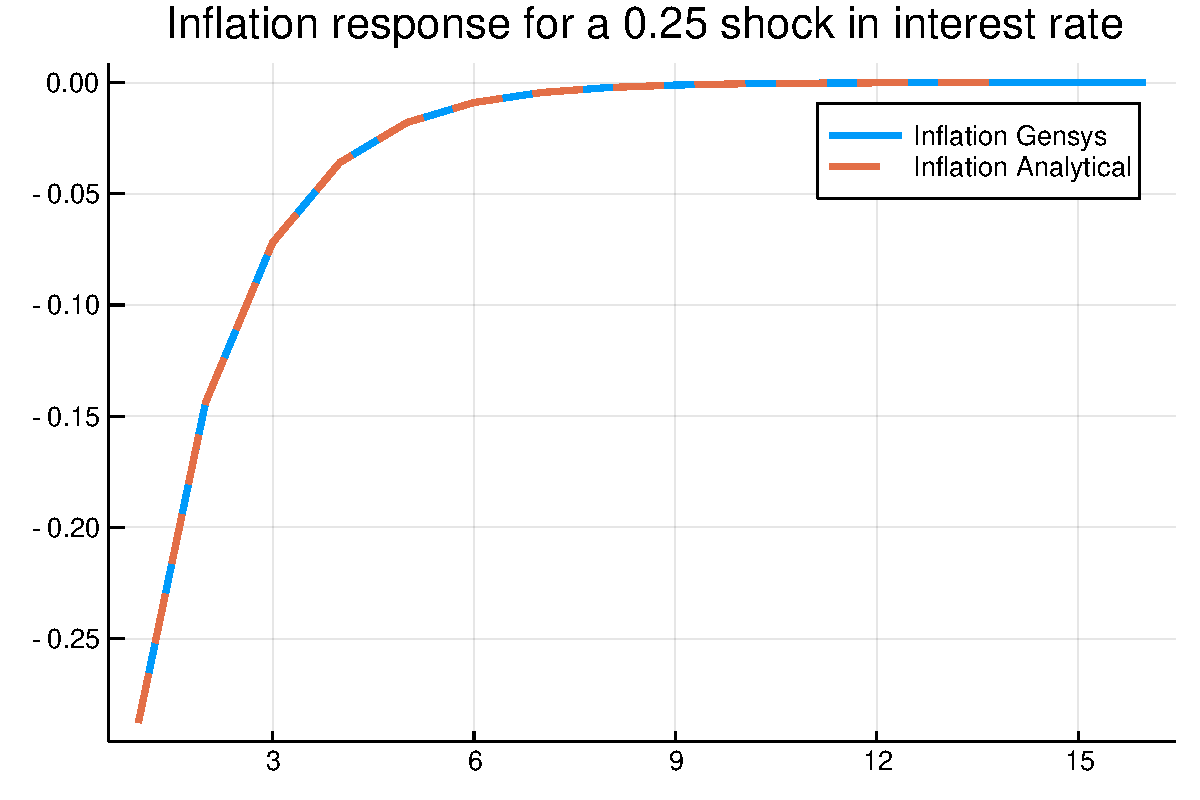
\includegraphics[width=\linewidth]{figures/dsge_and_julia_11_1.pdf}

\begin{lstlisting}
(*@\HLJLnf{plot}@*)(*@\HLJLp{(}@*)(*@\HLJLn{irfs}@*)(*@\HLJLp{[}@*)(*@\HLJLoB{:}@*)(*@\HLJLp{,}@*)(*@\HLJLni{2}@*)(*@\HLJLp{],}@*) (*@\HLJLn{label}@*) (*@\HLJLoB{=}@*) (*@\HLJLs{"{}Output}@*) (*@\HLJLs{Gap}@*) (*@\HLJLs{Gensys"{}}@*)(*@\HLJLp{,}@*) (*@\HLJLn{w}@*) (*@\HLJLoB{=}@*) (*@\HLJLni{3}@*)(*@\HLJLp{)}@*)
(*@\HLJLnf{plot!}@*)(*@\HLJLp{(}@*)(*@\HLJLn{irfs{\_}true}@*)(*@\HLJLp{[}@*)(*@\HLJLni{2}@*)(*@\HLJLoB{:}@*)(*@\HLJLni{15}@*)(*@\HLJLp{,}@*)(*@\HLJLni{2}@*)(*@\HLJLp{],}@*) (*@\HLJLn{label}@*) (*@\HLJLoB{=}@*) (*@\HLJLs{"{}Output}@*) (*@\HLJLs{Gap}@*) (*@\HLJLs{Analytical"{}}@*)(*@\HLJLp{,}@*) (*@\HLJLn{line}@*) (*@\HLJLoB{=}@*) (*@\HLJLsc{:dash}@*)(*@\HLJLp{,}@*) (*@\HLJLn{w}@*) (*@\HLJLoB{=}@*) (*@\HLJLni{3}@*)(*@\HLJLp{)}@*)
(*@\HLJLnf{title!}@*)(*@\HLJLp{(}@*)(*@\HLJLs{"{}Output}@*) (*@\HLJLs{Gap}@*) (*@\HLJLs{response}@*) (*@\HLJLs{for}@*) (*@\HLJLs{a}@*) (*@\HLJLs{0.25}@*) (*@\HLJLs{shock}@*) (*@\HLJLs{in}@*) (*@\HLJLs{interest}@*) (*@\HLJLs{rate"{}}@*)(*@\HLJLp{)}@*)
\end{lstlisting}

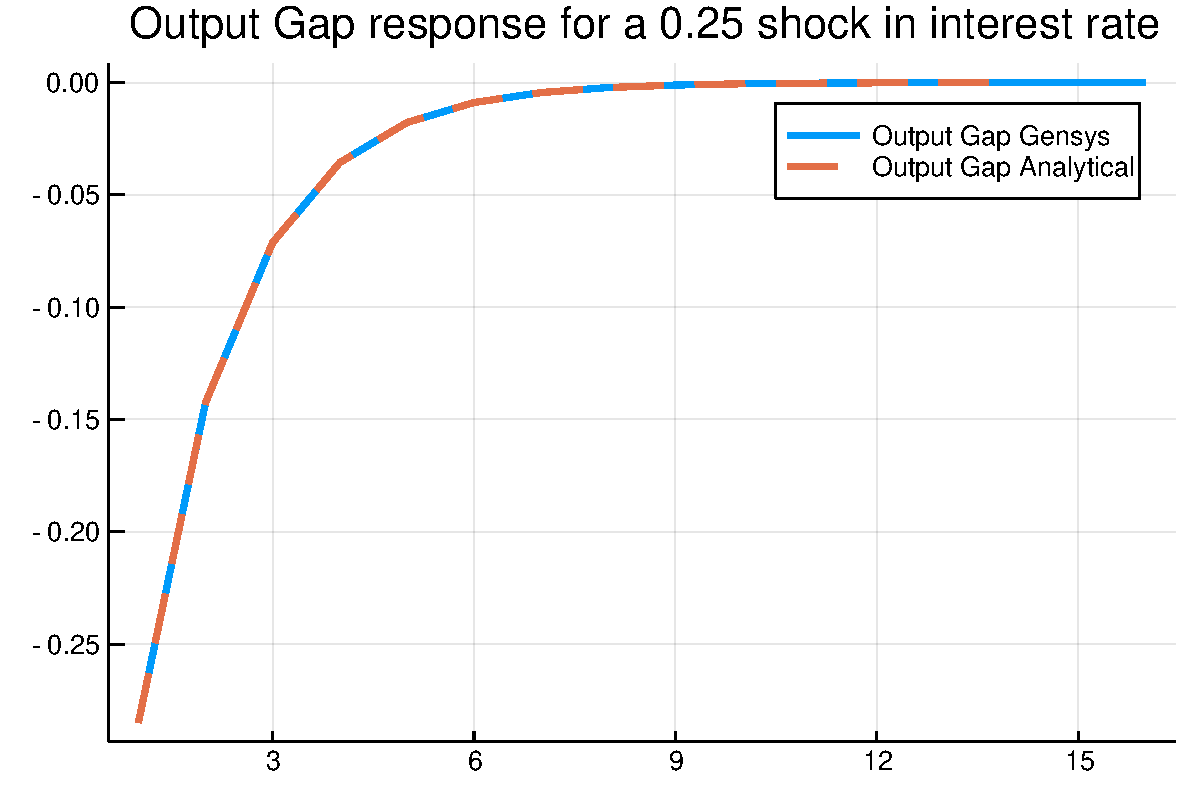
\includegraphics[width=\linewidth]{figures/dsge_and_julia_12_1.pdf}

\begin{lstlisting}
(*@\HLJLnf{plot}@*)(*@\HLJLp{(}@*)(*@\HLJLni{4}@*)(*@\HLJLoB{*}@*)(*@\HLJLn{irfs}@*)(*@\HLJLp{[}@*)(*@\HLJLoB{:}@*)(*@\HLJLp{,}@*)(*@\HLJLni{3}@*)(*@\HLJLp{],}@*) (*@\HLJLn{label}@*) (*@\HLJLoB{=}@*) (*@\HLJLs{"{}Interest}@*) (*@\HLJLs{Rate}@*) (*@\HLJLs{Gensys"{}}@*)(*@\HLJLp{,}@*) (*@\HLJLn{w}@*) (*@\HLJLoB{=}@*) (*@\HLJLni{3}@*)(*@\HLJLp{)}@*)
(*@\HLJLnf{plot!}@*)(*@\HLJLp{(}@*)(*@\HLJLni{4}@*)(*@\HLJLoB{*}@*)(*@\HLJLn{irfs{\_}true}@*)(*@\HLJLp{[}@*)(*@\HLJLni{2}@*)(*@\HLJLoB{:}@*)(*@\HLJLni{15}@*)(*@\HLJLp{,}@*)(*@\HLJLni{3}@*)(*@\HLJLp{],}@*) (*@\HLJLn{label}@*) (*@\HLJLoB{=}@*) (*@\HLJLs{"{}Interest}@*) (*@\HLJLs{Rate}@*) (*@\HLJLs{Analytical"{}}@*)(*@\HLJLp{,}@*) (*@\HLJLn{line}@*) (*@\HLJLoB{=}@*) (*@\HLJLsc{:dash}@*)(*@\HLJLp{,}@*) (*@\HLJLn{w}@*) (*@\HLJLoB{=}@*) (*@\HLJLni{3}@*)(*@\HLJLp{)}@*)
(*@\HLJLnf{title!}@*)(*@\HLJLp{(}@*)(*@\HLJLs{"{}Nominal}@*) (*@\HLJLs{Interest}@*) (*@\HLJLs{response}@*) (*@\HLJLs{for}@*) (*@\HLJLs{a}@*) (*@\HLJLs{0.25}@*) (*@\HLJLs{shock}@*) (*@\HLJLs{in}@*) (*@\HLJLs{interest}@*) (*@\HLJLs{rate"{}}@*)(*@\HLJLp{)}@*)
\end{lstlisting}

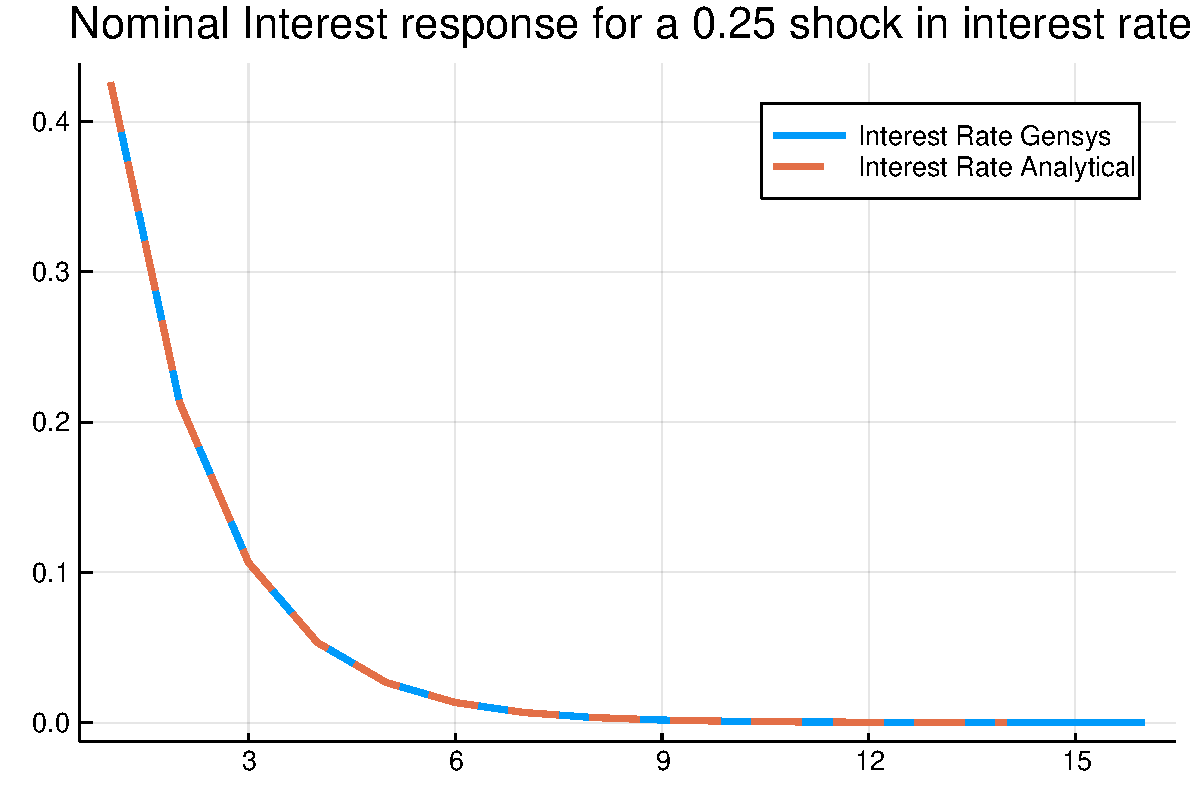
\includegraphics[width=\linewidth]{figures/dsge_and_julia_13_1.pdf}

\begin{lstlisting}
(*@\HLJLnf{plot}@*)(*@\HLJLp{(}@*)(*@\HLJLn{irfs}@*)(*@\HLJLp{[}@*)(*@\HLJLoB{:}@*)(*@\HLJLp{,}@*)(*@\HLJLni{4}@*)(*@\HLJLp{],}@*) (*@\HLJLn{label}@*) (*@\HLJLoB{=}@*) (*@\HLJLs{"{}v}@*) (*@\HLJLs{Gensys"{}}@*)(*@\HLJLp{,}@*) (*@\HLJLn{w}@*) (*@\HLJLoB{=}@*) (*@\HLJLni{3}@*)(*@\HLJLp{)}@*)
(*@\HLJLnf{plot!}@*)(*@\HLJLp{(}@*)(*@\HLJLn{irfs{\_}true}@*)(*@\HLJLp{[}@*)(*@\HLJLni{2}@*)(*@\HLJLoB{:}@*)(*@\HLJLni{15}@*)(*@\HLJLp{,}@*)(*@\HLJLni{4}@*)(*@\HLJLp{],}@*) (*@\HLJLn{label}@*) (*@\HLJLoB{=}@*) (*@\HLJLs{"{}v}@*) (*@\HLJLs{Analytical"{}}@*)(*@\HLJLp{,}@*) (*@\HLJLn{line}@*) (*@\HLJLoB{=}@*) (*@\HLJLsc{:dash}@*)(*@\HLJLp{,}@*) (*@\HLJLn{w}@*) (*@\HLJLoB{=}@*) (*@\HLJLni{3}@*)(*@\HLJLp{)}@*)
(*@\HLJLnf{title!}@*)(*@\HLJLp{(}@*)(*@\HLJLs{"{}v}@*) (*@\HLJLs{response}@*) (*@\HLJLs{for}@*) (*@\HLJLs{a}@*) (*@\HLJLs{0.25}@*) (*@\HLJLs{shock}@*) (*@\HLJLs{in}@*) (*@\HLJLs{interest}@*) (*@\HLJLs{rate"{}}@*)(*@\HLJLp{)}@*)
\end{lstlisting}

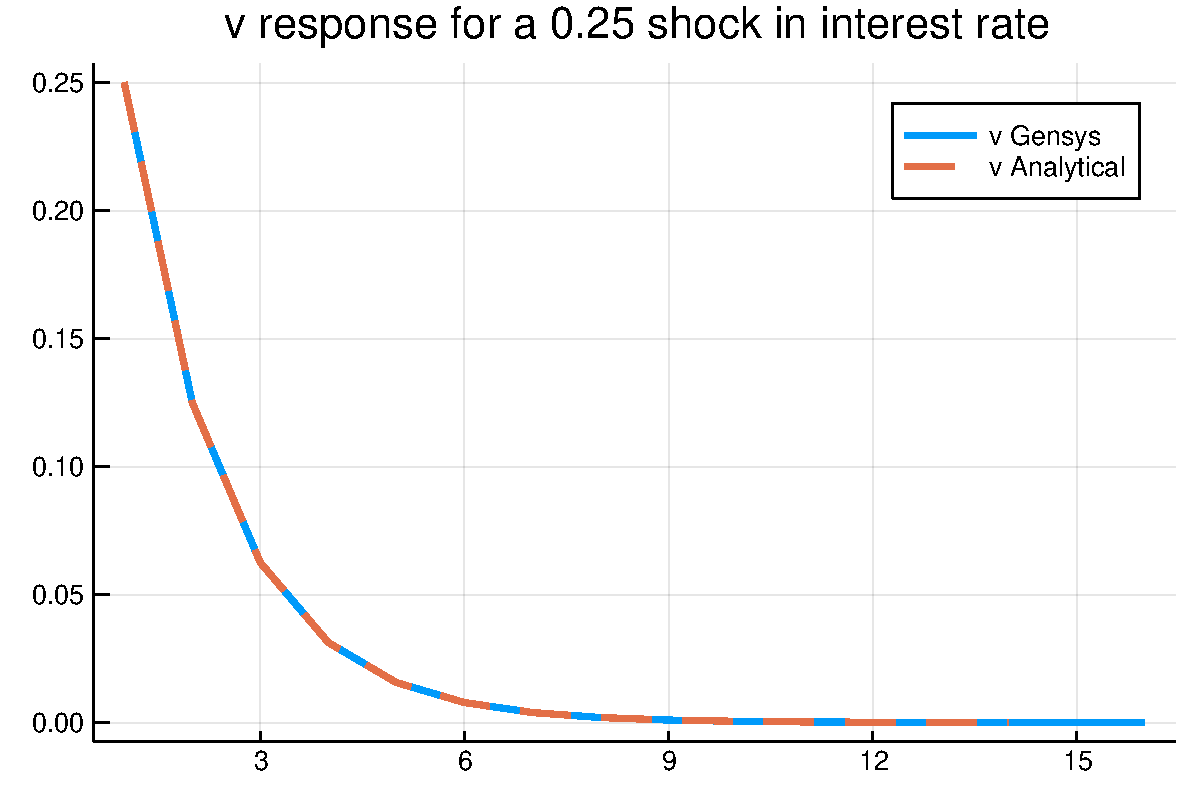
\includegraphics[width=\linewidth]{figures/dsge_and_julia_14_1.pdf}

The impulse response are identical between the two methods, which is a strong evidence of the reliability and precision of our implementation of Gensys, Gensys itself and Julia capabilities to handle linear algebra routines.

\subsection{Likelihood}
The likelihood function is the next step of our code. The inputs are a set of parameter values and data regarding the economy. For a set of parameters, we use gensys to find the VAR representation of the model. We could estimate it as an usual VAR, however:

\begin{enumerate}
	
\item In general, the model assumes that the shock is an autocorrelated process. This means that the true process is a VARMA model and the coefficient of the autocorrelation and the fundamental shocks must be estimated as well.

\item For estimation, one can only include as many data series as there are shocks in the model. Otherwise, we incur in a stochastic singularity, i.e. the whole model is determined for any set of parameters. In this extremely simple example, this forces us to work with a single series. Since the dynamic of the model depends on the evolution of all the series, we have to estimate the remaining series from the data.

\end{enumerate}

The fact that the model is linear with Gaussian shocks allows us to work with the Kalman Filter, that addresses both points above. The Kalman Filter works from the state space representation of the model:

\begin{align} 
y_t = Gx_t + v_t\\
x_t = Ax_{t-1} + w_t
\end{align} 

In which $v_t ~ N(0,R)$ and $w_t ~ N(0,Q)$. The first equation is the \emph{observation equation} and the second one is the \emph{state equation}. The idea is that we observe $y_t$ and that the behaviour of the system is governed by $x_t$ - an idea closely related to the factor model in economics. This assumes asd well that we know $G$,$A$,$R$ and $Q$. This allows us to recover $x_t$ in a recursive manner.

What we do is to set $A$ equals to $\Theta_1$ and $Q$ equals to $\sigma^2 \Theta_2 \Theta_2'$, in which $\Theta_1$ and $\Theta_2$ are the matrices from gensys and $\sigma^2$ is the variance from the monetary policy shock. So our state space is the whole system. $G$ is just a selection matrix, i.e. which of the series from the state space we observe - this is filled with a value of 1 and everything else is just 0.

The value of $R$ is \emph{not} set to zero. The usual interpretation of the shock $v_t$ is that it is a measurement error, i.e. we do not observe the exactly true GDP that our model prescribes because it has measurement errors. However, in our setup there are no such things: we simulate the values from the system and observe them exactly. So, we should set it to zero.

However, it is well known (see, for example, \cite{Keesman2011}) that if there are no measurement errors the Kalman filter suffers from serious numerical instability problems. One that we found is that it often happens that the forecast variance matrix will have a determinant close to zero or even negative if there are no measurement errors. To avoid this, we add a measurement error with variance $10^{-8}$. This creates a really small error and avoids the numerical instability problems completely. We could push it even closer to zero, however due to the finite precision of floating point arithmetic we do not do it. There are ways of avoiding this - \cite{Keesman2011} suggests a root Kalman filter that is more stable from the numerical point of view.

Although this trick helps preventing errors, it does not solve all the problems. Another problem - that is related to taking the inverse of the forecast error variance - is that the matrix might be \emph{ill-condition}. This is related to the condition number of a matrix, $||A|| ||A^{-1}||$. Large condition numbers means that the inverse is an ill posed problem, from the numerical point of view; condition numbers close to one means that the problem is well behaved. We follow Dynare's code in skipping the cases in which the forecast variance matrix is ill conditioned (they use the inverse of the condition number, so numbers closer to zero means that the problem is ill posed. We use the same threshold they use).

Each step of the Kalman filter uses the current distribution about the state to forecast the state in the future. The error from the difference of the forecasted state to the real value of the state gives the mean of the normal. The forecast error variance is $P = G\Sigma_sG' + R$, in which $\Sigma_s$ is the variance matrix of the states. This gives us all we need to evaluate the likelihood at each observation. With the likelihood at each point, one can then \emph{multiply} all of the values.

This is problematic because, in many cases, the value of the density at the point is smaller than 1. Since the computer has a finite decimal precision (known as the \emph{eps}), multiplying several numbers bellow one can quickly become messy. Just as an example, taking $0.0001^{100}$ (this would be just a hundred observations with density 0.0001) is bellow the eps of most CPUs. To avoid this, is better to work with the log of the likelihood and sum them over. That is the procedure we follow.

We also throw away the first nine likelihoods from the state. One needs to initialize the state distribution at some value - since we are working with the Normal distribution, this means the initialize the mean and the variance of the distribution. It takes a while to make this values converge, and in some cases this throws non sense values that destroy the loglikelihood (like $10^{18}$). For initialization, we use the mean and the variance of the observed equation.

Here is the function for the (log)likelihood:


\begin{lstlisting}
(*@\HLJLk{using}@*) (*@\HLJLn{QuantEcon}@*)
(*@\HLJLk{using}@*) (*@\HLJLn{Statistics}@*)
(*@\HLJLk{using}@*) (*@\HLJLn{LinearAlgebra}@*)

(*@\HLJLnf{include}@*)(*@\HLJLp{(}@*)(*@\HLJLnf{string}@*)(*@\HLJLp{(}@*)(*@\HLJLnf{pwd}@*)(*@\HLJLp{(),}@*)(*@\HLJLs{"{}/src/gensys.jl"{}}@*)(*@\HLJLp{))}@*)

(*@\HLJLk{function}@*) (*@\HLJLnf{log{\_}like{\_}dsge}@*)(*@\HLJLp{(}@*)(*@\HLJLn{par}@*)(*@\HLJLp{,}@*)(*@\HLJLn{data}@*)(*@\HLJLp{;}@*)(*@\HLJLn{kalman{\_}tol}@*) (*@\HLJLoB{=}@*) (*@\HLJLnfB{1e-10}@*)(*@\HLJLp{)}@*)
    (*@\HLJLcs{{\#}order}@*) (*@\HLJLcs{to}@*) (*@\HLJLcs{par}@*)
    (*@\HLJLcs{{\#}alfa}@*)
    (*@\HLJLcs{{\#}beta}@*)
    (*@\HLJLcs{{\#}epsilon}@*)
    (*@\HLJLcs{{\#}theta}@*)
    (*@\HLJLcs{{\#}sig}@*)
    (*@\HLJLcs{{\#}sigma:}@*) (*@\HLJLcs{this}@*) (*@\HLJLcs{is}@*) (*@\HLJLcs{the}@*) (*@\HLJLcs{std}@*) (*@\HLJLcs{dev}@*) (*@\HLJLcs{of}@*) (*@\HLJLcs{the}@*) (*@\HLJLcs{innovation}@*)
    (*@\HLJLcs{{\#}phi}@*)
    (*@\HLJLcs{{\#}phi{\_}pi}@*)
    (*@\HLJLcs{{\#}phi{\_}y}@*)
    (*@\HLJLcs{{\#}rho{\_}v}@*)

    (*@\HLJLcs{{\#}data}@*) (*@\HLJLcs{will}@*) (*@\HLJLcs{have}@*) (*@\HLJLcs{t}@*) (*@\HLJLcs{x}@*) (*@\HLJLcs{p}@*) (*@\HLJLcs{dimension:}@*) (*@\HLJLcs{lines}@*) (*@\HLJLcs{are}@*) (*@\HLJLcs{periods}@*) (*@\HLJLcs{p}@*) (*@\HLJLcs{are}@*) (*@\HLJLcs{variables}@*)

    (*@\HLJLn{alfa}@*) (*@\HLJLoB{=}@*) (*@\HLJLn{par}@*)(*@\HLJLp{[}@*)(*@\HLJLni{1}@*)(*@\HLJLp{]}@*)
    (*@\HLJLn{bet}@*) (*@\HLJLoB{=}@*) (*@\HLJLn{par}@*)(*@\HLJLp{[}@*)(*@\HLJLni{2}@*)(*@\HLJLp{]}@*)
    (*@\HLJLn{epsilon}@*) (*@\HLJLoB{=}@*) (*@\HLJLn{par}@*)(*@\HLJLp{[}@*)(*@\HLJLni{3}@*)(*@\HLJLp{]}@*)
    (*@\HLJLn{theta}@*) (*@\HLJLoB{=}@*) (*@\HLJLn{par}@*)(*@\HLJLp{[}@*)(*@\HLJLni{4}@*)(*@\HLJLp{]}@*)
    (*@\HLJLn{sig}@*) (*@\HLJLoB{=}@*) (*@\HLJLn{par}@*)(*@\HLJLp{[}@*)(*@\HLJLni{5}@*)(*@\HLJLp{]}@*)
    (*@\HLJLcs{{\#}par}@*) (*@\HLJLcs{6}@*) (*@\HLJLcs{is}@*) (*@\HLJLcs{coded}@*) (*@\HLJLcs{bellow}@*) (*@\HLJLcs{see}@*) (*@\HLJLcs{line}@*) (*@\HLJLcs{56}@*)
    (*@\HLJLn{phi}@*) (*@\HLJLoB{=}@*) (*@\HLJLn{par}@*)(*@\HLJLp{[}@*)(*@\HLJLni{7}@*)(*@\HLJLp{]}@*)
    (*@\HLJLn{phi{\_}pi}@*) (*@\HLJLoB{=}@*) (*@\HLJLn{par}@*)(*@\HLJLp{[}@*)(*@\HLJLni{8}@*)(*@\HLJLp{]}@*)
    (*@\HLJLn{phi{\_}y}@*) (*@\HLJLoB{=}@*) (*@\HLJLn{par}@*)(*@\HLJLp{[}@*)(*@\HLJLni{9}@*)(*@\HLJLp{]}@*)
    (*@\HLJLn{rho{\_}v}@*) (*@\HLJLoB{=}@*) (*@\HLJLn{par}@*)(*@\HLJLp{[}@*)(*@\HLJLni{10}@*)(*@\HLJLp{]}@*)

    (*@\HLJLn{THETA}@*) (*@\HLJLoB{=}@*) (*@\HLJLp{(}@*)(*@\HLJLni{1}@*)(*@\HLJLoB{-}@*)(*@\HLJLn{alfa}@*)(*@\HLJLp{)}@*)(*@\HLJLoB{/}@*)(*@\HLJLp{(}@*)(*@\HLJLni{1}@*)(*@\HLJLoB{-}@*)(*@\HLJLn{alfa}@*)(*@\HLJLoB{+}@*)(*@\HLJLn{alfa}@*)(*@\HLJLoB{*}@*)(*@\HLJLn{epsilon}@*)(*@\HLJLp{)}@*)
    (*@\HLJLn{lamb}@*) (*@\HLJLoB{=}@*) (*@\HLJLp{(}@*)(*@\HLJLni{1}@*)(*@\HLJLoB{-}@*)(*@\HLJLn{theta}@*)(*@\HLJLp{)}@*)(*@\HLJLoB{*}@*)(*@\HLJLp{(}@*)(*@\HLJLni{1}@*)(*@\HLJLoB{-}@*)(*@\HLJLn{bet}@*)(*@\HLJLoB{*}@*)(*@\HLJLn{theta}@*)(*@\HLJLp{)}@*)(*@\HLJLoB{/}@*)(*@\HLJLn{theta}@*)(*@\HLJLoB{*}@*)(*@\HLJLn{THETA}@*)
    (*@\HLJLn{kappa}@*) (*@\HLJLoB{=}@*) (*@\HLJLn{lamb}@*)(*@\HLJLoB{*}@*)(*@\HLJLp{(}@*)(*@\HLJLn{sig}@*)(*@\HLJLoB{+}@*)(*@\HLJLp{(}@*)(*@\HLJLn{phi}@*)(*@\HLJLoB{+}@*)(*@\HLJLn{alfa}@*)(*@\HLJLp{)}@*)(*@\HLJLoB{/}@*)(*@\HLJLp{(}@*)(*@\HLJLni{1}@*)(*@\HLJLoB{-}@*)(*@\HLJLn{alfa}@*)(*@\HLJLp{))}@*)

    (*@\HLJLn{nobs}@*) (*@\HLJLoB{=}@*) (*@\HLJLnf{size}@*)(*@\HLJLp{(}@*)(*@\HLJLn{data}@*)(*@\HLJLp{,}@*)(*@\HLJLni{1}@*)(*@\HLJLp{)}@*)

    (*@\HLJLn{GAMMA{\_}0}@*) (*@\HLJLoB{=}@*) (*@\HLJLp{[}@*)(*@\HLJLn{bet}@*)  (*@\HLJLni{0}@*)    (*@\HLJLni{0}@*)  (*@\HLJLni{0}@*)(*@\HLJLp{;}@*)
               (*@\HLJLni{1}@*)    (*@\HLJLn{sig}@*)  (*@\HLJLni{0}@*)  (*@\HLJLni{0}@*)(*@\HLJLp{;}@*)
               (*@\HLJLni{0}@*)    (*@\HLJLni{0}@*)    (*@\HLJLni{0}@*)  (*@\HLJLni{0}@*)(*@\HLJLp{;}@*)
               (*@\HLJLni{0}@*)    (*@\HLJLni{0}@*)    (*@\HLJLni{0}@*)  (*@\HLJLni{1}@*)(*@\HLJLp{]}@*)

    (*@\HLJLn{GAMMA{\_}1}@*) (*@\HLJLoB{=}@*) (*@\HLJLp{[}@*) (*@\HLJLni{1}@*)       (*@\HLJLoB{-}@*)(*@\HLJLn{kappa}@*)  (*@\HLJLni{0}@*)   (*@\HLJLni{0}@*)(*@\HLJLp{;}@*)
                (*@\HLJLni{0}@*)        (*@\HLJLn{sig}@*)    (*@\HLJLni{1}@*)   (*@\HLJLni{0}@*)(*@\HLJLp{;}@*)
               (*@\HLJLoB{-}@*)(*@\HLJLn{phi{\_}pi}@*)  (*@\HLJLoB{-}@*)(*@\HLJLn{phi{\_}y}@*)  (*@\HLJLni{1}@*)  (*@\HLJLoB{-}@*)(*@\HLJLni{1}@*)(*@\HLJLp{;}@*)
                (*@\HLJLni{0}@*)        (*@\HLJLni{0}@*)      (*@\HLJLni{0}@*)   (*@\HLJLn{rho{\_}v}@*)(*@\HLJLp{]}@*)

    (*@\HLJLn{PSI}@*) (*@\HLJLoB{=}@*) (*@\HLJLp{[}@*)(*@\HLJLni{0}@*)(*@\HLJLp{;}@*) (*@\HLJLni{0}@*)(*@\HLJLp{;}@*) (*@\HLJLni{0}@*)(*@\HLJLp{;}@*) (*@\HLJLni{1}@*)(*@\HLJLp{]}@*)

    (*@\HLJLn{PI}@*) (*@\HLJLoB{=}@*) (*@\HLJLp{[}@*)(*@\HLJLn{bet}@*)  (*@\HLJLni{0}@*)(*@\HLJLp{;}@*)
          (*@\HLJLni{1}@*)    (*@\HLJLn{sig}@*)(*@\HLJLp{;}@*)
          (*@\HLJLni{0}@*)    (*@\HLJLni{0}@*)(*@\HLJLp{;}@*)
          (*@\HLJLni{0}@*)    (*@\HLJLni{0}@*)(*@\HLJLp{]}@*)

    (*@\HLJLn{p}@*) (*@\HLJLoB{=}@*) (*@\HLJLnf{size}@*)(*@\HLJLp{(}@*)(*@\HLJLn{GAMMA{\_}1}@*)(*@\HLJLp{,}@*)(*@\HLJLni{1}@*)(*@\HLJLp{)}@*) (*@\HLJLcs{{\#}number}@*) (*@\HLJLcs{of}@*) (*@\HLJLcs{endogenous}@*) (*@\HLJLcs{vars}@*)

    (*@\HLJLn{sol}@*) (*@\HLJLoB{=}@*) (*@\HLJLnf{gensys}@*)(*@\HLJLp{(}@*)(*@\HLJLn{GAMMA{\_}0}@*)(*@\HLJLp{,}@*)(*@\HLJLn{GAMMA{\_}1}@*)(*@\HLJLp{,}@*)(*@\HLJLn{PSI}@*)(*@\HLJLp{,}@*)(*@\HLJLn{PI}@*)(*@\HLJLp{;}@*) (*@\HLJLn{verbose}@*) (*@\HLJLoB{=}@*) (*@\HLJLkc{false}@*)(*@\HLJLp{)}@*)
    (*@\HLJLk{if}@*) (*@\HLJLnf{sum}@*)(*@\HLJLp{(}@*)(*@\HLJLn{sol}@*)(*@\HLJLoB{.}@*)(*@\HLJLn{eu}@*)(*@\HLJLp{)}@*) (*@\HLJLoB{!=}@*) (*@\HLJLni{2}@*)
        (*@\HLJLk{return}@*) (*@\HLJLoB{-}@*)(*@\HLJLn{NaN}@*)
    (*@\HLJLk{end}@*)

    (*@\HLJLcs{{\#}Sig}@*) (*@\HLJLcs{=}@*) (*@\HLJLcs{zeros(p,p)}@*)
    (*@\HLJLcs{{\#}Sig[4,4]}@*) (*@\HLJLcs{=}@*) (*@\HLJLcs{par[6]}@*)

    (*@\HLJLn{G}@*) (*@\HLJLoB{=}@*) (*@\HLJLnf{zeros}@*)(*@\HLJLp{(}@*)(*@\HLJLni{1}@*)(*@\HLJLp{,}@*)(*@\HLJLn{p}@*)(*@\HLJLp{)}@*)
    (*@\HLJLn{G}@*)(*@\HLJLp{[}@*)(*@\HLJLni{1}@*)(*@\HLJLp{,}@*)(*@\HLJLni{2}@*)(*@\HLJLp{]}@*) (*@\HLJLoB{=}@*) (*@\HLJLni{1}@*)

    (*@\HLJLn{A}@*) (*@\HLJLoB{=}@*) (*@\HLJLn{sol}@*)(*@\HLJLoB{.}@*)(*@\HLJLn{Theta1}@*)
    (*@\HLJLn{R}@*) (*@\HLJLoB{=}@*) (*@\HLJLp{[}@*)(*@\HLJLni{0}@*)(*@\HLJLp{]}@*) (*@\HLJLoB{.+}@*) (*@\HLJLnfB{1e-8}@*)
    (*@\HLJLn{Q}@*) (*@\HLJLoB{=}@*) (*@\HLJLn{par}@*)(*@\HLJLp{[}@*)(*@\HLJLni{6}@*)(*@\HLJLp{]}@*)(*@\HLJLoB{{\textasciicircum}}@*)(*@\HLJLni{2}@*)(*@\HLJLoB{*}@*)(*@\HLJLn{sol}@*)(*@\HLJLoB{.}@*)(*@\HLJLn{Theta2}@*)(*@\HLJLoB{*}@*)(*@\HLJLn{sol}@*)(*@\HLJLoB{.}@*)(*@\HLJLn{Theta2}@*)(*@\HLJLoB{{\textquotesingle}}@*)

    (*@\HLJLn{kalman{\_}res}@*) (*@\HLJLoB{=}@*) (*@\HLJLnf{Kalman}@*)(*@\HLJLp{(}@*)(*@\HLJLn{A}@*)(*@\HLJLp{,}@*)(*@\HLJLn{G}@*)(*@\HLJLp{,}@*)(*@\HLJLn{Q}@*)(*@\HLJLp{,}@*)(*@\HLJLn{R}@*)(*@\HLJLp{)}@*) (*@\HLJLcs{{\#}create}@*) (*@\HLJLcs{a}@*) (*@\HLJLcs{Kalman}@*) (*@\HLJLcs{filter}@*) (*@\HLJLcs{instance}@*)

    (*@\HLJLn{y{\_}mean}@*) (*@\HLJLoB{=}@*) (*@\HLJLnf{mean}@*)(*@\HLJLp{(}@*)(*@\HLJLn{data}@*)(*@\HLJLp{,}@*)(*@\HLJLn{dims}@*)(*@\HLJLoB{=}@*)(*@\HLJLni{1}@*)(*@\HLJLp{)}@*)
    (*@\HLJLn{y{\_}var}@*) (*@\HLJLoB{=}@*) (*@\HLJLnf{var}@*)(*@\HLJLp{(}@*)(*@\HLJLn{data}@*)(*@\HLJLp{,}@*)(*@\HLJLn{dims}@*)(*@\HLJLoB{=}@*)(*@\HLJLni{1}@*)(*@\HLJLp{)}@*)
    (*@\HLJLn{y{\_}var}@*) (*@\HLJLoB{=}@*) (*@\HLJLnf{reshape}@*)(*@\HLJLp{(}@*)(*@\HLJLn{y{\_}var}@*)(*@\HLJLp{,}@*)(*@\HLJLnf{size}@*)(*@\HLJLp{(}@*)(*@\HLJLn{y{\_}var}@*)(*@\HLJLp{,}@*)(*@\HLJLni{2}@*)(*@\HLJLp{))}@*)
    (*@\HLJLcs{{\#}y{\_}var}@*) (*@\HLJLcs{=}@*) (*@\HLJLcs{repeat([1],p)}@*)

    (*@\HLJLn{x{\_}hat}@*) (*@\HLJLoB{=}@*) (*@\HLJLnf{repeat}@*)(*@\HLJLp{(}@*)(*@\HLJLn{y{\_}mean}@*)(*@\HLJLp{,}@*)(*@\HLJLn{p}@*)(*@\HLJLp{)}@*) (*@\HLJLcs{{\#}initial}@*) (*@\HLJLcs{mean}@*) (*@\HLJLcs{of}@*) (*@\HLJLcs{the}@*) (*@\HLJLcs{state}@*)
    (*@\HLJLn{x{\_}var}@*) (*@\HLJLoB{=}@*) (*@\HLJLnf{diagm}@*)(*@\HLJLp{(}@*)(*@\HLJLnf{repeat}@*)(*@\HLJLp{(}@*)(*@\HLJLn{y{\_}var}@*)(*@\HLJLp{,}@*)(*@\HLJLn{p}@*)(*@\HLJLp{))}@*)(*@\HLJLcs{{\#}variance}@*) (*@\HLJLcs{initial}@*) (*@\HLJLcs{of}@*) (*@\HLJLcs{state}@*)
    (*@\HLJLcs{{\#}x{\_}var}@*) (*@\HLJLcs{=}@*) (*@\HLJLcs{x{\_}var*x{\_}var{\textquotesingle}}@*)
    (*@\HLJLnf{set{\_}state!}@*)(*@\HLJLp{(}@*)(*@\HLJLn{kalman{\_}res}@*)(*@\HLJLp{,}@*)(*@\HLJLn{x{\_}hat}@*)(*@\HLJLp{,}@*)(*@\HLJLn{x{\_}var}@*)(*@\HLJLp{)}@*)

    (*@\HLJLn{fit}@*) (*@\HLJLoB{=}@*) (*@\HLJLnf{zeros}@*)(*@\HLJLp{(}@*)(*@\HLJLn{nobs}@*)(*@\HLJLp{,}@*)(*@\HLJLni{4}@*)(*@\HLJLp{)}@*)

    (*@\HLJLn{llh}@*) (*@\HLJLoB{=}@*) (*@\HLJLnf{zeros}@*)(*@\HLJLp{(}@*)(*@\HLJLn{nobs}@*)(*@\HLJLp{)}@*)

    (*@\HLJLk{for}@*) (*@\HLJLn{j}@*) (*@\HLJLkp{in}@*) (*@\HLJLni{1}@*)(*@\HLJLoB{:}@*)(*@\HLJLp{(}@*)(*@\HLJLn{nobs}@*)(*@\HLJLoB{-}@*)(*@\HLJLni{1}@*)(*@\HLJLp{)}@*)
        (*@\HLJLn{med}@*) (*@\HLJLoB{=}@*) (*@\HLJLn{kalman{\_}res}@*)(*@\HLJLoB{.}@*)(*@\HLJLn{cur{\_}x{\_}hat}@*)
        (*@\HLJLn{fit}@*)(*@\HLJLp{[}@*)(*@\HLJLn{j}@*)(*@\HLJLp{,}@*)(*@\HLJLoB{:}@*)(*@\HLJLp{]}@*) (*@\HLJLoB{=}@*) (*@\HLJLn{med}@*)
        (*@\HLJLn{varian}@*) (*@\HLJLoB{=}@*) (*@\HLJLn{kalman{\_}res}@*)(*@\HLJLoB{.}@*)(*@\HLJLn{cur{\_}sigma}@*)
        (*@\HLJLcs{{\#}println(det(varian))}@*)
        (*@\HLJLn{eta}@*) (*@\HLJLoB{=}@*) (*@\HLJLn{data}@*)(*@\HLJLp{[}@*)(*@\HLJLn{j}@*)(*@\HLJLoB{+}@*)(*@\HLJLni{1}@*)(*@\HLJLp{,}@*)(*@\HLJLoB{:}@*)(*@\HLJLp{]}@*) (*@\HLJLoB{-}@*) (*@\HLJLn{kalman{\_}res}@*)(*@\HLJLoB{.}@*)(*@\HLJLn{G}@*)(*@\HLJLoB{*}@*)(*@\HLJLn{med}@*) (*@\HLJLcs{{\#}mean}@*) (*@\HLJLcs{loglike}@*)
        (*@\HLJLn{P}@*) (*@\HLJLoB{=}@*) (*@\HLJLn{kalman{\_}res}@*)(*@\HLJLoB{.}@*)(*@\HLJLn{G}@*)(*@\HLJLoB{*}@*)(*@\HLJLn{varian}@*)(*@\HLJLoB{*}@*)(*@\HLJLn{kalman{\_}res}@*)(*@\HLJLoB{.}@*)(*@\HLJLn{G}@*)(*@\HLJLoB{{\textquotesingle}}@*) (*@\HLJLoB{+}@*) (*@\HLJLn{kalman{\_}res}@*)(*@\HLJLoB{.}@*)(*@\HLJLn{R}@*)
        (*@\HLJLn{teste{\_}cond}@*) (*@\HLJLoB{=}@*) (*@\HLJLni{1}@*)(*@\HLJLoB{/}@*)(*@\HLJLnf{cond}@*)(*@\HLJLp{(}@*)(*@\HLJLn{P}@*)(*@\HLJLp{)}@*)
        (*@\HLJLk{if}@*) (*@\HLJLn{teste{\_}cond}@*) (*@\HLJLoB{<}@*) (*@\HLJLn{kalman{\_}tol}@*)
            (*@\HLJLn{llh}@*)(*@\HLJLp{[}@*)(*@\HLJLn{j}@*)(*@\HLJLp{]}@*) (*@\HLJLoB{=}@*) (*@\HLJLoB{-}@*)(*@\HLJLni{500}@*)
        (*@\HLJLcs{{\#}elseif}@*) (*@\HLJLcs{det(P)}@*) (*@\HLJLcs{<=}@*) (*@\HLJLcs{0}@*)
        (*@\HLJLcs{{\#}}@*)    (*@\HLJLcs{llh[j]}@*) (*@\HLJLcs{=}@*) (*@\HLJLcs{-500}@*)
        (*@\HLJLk{else}@*)
            (*@\HLJLn{llh}@*)(*@\HLJLp{[}@*)(*@\HLJLn{j}@*)(*@\HLJLp{]}@*) (*@\HLJLoB{=}@*) (*@\HLJLoB{-}@*)(*@\HLJLp{(}@*)(*@\HLJLn{p}@*)(*@\HLJLoB{*}@*)(*@\HLJLnf{log}@*)(*@\HLJLp{(}@*)(*@\HLJLni{2}@*)(*@\HLJLoB{*}@*)(*@\HLJLn{pi}@*)(*@\HLJLp{)}@*) (*@\HLJLoB{+}@*) (*@\HLJLnf{logdet}@*)(*@\HLJLp{(}@*)(*@\HLJLn{P}@*)(*@\HLJLp{)}@*) (*@\HLJLoB{.+}@*) (*@\HLJLn{eta}@*)(*@\HLJLoB{{\textquotesingle}*}@*)(*@\HLJLnf{inv}@*)(*@\HLJLp{(}@*)(*@\HLJLn{P}@*)(*@\HLJLp{)}@*)(*@\HLJLoB{*}@*)(*@\HLJLn{eta}@*)(*@\HLJLp{)}@*)(*@\HLJLoB{/}@*)(*@\HLJLni{2}@*)
            (*@\HLJLn{QuantEcon}@*)(*@\HLJLoB{.}@*)(*@\HLJLnf{update!}@*)(*@\HLJLp{(}@*)(*@\HLJLn{kalman{\_}res}@*)(*@\HLJLp{,}@*)(*@\HLJLn{data}@*)(*@\HLJLp{[}@*)(*@\HLJLn{j}@*)(*@\HLJLoB{+}@*)(*@\HLJLni{1}@*)(*@\HLJLp{,}@*)(*@\HLJLoB{:}@*)(*@\HLJLp{])}@*) (*@\HLJLcs{{\#}updating}@*) (*@\HLJLcs{the}@*) (*@\HLJLcs{kalman}@*) (*@\HLJLcs{estimates}@*)
        (*@\HLJLk{end}@*)
        (*@\HLJLcs{{\#}println(kalman{\_}res.cur{\_}sigma)}@*)
        (*@\HLJLcs{{\#}println(det(varian))}@*)
        (*@\HLJLcs{{\#}println(P)}@*)
    (*@\HLJLk{end}@*)
    (*@\HLJLn{llh}@*) (*@\HLJLoB{=}@*) (*@\HLJLn{llh}@*)(*@\HLJLp{[}@*)(*@\HLJLni{10}@*)(*@\HLJLoB{:}@*)(*@\HLJLnf{length}@*)(*@\HLJLp{(}@*)(*@\HLJLn{llh}@*)(*@\HLJLp{)]}@*)
    (*@\HLJLk{return}@*) (*@\HLJLnf{sum}@*)(*@\HLJLp{(}@*)(*@\HLJLn{llh}@*)(*@\HLJLp{)}@*)
(*@\HLJLk{end}@*)
\end{lstlisting}


\subsubsection{Example}

Lets simulate an economy using the parameters from Galí's book:


\begin{lstlisting}
(*@\HLJLn{Random}@*)(*@\HLJLoB{.}@*)(*@\HLJLnf{seed!}@*)(*@\HLJLp{(}@*)(*@\HLJLni{324128}@*)(*@\HLJLp{)}@*)

(*@\HLJLnf{include}@*)(*@\HLJLp{(}@*)(*@\HLJLnf{string}@*)(*@\HLJLp{(}@*)(*@\HLJLnf{pwd}@*)(*@\HLJLp{(),}@*)(*@\HLJLs{"{}/src/simulation.jl"{}}@*)(*@\HLJLp{))}@*)

(*@\HLJLn{dados}@*)(*@\HLJLp{,}@*)(*@\HLJLn{choques}@*) (*@\HLJLoB{=}@*) (*@\HLJLnf{simulate{\_}dsge}@*)(*@\HLJLp{(}@*)(*@\HLJLn{GAMMA{\_}0}@*)(*@\HLJLp{,}@*)(*@\HLJLn{GAMMA{\_}1}@*)(*@\HLJLp{,}@*)(*@\HLJLn{PSI}@*)(*@\HLJLp{,}@*)(*@\HLJLn{PI}@*)(*@\HLJLp{,}@*)(*@\HLJLni{5000}@*)(*@\HLJLp{)}@*)
\end{lstlisting}


Now compute the likelihood for beta


\begin{lstlisting}
(*@\HLJLn{bett}@*) (*@\HLJLoB{=}@*) (*@\HLJLnfB{0.70}@*)(*@\HLJLoB{:}@*)(*@\HLJLnfB{0.005}@*)(*@\HLJLoB{:}@*)(*@\HLJLnfB{1.15}@*)

(*@\HLJLn{vals{\_}bet}@*) (*@\HLJLoB{=}@*) (*@\HLJLnf{collect}@*)(*@\HLJLp{(}@*)(*@\HLJLn{bett}@*)(*@\HLJLp{)}@*)

(*@\HLJLk{for}@*) (*@\HLJLn{i}@*) (*@\HLJLkp{in}@*) (*@\HLJLni{1}@*)(*@\HLJLoB{:}@*)(*@\HLJLnf{length}@*)(*@\HLJLp{(}@*)(*@\HLJLn{bett}@*)(*@\HLJLp{)}@*)
    (*@\HLJLn{param1}@*) (*@\HLJLoB{=}@*) (*@\HLJLp{[}@*)(*@\HLJLn{alfa}@*)(*@\HLJLp{,}@*)(*@\HLJLn{bett}@*)(*@\HLJLp{[}@*)(*@\HLJLn{i}@*)(*@\HLJLp{],}@*)(*@\HLJLn{epsilon}@*)(*@\HLJLp{,}@*)(*@\HLJLn{theta}@*)(*@\HLJLp{,}@*)(*@\HLJLn{sig}@*)(*@\HLJLp{,}@*)(*@\HLJLni{1}@*)(*@\HLJLp{,}@*)(*@\HLJLn{phi}@*)(*@\HLJLp{,}@*)(*@\HLJLn{phi{\_}pi}@*)(*@\HLJLp{,}@*)(*@\HLJLn{phi{\_}y}@*)(*@\HLJLp{,}@*)(*@\HLJLn{rho{\_}v}@*)(*@\HLJLp{]}@*)
    (*@\HLJLn{vals{\_}bet}@*)(*@\HLJLp{[}@*)(*@\HLJLn{i}@*)(*@\HLJLp{]}@*) (*@\HLJLoB{=}@*) (*@\HLJLnf{log{\_}like{\_}dsge}@*)(*@\HLJLp{(}@*)(*@\HLJLn{param1}@*)(*@\HLJLp{,}@*)(*@\HLJLn{dados}@*)(*@\HLJLp{[}@*)(*@\HLJLoB{:}@*)(*@\HLJLp{,}@*)(*@\HLJLni{2}@*)(*@\HLJLp{])}@*)
(*@\HLJLk{end}@*)

(*@\HLJLnf{plot}@*)(*@\HLJLp{(}@*)(*@\HLJLn{bett}@*)(*@\HLJLp{,}@*)(*@\HLJLn{vals{\_}bet}@*)(*@\HLJLp{,}@*) (*@\HLJLn{label}@*) (*@\HLJLoB{=}@*) (*@\HLJLs{"{}Likelihood"{}}@*)(*@\HLJLp{)}@*)
(*@\HLJLnf{vline!}@*)(*@\HLJLp{([}@*)(*@\HLJLnfB{0.99}@*)(*@\HLJLp{],}@*) (*@\HLJLn{label}@*) (*@\HLJLoB{=}@*) (*@\HLJLs{"{}True}@*) (*@\HLJLs{Value"{}}@*)(*@\HLJLp{)}@*)
\end{lstlisting}

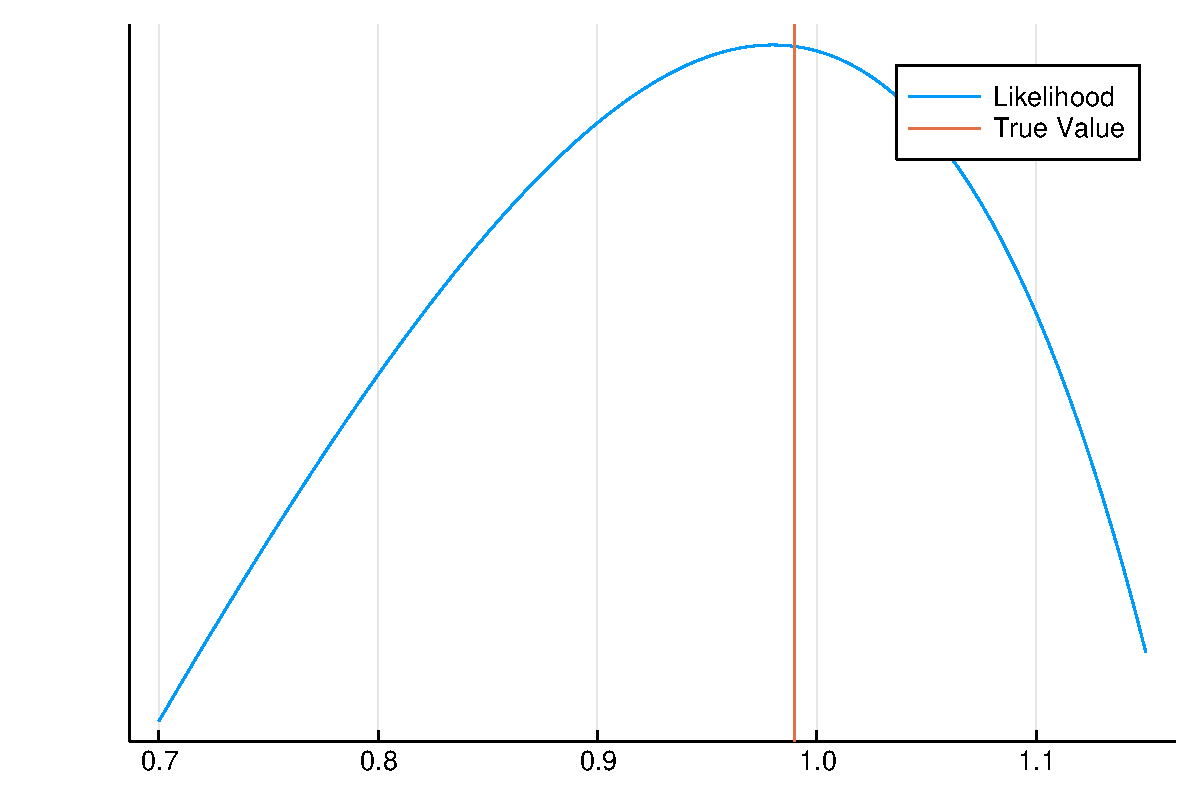
\includegraphics[width=\linewidth]{figures/dsge_and_julia_17_1.pdf}

The shape is what we expected: increasing or decreasing the parameter from some point near the true value should decrease the likelihood. Notice that the maximum of this function is not exactly in the true value of the parameter - even though we have a sample of size 5000, many times the size of the usual macroeconomics database.

\subsection{Markov Chain Monte Carlo}
Bayesian estimation is based around Bayes's Theorem:

\[
P(\Theta|y) = \frac{\ell(y|\Theta)p(\theta)}{P(y)}
\]
In which $\Theta$ is the vector of parameters, $y$ is the data, $\ell$ is the likelihood function, $p(\Theta)$ is the prior over the parameters and $P(y)$ is the marginal over the data. $P(y)$ actually depends of integrals over all the parameters, and so we suffer the curse of dimensionality. Markov Chain Monte Carlo (MCMC) solve this by avoiding estimating $P(y)$ and instead relying on the reason $\frac{\ell(y|\Theta)p(\theta)}{\ell(y|\Theta')p(\theta')}$ to build the posterior. The algorithm is rather simple. Besides the prior and the likelihood, we will also need a kernel distribution, that we will call $\mathcal{K}(\Theta|\Theta')$. Here is the algorithm for a special and rather useful algorithm for MCMC, the Metropolis-Hasting:

For j in 1:ndraws:

\begin{itemize}
\item[1. ] Draw a vector of parameters $\Theta^{*}$, from the distribution $\mathcal{K}(\Theta|\Theta_j)$.


\item[2. ] Compute $r = \min\left\{\frac{\ell(y|\Theta^*)p(\Theta^*)\mathcal{K}(\Theta_{j-1}|\Theta^*)}{\ell(y|\Theta_{j-1})p(\Theta_{j-1})\mathcal{K}(\Theta^*|\Theta_{j-1})},1\right\}$


\item[3. ] Draw a random number from a $\alpha = U(0,1)$


\item[4. ] If $r < \alpha$, set $\Theta_j = \Theta_{j-1}$; otherwise, set $\Theta_j = \Theta^{*}$

\end{itemize}
end

In the end we have $\{\Theta_j\}_{j=1}^{ndraws}$, a set of ndraws of the parameter vector.This algorithm maps the posterior, and is quite smart: every time you draw a parameter vector that makes the likelihood times the prior increase a lot compared to the point you are now, you accept. However, even when it does not increase the likelihood, this does not means that the vector will be excluded: it has some probability of being included. This allows the algorithm to map the distribution and to not get stuck in some points of high probability, like the mode.

The choice of the kernel is important. Usually, the kernel is a Normal distribution that has mean in the last parameter vector accepted (therefore the random walk part of the name that we used in the introduction). The choice of the variance is of central importance: the optimal choice for the variance of the kernel is $c\Sigma_\Theta$, in which $\Sigma_\Theta$ is the variance matrix for the vector $\Theta$ evaluated on the mode. $c$ is a scale constant that plays a fundamental role to ensure that we will map the whole distribution. The idea is simple: if the variance is too low, you will visit only a small part of the distribution in a given number of iterations; set it too high and the algorithm will start to wander in regions far away from the mode, that contribute little to the overall density. Therefore setting $c$ in the right way ensures that our iterations won't be wasted.

Notice that our previous discussion about multiplying small numbers also applies when taking the ratio of two (potentially) small numbers. Therefore, although we could get the likelihood from the log likelihood (just apply the exponential), we do not do it. Instead, step 3 becomes:

\[
r = \min\{0,\log(\ell(y|\Theta^{*})) + \log(p(\Theta^{*})) + \log(\mathcal{K}(\Theta_{j-1}|\Theta^*)) - \log(\ell(y|\Theta_{j-1})) + \log(p(\Theta_{j-1})) + \log(\mathcal{K}(\Theta^{*}|\Theta_{j-1}))\}
\]
And we use $\log(\alpha)$ instead of $\alpha$ in step 4. We tried working with the exponential of the loglikelihood. However, this was not entirely sucessful. On a side note, this trick is not mentioned in any of the books we checked, for example \cite{Canova2011}.

Here are the priors. We create the function \texttt{gamma\_mv} that receives the mean and the standard deviation we want the prior to have, instead of the usual shape and scale parameters:


\begin{lstlisting}
(*@\HLJLk{using}@*) (*@\HLJLn{Distributions}@*)

(*@\HLJLnf{gamma{\_}mv}@*)(*@\HLJLp{(}@*)(*@\HLJLn{mu}@*)(*@\HLJLp{,}@*)(*@\HLJLn{std}@*)(*@\HLJLp{)}@*) (*@\HLJLoB{=}@*) (*@\HLJLnf{Gamma}@*)(*@\HLJLp{(}@*)(*@\HLJLn{mu}@*)(*@\HLJLoB{{\textasciicircum}}@*)(*@\HLJLni{2}@*)(*@\HLJLoB{/}@*)(*@\HLJLn{std}@*)(*@\HLJLoB{{\textasciicircum}}@*)(*@\HLJLni{2}@*)(*@\HLJLp{,}@*)(*@\HLJLn{std}@*)(*@\HLJLoB{{\textasciicircum}}@*)(*@\HLJLni{2}@*)(*@\HLJLoB{/}@*)(*@\HLJLn{mu}@*)(*@\HLJLp{)}@*)
(*@\HLJLnf{gammainv{\_}mv}@*)(*@\HLJLp{(}@*)(*@\HLJLn{mu}@*)(*@\HLJLp{,}@*)(*@\HLJLn{std}@*)(*@\HLJLp{)}@*) (*@\HLJLoB{=}@*) (*@\HLJLnf{Gamma}@*)(*@\HLJLp{(}@*)(*@\HLJLn{mu}@*)(*@\HLJLoB{{\textasciicircum}}@*)(*@\HLJLni{2}@*)(*@\HLJLoB{/}@*)(*@\HLJLn{std}@*)(*@\HLJLoB{{\textasciicircum}}@*)(*@\HLJLni{2}@*)(*@\HLJLp{,(}@*)(*@\HLJLn{std}@*)(*@\HLJLoB{{\textasciicircum}}@*)(*@\HLJLni{2}@*)(*@\HLJLoB{/}@*)(*@\HLJLn{mu}@*)(*@\HLJLp{)}@*)(*@\HLJLoB{{\textasciicircum}}@*)(*@\HLJLp{(}@*)(*@\HLJLoB{-}@*)(*@\HLJLni{1}@*)(*@\HLJLp{))}@*)

(*@\HLJLn{prior{\_}bet}@*) (*@\HLJLoB{=}@*) (*@\HLJLnf{Beta}@*)(*@\HLJLp{(}@*)(*@\HLJLni{100}@*)(*@\HLJLp{,}@*)(*@\HLJLnfB{1.01010101}@*)(*@\HLJLp{)}@*)
(*@\HLJLn{prior{\_}epsilon}@*) (*@\HLJLoB{=}@*) (*@\HLJLnf{Normal}@*)(*@\HLJLp{(}@*)(*@\HLJLni{6}@*)(*@\HLJLp{,}@*)(*@\HLJLnfB{1.5}@*)(*@\HLJLp{)}@*)
(*@\HLJLn{prior{\_}theta}@*) (*@\HLJLoB{=}@*) (*@\HLJLnf{Beta}@*)(*@\HLJLp{(}@*)(*@\HLJLni{3}@*)(*@\HLJLp{,}@*)(*@\HLJLnfB{1.5}@*)(*@\HLJLp{)}@*)
(*@\HLJLn{prior{\_}sig}@*) (*@\HLJLoB{=}@*) (*@\HLJLnf{gamma{\_}mv}@*)(*@\HLJLp{(}@*)(*@\HLJLni{1}@*)(*@\HLJLp{,}@*)(*@\HLJLnfB{0.5}@*)(*@\HLJLp{)}@*)
(*@\HLJLn{prior{\_}phi}@*) (*@\HLJLoB{=}@*) (*@\HLJLnf{gamma{\_}mv}@*)(*@\HLJLp{(}@*)(*@\HLJLni{1}@*)(*@\HLJLp{,}@*)(*@\HLJLnfB{0.5}@*)(*@\HLJLp{)}@*)
(*@\HLJLn{prior{\_}phi{\_}pi}@*) (*@\HLJLoB{=}@*) (*@\HLJLnf{gamma{\_}mv}@*)(*@\HLJLp{(}@*)(*@\HLJLnfB{1.5}@*)(*@\HLJLp{,}@*)(*@\HLJLnfB{0.4}@*)(*@\HLJLp{)}@*)
(*@\HLJLn{prior{\_}phi{\_}y}@*) (*@\HLJLoB{=}@*) (*@\HLJLnf{gamma{\_}mv}@*)(*@\HLJLp{(}@*)(*@\HLJLnfB{0.5}@*)(*@\HLJLoB{/}@*)(*@\HLJLni{4}@*)(*@\HLJLp{,}@*)(*@\HLJLnfB{0.2}@*)(*@\HLJLp{)}@*)
(*@\HLJLn{prior{\_}rho{\_}v}@*) (*@\HLJLoB{=}@*) (*@\HLJLnf{Beta}@*)(*@\HLJLp{(}@*)(*@\HLJLnfB{0.88}@*)(*@\HLJLp{,}@*)(*@\HLJLnfB{0.88}@*)(*@\HLJLp{)}@*)
(*@\HLJLn{prior{\_}s2}@*) (*@\HLJLoB{=}@*) (*@\HLJLnf{InverseGamma}@*)(*@\HLJLp{(}@*)(*@\HLJLnfB{3.76}@*)(*@\HLJLp{,}@*)(*@\HLJLnfB{2.76}@*)(*@\HLJLp{)}@*)
\end{lstlisting}


Notice that we have a potential problem using a Normal kernel: some parameters are constrained in some interval of the reals. An example would be the $\beta$, the intertemporal discount parameter: this is constrained between 0 and 1. We can use some transformation of the parameters so they are paremetrized in the whole real line - e.g. take log of the parameters that are positive. This requires an adjusment in the likelihood function by the determinant of the jacobian of this transformations. This is bothersome. Fortunately, Julia has a package for handling this transformations, called \textbf{TransformVariables}. All we have to do is tell it what interval of the real line the parameters are constrained. This is easier than writing the code for the jacobian, however it requires some steps:


\begin{lstlisting}
(*@\HLJLk{using}@*) (*@\HLJLn{Parameters}@*)(*@\HLJLp{,}@*) (*@\HLJLn{TransformVariables}@*)

(*@\HLJLk{struct}@*) (*@\HLJLnf{DSGE{\_}Model}@*)(*@\HLJLp{{\{}}@*)(*@\HLJLn{data}@*) (*@\HLJLoB{<:}@*) (*@\HLJLn{AbstractArray}@*)(*@\HLJLp{,}@*) (*@\HLJLn{alfa}@*) (*@\HLJLoB{<:}@*) (*@\HLJLn{Float64}@*)(*@\HLJLp{{\}}}@*)
    (*@\HLJLs{"{}Data"{}}@*)
    (*@\HLJLn{data}@*)(*@\HLJLoB{::}@*)(*@\HLJLn{data}@*)
    (*@\HLJLs{"{}Alpha"{}}@*)
    (*@\HLJLn{alfa}@*)(*@\HLJLoB{::}@*)(*@\HLJLn{alfa}@*)
(*@\HLJLk{end}@*)

(*@\HLJLk{function}@*) (*@\HLJLp{(}@*)(*@\HLJLn{problem}@*)(*@\HLJLoB{::}@*)(*@\HLJLn{DSGE{\_}Model}@*)(*@\HLJLp{)(}@*)(*@\HLJLn{pars}@*)(*@\HLJLp{)}@*) (*@\HLJLcs{{\#}this}@*) (*@\HLJLcs{is}@*) (*@\HLJLcs{the}@*) (*@\HLJLcs{numerator}@*) (*@\HLJLcs{of}@*) (*@\HLJLcs{the}@*) (*@\HLJLcs{posterior}@*)
    (*@\HLJLnd{@unpack}@*) (*@\HLJLn{alfa}@*)(*@\HLJLp{,}@*) (*@\HLJLn{data}@*) (*@\HLJLoB{=}@*) (*@\HLJLn{problem}@*)
    (*@\HLJLnd{@unpack}@*) (*@\HLJLn{bet}@*)(*@\HLJLp{,}@*) (*@\HLJLn{epsilon}@*)(*@\HLJLp{,}@*) (*@\HLJLn{theta}@*)(*@\HLJLp{,}@*) (*@\HLJLn{sig}@*)(*@\HLJLp{,}@*) (*@\HLJLn{s2}@*)(*@\HLJLp{,}@*) (*@\HLJLn{phi}@*)(*@\HLJLp{,}@*) (*@\HLJLn{phi{\_}pi}@*)(*@\HLJLp{,}@*) (*@\HLJLn{phi{\_}y}@*)(*@\HLJLp{,}@*) (*@\HLJLn{rho{\_}v}@*) (*@\HLJLoB{=}@*) (*@\HLJLn{pars}@*)
    (*@\HLJLn{llh}@*) (*@\HLJLoB{=}@*) (*@\HLJLnf{log{\_}like{\_}dsge}@*)(*@\HLJLp{([}@*)(*@\HLJLn{alfa}@*)(*@\HLJLp{,}@*)(*@\HLJLn{bet}@*)(*@\HLJLp{,}@*)(*@\HLJLn{epsilon}@*)(*@\HLJLp{,}@*)(*@\HLJLn{theta}@*)(*@\HLJLp{,}@*)(*@\HLJLn{sig}@*)(*@\HLJLp{,}@*)(*@\HLJLn{s2}@*)(*@\HLJLp{,}@*)(*@\HLJLn{phi}@*)(*@\HLJLp{,}@*)(*@\HLJLn{phi{\_}pi}@*)(*@\HLJLp{,}@*)(*@\HLJLn{phi{\_}y}@*)(*@\HLJLp{,}@*)(*@\HLJLn{rho{\_}v}@*)(*@\HLJLp{],}@*)(*@\HLJLn{data}@*)(*@\HLJLp{)}@*)
        (*@\HLJLk{return}@*) (*@\HLJLn{llh}@*)(*@\HLJLoB{+}@*)(*@\HLJLnf{logpdf}@*)(*@\HLJLp{(}@*)(*@\HLJLn{prior{\_}bet}@*)(*@\HLJLp{,}@*)(*@\HLJLn{bet}@*)(*@\HLJLp{)}@*)(*@\HLJLoB{+}@*)(*@\HLJLnf{logpdf}@*)(*@\HLJLp{(}@*)(*@\HLJLn{prior{\_}epsilon}@*)(*@\HLJLp{,}@*)(*@\HLJLn{epsilon}@*)(*@\HLJLp{)}@*)(*@\HLJLoB{+}@*)(*@\HLJLnf{logpdf}@*)(*@\HLJLp{(}@*)(*@\HLJLn{prior{\_}theta}@*)(*@\HLJLp{,}@*)(*@\HLJLn{theta}@*)(*@\HLJLp{)}@*)(*@\HLJLoB{+}@*)(*@\HLJLnf{logpdf}@*)(*@\HLJLp{(}@*)(*@\HLJLn{prior{\_}sig}@*)(*@\HLJLp{,}@*)(*@\HLJLn{sig}@*)(*@\HLJLp{)}@*)(*@\HLJLoB{+}@*)(*@\HLJLnf{logpdf}@*)(*@\HLJLp{(}@*)(*@\HLJLn{prior{\_}s2}@*)(*@\HLJLp{,}@*)(*@\HLJLn{s2}@*)(*@\HLJLp{)}@*)(*@\HLJLoB{+}@*)(*@\HLJLnf{logpdf}@*)(*@\HLJLp{(}@*)(*@\HLJLn{prior{\_}phi}@*)(*@\HLJLp{,}@*)(*@\HLJLn{phi}@*)(*@\HLJLp{)}@*)(*@\HLJLoB{+}@*)(*@\HLJLnf{logpdf}@*)(*@\HLJLp{(}@*)(*@\HLJLn{prior{\_}phi{\_}pi}@*)(*@\HLJLp{,}@*)(*@\HLJLn{phi{\_}pi}@*)(*@\HLJLp{)}@*)(*@\HLJLoB{+}@*)(*@\HLJLnf{logpdf}@*)(*@\HLJLp{(}@*)(*@\HLJLn{prior{\_}phi{\_}y}@*)(*@\HLJLp{,}@*)(*@\HLJLn{phi{\_}y}@*)(*@\HLJLp{)}@*)(*@\HLJLoB{+}@*)(*@\HLJLnf{logpdf}@*)(*@\HLJLp{(}@*)(*@\HLJLn{prior{\_}rho{\_}v}@*)(*@\HLJLp{,}@*)(*@\HLJLn{rho{\_}v}@*)(*@\HLJLp{)}@*)
(*@\HLJLk{end}@*)

(*@\HLJLk{function}@*) (*@\HLJLnf{problem{\_}transform}@*)(*@\HLJLp{(}@*)(*@\HLJLn{p}@*)(*@\HLJLoB{::}@*)(*@\HLJLn{DSGE{\_}Model}@*)(*@\HLJLp{)}@*) (*@\HLJLcs{{\#}this}@*) (*@\HLJLcs{makes}@*) (*@\HLJLcs{the}@*) (*@\HLJLcs{changes}@*) (*@\HLJLcs{in}@*) (*@\HLJLcs{parameters}@*)
    (*@\HLJLnf{as}@*)(*@\HLJLp{((}@*)(*@\HLJLn{bet}@*) (*@\HLJLoB{=}@*) (*@\HLJLn{as{\_}unit{\_}interval}@*)(*@\HLJLp{,}@*) (*@\HLJLn{epsilon}@*)(*@\HLJLoB{=}@*)(*@\HLJLn{as{\_}positive{\_}real}@*)(*@\HLJLp{,}@*)(*@\HLJLn{theta}@*) (*@\HLJLoB{=}@*) (*@\HLJLn{as{\_}unit{\_}interval}@*)(*@\HLJLp{,}@*) (*@\HLJLn{sig}@*) (*@\HLJLoB{=}@*) (*@\HLJLn{as{\_}positive{\_}real}@*)(*@\HLJLp{,}@*) (*@\HLJLn{s2}@*) (*@\HLJLoB{=}@*) (*@\HLJLn{as{\_}positive{\_}real}@*)(*@\HLJLp{,}@*) (*@\HLJLn{phi}@*) (*@\HLJLoB{=}@*) (*@\HLJLn{as{\_}positive{\_}real}@*)(*@\HLJLp{,}@*) (*@\HLJLn{phi{\_}pi}@*) (*@\HLJLoB{=}@*) (*@\HLJLn{as{\_}positive{\_}real}@*)(*@\HLJLp{,}@*) (*@\HLJLn{phi{\_}y}@*) (*@\HLJLoB{=}@*) (*@\HLJLn{as{\_}positive{\_}real}@*)(*@\HLJLp{,}@*) (*@\HLJLn{rho{\_}v}@*) (*@\HLJLoB{=}@*) (*@\HLJLn{as{\_}unit{\_}interval}@*)(*@\HLJLp{))}@*)
(*@\HLJLk{end}@*)
\end{lstlisting}


The previous code requires a bit more of explanation. The first thing we do is define a \emph{structure} - a relative of R's list - that receives the data series and the parameter $\alpha$, that we are calibrating. We are defining this type of \emph{structure} to be of type \texttt{DSGE\_Model}. The second function takes an object of type \texttt{DSGE\_Model} to then generate a function that is the numerator of the posterior, the (log)likelihood times (plus, since we are using log) the (log) of the prior of each parameter. This is a function that generates a function, which is a bit unusual. The last function is responsible to carrying out the transformation.

Lets start with the basic MCMC algorithm code, assuming that we know the scale parameter $c$:



\begin{lstlisting}
(*@\HLJLn{coef{\_}escala}@*) (*@\HLJLoB{=}@*) (*@\HLJLnfB{0.24}@*)

(*@\HLJLn{pars{\_}aceitos}@*)(*@\HLJLp{[}@*)(*@\HLJLni{1}@*)(*@\HLJLp{,}@*)(*@\HLJLni{2}@*)(*@\HLJLoB{:}@*)(*@\HLJLni{10}@*)(*@\HLJLp{]}@*) (*@\HLJLoB{=}@*) (*@\HLJLnf{rand}@*)(*@\HLJLp{(}@*)(*@\HLJLnf{MvNormal}@*)(*@\HLJLp{(}@*)(*@\HLJLn{hes{\_}inv}@*)(*@\HLJLp{),}@*)(*@\HLJLni{1}@*)(*@\HLJLp{)}@*)

(*@\HLJLn{j}@*) (*@\HLJLoB{=}@*) (*@\HLJLni{2}@*)
(*@\HLJLn{rejec}@*) (*@\HLJLoB{=}@*) (*@\HLJLni{0}@*)

(*@\HLJLk{while}@*) (*@\HLJLn{j}@*) (*@\HLJLoB{<=}@*) (*@\HLJLn{num{\_}iter}@*)
    (*@\HLJLn{kernel{\_}velho}@*) (*@\HLJLoB{=}@*) (*@\HLJLnf{MvNormal}@*)(*@\HLJLp{(}@*)(*@\HLJLn{pars{\_}aceitos}@*)(*@\HLJLp{[}@*)(*@\HLJLn{j}@*)(*@\HLJLoB{-}@*)(*@\HLJLni{1}@*)(*@\HLJLp{,}@*)(*@\HLJLni{2}@*)(*@\HLJLoB{:}@*)(*@\HLJLni{10}@*)(*@\HLJLp{],}@*)(*@\HLJLn{coef{\_}escala}@*)(*@\HLJLoB{*}@*)(*@\HLJLn{hes{\_}inv}@*)(*@\HLJLp{)}@*)
    (*@\HLJLn{novo{\_}par}@*) (*@\HLJLoB{=}@*) (*@\HLJLnf{rand}@*)(*@\HLJLp{(}@*)(*@\HLJLn{kernel{\_}velho}@*)(*@\HLJLp{)}@*)
    (*@\HLJLcs{{\#}pars{\_}aceitos[j,2:10]}@*) (*@\HLJLcs{=}@*) (*@\HLJLcs{novo{\_}par}@*)
    (*@\HLJLn{kernel{\_}novo}@*) (*@\HLJLoB{=}@*) (*@\HLJLnf{MvNormal}@*)(*@\HLJLp{(}@*)(*@\HLJLn{novo{\_}par}@*)(*@\HLJLp{,}@*)(*@\HLJLn{coef{\_}escala}@*)(*@\HLJLoB{*}@*)(*@\HLJLn{hes{\_}inv}@*)(*@\HLJLp{)}@*)

    (*@\HLJLn{teste}@*) (*@\HLJLoB{=}@*) (*@\HLJLn{LogDensityProblems}@*)(*@\HLJLoB{.}@*)(*@\HLJLnf{logdensity}@*)(*@\HLJLp{(}@*)(*@\HLJLn{P}@*)(*@\HLJLp{,}@*)(*@\HLJLn{novo{\_}par}@*)(*@\HLJLp{)}@*)
    (*@\HLJLk{if}@*) (*@\HLJLnf{isnan}@*)(*@\HLJLp{(}@*)(*@\HLJLn{teste}@*)(*@\HLJLp{)}@*)
        (*@\HLJLcs{{\#}pars{\_}aceitos[j,2:10]}@*) (*@\HLJLcs{=}@*) (*@\HLJLcs{pars{\_}aceitos[j-1,2:10]}@*)
        (*@\HLJLcs{{\#}global}@*) (*@\HLJLcs{rejec}@*) (*@\HLJLcs{+=}@*) (*@\HLJLcs{1}@*)
        (*@\HLJLcs{{\#}global}@*) (*@\HLJLcs{j}@*) (*@\HLJLcs{+=}@*) (*@\HLJLcs{1}@*)
        (*@\HLJLk{continue}@*)
    (*@\HLJLk{else}@*)
        (*@\HLJLn{num}@*) (*@\HLJLoB{=}@*) (*@\HLJLn{teste}@*) (*@\HLJLoB{+}@*) (*@\HLJLnf{logpdf}@*)(*@\HLJLp{(}@*)(*@\HLJLn{kernel{\_}novo}@*)(*@\HLJLp{,}@*)(*@\HLJLn{pars{\_}aceitos}@*)(*@\HLJLp{[}@*)(*@\HLJLn{j}@*)(*@\HLJLoB{-}@*)(*@\HLJLni{1}@*)(*@\HLJLp{,}@*)(*@\HLJLni{2}@*)(*@\HLJLoB{:}@*)(*@\HLJLni{10}@*)(*@\HLJLp{])}@*)
        (*@\HLJLcs{{\#}println(string(teste,"{}}@*) (*@\HLJLcs{"{},logpdf(kernel{\_}novo,}@*) (*@\HLJLcs{pars{\_}aceitos[j-1,2:10])))}@*)
        (*@\HLJLn{dem}@*) (*@\HLJLoB{=}@*) (*@\HLJLn{LogDensityProblems}@*)(*@\HLJLoB{.}@*)(*@\HLJLnf{logdensity}@*)(*@\HLJLp{(}@*)(*@\HLJLn{P}@*)(*@\HLJLp{,}@*)(*@\HLJLn{pars{\_}aceitos}@*)(*@\HLJLp{[}@*)(*@\HLJLn{j}@*)(*@\HLJLoB{-}@*)(*@\HLJLni{1}@*)(*@\HLJLp{,}@*)(*@\HLJLni{2}@*)(*@\HLJLoB{:}@*)(*@\HLJLni{10}@*)(*@\HLJLp{])}@*) (*@\HLJLoB{+}@*) (*@\HLJLnf{logpdf}@*)(*@\HLJLp{(}@*)(*@\HLJLn{kernel{\_}velho}@*)(*@\HLJLp{,}@*)(*@\HLJLn{novo{\_}par}@*)(*@\HLJLp{)}@*)
        (*@\HLJLn{alpha}@*) (*@\HLJLoB{=}@*) (*@\HLJLnf{exp}@*)(*@\HLJLp{(}@*)(*@\HLJLnf{min}@*)(*@\HLJLp{(}@*)(*@\HLJLni{0}@*)(*@\HLJLp{,}@*)(*@\HLJLn{num}@*) (*@\HLJLoB{-}@*) (*@\HLJLn{dem}@*)(*@\HLJLp{))}@*)
        (*@\HLJLn{p}@*) (*@\HLJLoB{=}@*) (*@\HLJLnf{rand}@*)(*@\HLJLp{(}@*)(*@\HLJLn{unif}@*)(*@\HLJLp{)}@*)
        (*@\HLJLk{if}@*) (*@\HLJLn{alpha}@*) (*@\HLJLoB{<}@*) (*@\HLJLn{p}@*)
            (*@\HLJLn{pars{\_}aceitos}@*)(*@\HLJLp{[}@*)(*@\HLJLn{j}@*)(*@\HLJLp{,}@*)(*@\HLJLni{2}@*)(*@\HLJLoB{:}@*)(*@\HLJLni{10}@*)(*@\HLJLp{]}@*) (*@\HLJLoB{=}@*) (*@\HLJLn{pars{\_}aceitos}@*)(*@\HLJLp{[}@*)(*@\HLJLn{j}@*)(*@\HLJLoB{-}@*)(*@\HLJLni{1}@*)(*@\HLJLp{,}@*)(*@\HLJLni{2}@*)(*@\HLJLoB{:}@*)(*@\HLJLni{10}@*)(*@\HLJLp{]}@*)
            (*@\HLJLkd{global}@*) (*@\HLJLn{rejec}@*) (*@\HLJLoB{+=}@*) (*@\HLJLni{1}@*)
        (*@\HLJLk{else}@*)
            (*@\HLJLn{pars{\_}aceitos}@*)(*@\HLJLp{[}@*)(*@\HLJLn{j}@*)(*@\HLJLp{,}@*)(*@\HLJLni{2}@*)(*@\HLJLoB{:}@*)(*@\HLJLni{10}@*)(*@\HLJLp{]}@*) (*@\HLJLoB{=}@*) (*@\HLJLn{novo{\_}par}@*)
        (*@\HLJLk{end}@*)
        (*@\HLJLn{acc}@*) (*@\HLJLoB{=}@*) (*@\HLJLni{1}@*) (*@\HLJLoB{-}@*) (*@\HLJLn{rejec}@*)(*@\HLJLoB{/}@*)(*@\HLJLn{j}@*)
        (*@\HLJLk{if}@*) (*@\HLJLn{j}@*) (*@\HLJLoB{{\%}}@*) (*@\HLJLni{50}@*) (*@\HLJLoB{==}@*) (*@\HLJLni{0}@*)
            (*@\HLJLnf{println}@*)(*@\HLJLp{(}@*)(*@\HLJLs{"{}Iteração}@*) (*@\HLJLs{"{}}@*)(*@\HLJLp{,}@*) (*@\HLJLn{j}@*)(*@\HLJLp{,}@*) (*@\HLJLs{"{}}@*) (*@\HLJLs{taxa}@*) (*@\HLJLs{de}@*) (*@\HLJLs{aceitação}@*) (*@\HLJLs{"{}}@*)(*@\HLJLp{,}@*) (*@\HLJLn{acc}@*)(*@\HLJLp{)}@*)
            (*@\HLJLnf{sleep}@*)(*@\HLJLp{(}@*)(*@\HLJLnfB{0.4}@*)(*@\HLJLp{)}@*)
        (*@\HLJLk{end}@*)
        (*@\HLJLkd{global}@*) (*@\HLJLn{j}@*) (*@\HLJLoB{+=}@*) (*@\HLJLni{1}@*)
    (*@\HLJLk{end}@*)
(*@\HLJLk{end}@*)
\end{lstlisting}

We have a trick here as well: every time we draw a set of parameters that generates an equilibrium that is not unique or if there is no equilibrium, then we disregard the whole iteration and repeat it. It does not counts as a value of the parameter that was rejected. It simply never happened. This avoids getting stucked in a region and getting the same set of values of that region in the set of parameters, which could distort the distribution.

If we do not know the scale parameter - as it happens most of times - we need to tune the parameter. \cite{Gelman2014} suggests the following procedure: run the MCMC for a while, changing the scale coefficient and updating the covariance matrix to the empirical covariance matrix. Change the scale parameter to achieve around 23\% of acceptance rate. When it is lower than this, reduce the scale parameters; if it is larger than this, increase. Then, after we settle for a scale coefficient and covariance matrix, we run the MCMC for real. From this last run we get the parameters that will be used to build the posterior distribution.

In pratice, we implement this in a three step process:

\begin{itemize}
\item[1. ] Start at some random point of the parameter space. For 5000 times, run the MCMC and update the covariance matrix at each multiple of 1000, using just the last 500 estimate of the parameter vector. This attempts to isolate possible "transition dynamics" due to the change in the distribution when we changed the covariance matrix


\item[2. ] Take the last parameter vector from the previous procedure. Starting from this point, run the MCMC for more 5000 times. This time we will choose the scale parameter following the procedure of \cite{Gelman2014}. They do not give a rule by how much the scale coefficient should change and we settle with a reduction of 20\% in the value and an increase of 10\% - this is completely arbitrary.


\item[3. ] Using the covariance matrix and the scale parameter, run the MCMC for n iterations to obtain the posterior distribution.

\end{itemize}
Step 2 requires a lot of care. First, we don't want to contaminate the acceptance ratio by the acceptance ratio of the previous scale parameter. This requires that we reset the acceptance ratio every time we change the scale parameter. Moreover, it takes a while before the acceptance ratio settles. This forces us to discard the first 900 iterations for a new scale parameter and just the final 300 to compute the acceptance ratio.

Hitting exactly 23\% of the acceptance ratio is impossible. We settle for any acceptance ratio between 18\% and 30\%, based on the values suggested by Dynare's documentation.

After we have finally a scale value that generates an acceptance in this range, we compute further 500 steps in the MCMC procedure just to check that we have a acceptance ratio in the right range. This sometimes generates acceptance ratio well outside the range establish and we go back to the iterative procedure, reducing or increasing the scale parameter based on the acceptance ratio of this last 500 iterations.

Here is the code for the first step:



\begin{lstlisting}
(*@\HLJLn{rejec}@*) (*@\HLJLoB{=}@*) (*@\HLJLni{0}@*)

(*@\HLJLn{k}@*) (*@\HLJLoB{=}@*) (*@\HLJLni{2}@*)

(*@\HLJLk{while}@*) (*@\HLJLn{k}@*) (*@\HLJLoB{<=}@*) (*@\HLJLn{adapt{\_}warm{\_}up}@*)
    (*@\HLJLn{kernel{\_}velho}@*) (*@\HLJLoB{=}@*) (*@\HLJLnf{MvNormal}@*)(*@\HLJLp{(}@*)(*@\HLJLn{warm{\_}up{\_}pars}@*)(*@\HLJLp{[}@*)(*@\HLJLn{k}@*)(*@\HLJLoB{-}@*)(*@\HLJLni{1}@*)(*@\HLJLp{,}@*)(*@\HLJLni{2}@*)(*@\HLJLoB{:}@*)(*@\HLJLni{10}@*)(*@\HLJLp{],}@*)(*@\HLJLn{coef{\_}escala}@*)(*@\HLJLoB{*}@*)(*@\HLJLn{hes{\_}inv}@*)(*@\HLJLp{)}@*)
    (*@\HLJLn{novo{\_}par}@*) (*@\HLJLoB{=}@*) (*@\HLJLnf{rand}@*)(*@\HLJLp{(}@*)(*@\HLJLn{kernel{\_}velho}@*)(*@\HLJLp{)}@*)
            (*@\HLJLcs{{\#}pars{\_}aceitos[j,2:10]}@*) (*@\HLJLcs{=}@*) (*@\HLJLcs{novo{\_}par}@*)
    (*@\HLJLn{kernel{\_}novo}@*) (*@\HLJLoB{=}@*) (*@\HLJLnf{MvNormal}@*)(*@\HLJLp{(}@*)(*@\HLJLn{novo{\_}par}@*)(*@\HLJLp{,}@*)(*@\HLJLn{coef{\_}escala}@*)(*@\HLJLoB{*}@*)(*@\HLJLn{hes{\_}inv}@*)(*@\HLJLp{)}@*)

    (*@\HLJLn{teste}@*) (*@\HLJLoB{=}@*) (*@\HLJLn{LogDensityProblems}@*)(*@\HLJLoB{.}@*)(*@\HLJLnf{logdensity}@*)(*@\HLJLp{(}@*)(*@\HLJLn{P}@*)(*@\HLJLp{,}@*)(*@\HLJLn{novo{\_}par}@*)(*@\HLJLp{)}@*)
    (*@\HLJLk{if}@*) (*@\HLJLnf{isnan}@*)(*@\HLJLp{(}@*)(*@\HLJLn{teste}@*)(*@\HLJLp{)}@*)
            (*@\HLJLcs{{\#}pars{\_}aceitos[j,2:10]}@*) (*@\HLJLcs{=}@*) (*@\HLJLcs{pars{\_}aceitos[j-1,2:10]}@*)
            (*@\HLJLcs{{\#}global}@*) (*@\HLJLcs{rejec}@*) (*@\HLJLcs{+=}@*) (*@\HLJLcs{1}@*)
            (*@\HLJLcs{{\#}global}@*) (*@\HLJLcs{j}@*) (*@\HLJLcs{+=}@*) (*@\HLJLcs{1}@*)
        (*@\HLJLk{continue}@*)
    (*@\HLJLk{else}@*)
        (*@\HLJLn{num}@*) (*@\HLJLoB{=}@*) (*@\HLJLn{teste}@*) (*@\HLJLoB{+}@*) (*@\HLJLnf{logpdf}@*)(*@\HLJLp{(}@*)(*@\HLJLn{kernel{\_}novo}@*)(*@\HLJLp{,}@*)(*@\HLJLn{warm{\_}up{\_}pars}@*)(*@\HLJLp{[}@*)(*@\HLJLn{k}@*)(*@\HLJLoB{-}@*)(*@\HLJLni{1}@*)(*@\HLJLp{,}@*)(*@\HLJLni{2}@*)(*@\HLJLoB{:}@*)(*@\HLJLni{10}@*)(*@\HLJLp{])}@*)
        (*@\HLJLcs{{\#}println(string(teste,"{}}@*) (*@\HLJLcs{"{},logpdf(kernel{\_}novo,}@*) (*@\HLJLcs{pars{\_}aceitos[j-1,2:10])))}@*)
        (*@\HLJLn{dem}@*) (*@\HLJLoB{=}@*) (*@\HLJLn{LogDensityProblems}@*)(*@\HLJLoB{.}@*)(*@\HLJLnf{logdensity}@*)(*@\HLJLp{(}@*)(*@\HLJLn{P}@*)(*@\HLJLp{,}@*)(*@\HLJLn{warm{\_}up{\_}pars}@*)(*@\HLJLp{[}@*)(*@\HLJLn{k}@*)(*@\HLJLoB{-}@*)(*@\HLJLni{1}@*)(*@\HLJLp{,}@*)(*@\HLJLni{2}@*)(*@\HLJLoB{:}@*)(*@\HLJLni{10}@*)(*@\HLJLp{])}@*) (*@\HLJLoB{+}@*) (*@\HLJLnf{logpdf}@*)(*@\HLJLp{(}@*)(*@\HLJLn{kernel{\_}velho}@*)(*@\HLJLp{,}@*)(*@\HLJLn{novo{\_}par}@*)(*@\HLJLp{)}@*)
        (*@\HLJLn{alpha}@*) (*@\HLJLoB{=}@*) (*@\HLJLnf{exp}@*)(*@\HLJLp{(}@*)(*@\HLJLnf{min}@*)(*@\HLJLp{(}@*)(*@\HLJLni{0}@*)(*@\HLJLp{,}@*)(*@\HLJLn{num}@*) (*@\HLJLoB{-}@*) (*@\HLJLn{dem}@*)(*@\HLJLp{))}@*)
        (*@\HLJLn{p}@*) (*@\HLJLoB{=}@*) (*@\HLJLnf{rand}@*)(*@\HLJLp{(}@*)(*@\HLJLn{unif}@*)(*@\HLJLp{)}@*)
        (*@\HLJLk{if}@*) (*@\HLJLn{alpha}@*) (*@\HLJLoB{<}@*) (*@\HLJLn{p}@*)
            (*@\HLJLn{warm{\_}up{\_}pars}@*)(*@\HLJLp{[}@*)(*@\HLJLn{k}@*)(*@\HLJLp{,}@*)(*@\HLJLni{2}@*)(*@\HLJLoB{:}@*)(*@\HLJLni{10}@*)(*@\HLJLp{]}@*) (*@\HLJLoB{=}@*) (*@\HLJLn{warm{\_}up{\_}pars}@*)(*@\HLJLp{[}@*)(*@\HLJLn{k}@*)(*@\HLJLoB{-}@*)(*@\HLJLni{1}@*)(*@\HLJLp{,}@*)(*@\HLJLni{2}@*)(*@\HLJLoB{:}@*)(*@\HLJLni{10}@*)(*@\HLJLp{]}@*)
            (*@\HLJLkd{global}@*) (*@\HLJLn{rejec}@*) (*@\HLJLoB{+=}@*) (*@\HLJLni{1}@*)
        (*@\HLJLk{else}@*)
            (*@\HLJLn{warm{\_}up{\_}pars}@*)(*@\HLJLp{[}@*)(*@\HLJLn{k}@*)(*@\HLJLp{,}@*)(*@\HLJLni{2}@*)(*@\HLJLoB{:}@*)(*@\HLJLni{10}@*)(*@\HLJLp{]}@*) (*@\HLJLoB{=}@*) (*@\HLJLn{novo{\_}par}@*)
        (*@\HLJLk{end}@*)
    (*@\HLJLk{end}@*)

    (*@\HLJLk{if}@*) (*@\HLJLn{k}@*) (*@\HLJLoB{{\%}}@*) (*@\HLJLni{500}@*) (*@\HLJLoB{==}@*) (*@\HLJLni{0}@*)
        (*@\HLJLn{acc}@*) (*@\HLJLoB{=}@*) (*@\HLJLni{1}@*) (*@\HLJLoB{-}@*) (*@\HLJLn{rejec}@*)(*@\HLJLoB{/}@*)(*@\HLJLn{k}@*)
        (*@\HLJLnf{println}@*)(*@\HLJLp{(}@*)(*@\HLJLs{"{}Warm}@*) (*@\HLJLs{up}@*) (*@\HLJLs{phase,}@*) (*@\HLJLs{iteration}@*) (*@\HLJLs{"{}}@*) (*@\HLJLp{,}@*)(*@\HLJLn{k}@*)(*@\HLJLp{,}@*) (*@\HLJLs{"{}}@*) (*@\HLJLs{acceptance}@*) (*@\HLJLs{"{}}@*)(*@\HLJLp{,}@*) (*@\HLJLn{acc}@*)(*@\HLJLoB{*}@*)(*@\HLJLni{100}@*)(*@\HLJLp{,}@*)(*@\HLJLs{"{}{\%}"{}}@*)(*@\HLJLp{)}@*)
    (*@\HLJLk{end}@*)

    (*@\HLJLk{if}@*) (*@\HLJLn{k}@*) (*@\HLJLoB{{\%}}@*) (*@\HLJLni{1000}@*) (*@\HLJLoB{==}@*) (*@\HLJLni{0}@*)
        (*@\HLJLn{pars{\_}space}@*) (*@\HLJLoB{=}@*) (*@\HLJLn{warm{\_}up{\_}pars}@*)(*@\HLJLp{[(}@*)(*@\HLJLn{k}@*)(*@\HLJLoB{-}@*)(*@\HLJLni{499}@*)(*@\HLJLp{)}@*)(*@\HLJLoB{:}@*)(*@\HLJLn{k}@*)(*@\HLJLp{,}@*)(*@\HLJLni{2}@*)(*@\HLJLoB{:}@*)(*@\HLJLni{10}@*)(*@\HLJLp{]}@*)
        (*@\HLJLkd{global}@*) (*@\HLJLn{hes{\_}inv}@*) (*@\HLJLoB{=}@*) (*@\HLJLnf{cov}@*)(*@\HLJLp{(}@*)(*@\HLJLn{pars{\_}space}@*)(*@\HLJLp{)}@*)
        (*@\HLJLkd{global}@*) (*@\HLJLn{hes{\_}inv}@*) (*@\HLJLoB{=}@*) (*@\HLJLp{(}@*)(*@\HLJLn{hes{\_}inv}@*) (*@\HLJLoB{+}@*) (*@\HLJLn{hes{\_}inv}@*)(*@\HLJLoB{{\textquotesingle}}@*) (*@\HLJLp{)}@*)(*@\HLJLoB{/}@*)(*@\HLJLni{2}@*)
        (*@\HLJLkd{global}@*) (*@\HLJLn{hes{\_}inv}@*) (*@\HLJLoB{=}@*) (*@\HLJLnf{cholesky}@*)(*@\HLJLp{(}@*)(*@\HLJLn{Positive}@*)(*@\HLJLp{,}@*)(*@\HLJLn{hes{\_}inv}@*)(*@\HLJLp{)}@*)
        (*@\HLJLkd{global}@*) (*@\HLJLn{hes{\_}inv}@*) (*@\HLJLoB{=}@*) (*@\HLJLn{hes{\_}inv}@*)(*@\HLJLoB{.}@*)(*@\HLJLn{L}@*)(*@\HLJLoB{*}@*)(*@\HLJLn{hes{\_}inv}@*)(*@\HLJLoB{.}@*)(*@\HLJLn{L}@*)(*@\HLJLoB{{\textquotesingle}}@*)
        (*@\HLJLkd{global}@*) (*@\HLJLn{rejec}@*) (*@\HLJLoB{=}@*) (*@\HLJLni{0}@*)
    (*@\HLJLk{end}@*)
    (*@\HLJLkd{global}@*) (*@\HLJLn{k}@*) (*@\HLJLoB{+=}@*) (*@\HLJLni{1}@*)
(*@\HLJLk{end}@*)
\end{lstlisting}

And for the second step, the algorithm has too many ifs and whiles:



\begin{lstlisting}
(*@\HLJLn{hes{\_}inv{\_}backup}@*) (*@\HLJLoB{=}@*) (*@\HLJLn{hes{\_}inv}@*)

(*@\HLJLn{j}@*) (*@\HLJLoB{=}@*) (*@\HLJLni{2}@*)
(*@\HLJLn{rejec}@*) (*@\HLJLoB{=}@*) (*@\HLJLni{0}@*)
(*@\HLJLn{test}@*) (*@\HLJLoB{=}@*) (*@\HLJLkc{true}@*)

(*@\HLJLn{coef{\_}escala}@*) (*@\HLJLoB{=}@*) (*@\HLJLnfB{2.4}@*)(*@\HLJLoB{/}@*)(*@\HLJLnf{sqrt}@*)(*@\HLJLp{(}@*)(*@\HLJLn{npar}@*)(*@\HLJLp{)}@*)

(*@\HLJLn{final{\_}countdown}@*) (*@\HLJLoB{=}@*) (*@\HLJLni{0}@*)

(*@\HLJLn{pars{\_}aceitos}@*)(*@\HLJLp{[}@*)(*@\HLJLni{1}@*)(*@\HLJLp{,}@*)(*@\HLJLni{2}@*)(*@\HLJLoB{:}@*)(*@\HLJLni{10}@*)(*@\HLJLp{]}@*) (*@\HLJLoB{=}@*) (*@\HLJLn{warm{\_}up{\_}pars}@*)(*@\HLJLp{[}@*)(*@\HLJLn{adapt{\_}warm{\_}up}@*)(*@\HLJLp{,}@*)(*@\HLJLni{2}@*)(*@\HLJLoB{:}@*)(*@\HLJLni{10}@*)(*@\HLJLp{]}@*)

(*@\HLJLk{while}@*) (*@\HLJLn{j}@*) (*@\HLJLoB{<=}@*) (*@\HLJLn{adapt}@*) (*@\HLJLoB{{\&}{\&}}@*) (*@\HLJLn{test}@*)
    (*@\HLJLn{kernel{\_}velho}@*) (*@\HLJLoB{=}@*) (*@\HLJLnf{MvNormal}@*)(*@\HLJLp{(}@*)(*@\HLJLn{pars{\_}aceitos}@*)(*@\HLJLp{[}@*)(*@\HLJLn{j}@*)(*@\HLJLoB{-}@*)(*@\HLJLni{1}@*)(*@\HLJLp{,}@*)(*@\HLJLni{2}@*)(*@\HLJLoB{:}@*)(*@\HLJLni{10}@*)(*@\HLJLp{],}@*)(*@\HLJLn{coef{\_}escala}@*)(*@\HLJLoB{*}@*)(*@\HLJLn{hes{\_}inv}@*)(*@\HLJLp{)}@*)
    (*@\HLJLn{novo{\_}par}@*) (*@\HLJLoB{=}@*) (*@\HLJLnf{rand}@*)(*@\HLJLp{(}@*)(*@\HLJLn{kernel{\_}velho}@*)(*@\HLJLp{)}@*)
            (*@\HLJLcs{{\#}pars{\_}aceitos[j,2:10]}@*) (*@\HLJLcs{=}@*) (*@\HLJLcs{novo{\_}par}@*)
    (*@\HLJLn{kernel{\_}novo}@*) (*@\HLJLoB{=}@*) (*@\HLJLnf{MvNormal}@*)(*@\HLJLp{(}@*)(*@\HLJLn{novo{\_}par}@*)(*@\HLJLp{,}@*)(*@\HLJLn{coef{\_}escala}@*)(*@\HLJLoB{*}@*)(*@\HLJLn{hes{\_}inv}@*)(*@\HLJLp{)}@*)

    (*@\HLJLn{teste}@*) (*@\HLJLoB{=}@*) (*@\HLJLn{LogDensityProblems}@*)(*@\HLJLoB{.}@*)(*@\HLJLnf{logdensity}@*)(*@\HLJLp{(}@*)(*@\HLJLn{P}@*)(*@\HLJLp{,}@*)(*@\HLJLn{novo{\_}par}@*)(*@\HLJLp{)}@*)
    (*@\HLJLk{if}@*) (*@\HLJLnf{isnan}@*)(*@\HLJLp{(}@*)(*@\HLJLn{teste}@*)(*@\HLJLp{)}@*)
            (*@\HLJLcs{{\#}pars{\_}aceitos[j,2:10]}@*) (*@\HLJLcs{=}@*) (*@\HLJLcs{pars{\_}aceitos[j-1,2:10]}@*)
            (*@\HLJLcs{{\#}global}@*) (*@\HLJLcs{rejec}@*) (*@\HLJLcs{+=}@*) (*@\HLJLcs{1}@*)
            (*@\HLJLcs{{\#}global}@*) (*@\HLJLcs{j}@*) (*@\HLJLcs{+=}@*) (*@\HLJLcs{1}@*)
        (*@\HLJLk{continue}@*)
    (*@\HLJLk{else}@*)
        (*@\HLJLn{num}@*) (*@\HLJLoB{=}@*) (*@\HLJLn{teste}@*) (*@\HLJLoB{+}@*) (*@\HLJLnf{logpdf}@*)(*@\HLJLp{(}@*)(*@\HLJLn{kernel{\_}novo}@*)(*@\HLJLp{,}@*)(*@\HLJLn{pars{\_}aceitos}@*)(*@\HLJLp{[}@*)(*@\HLJLn{j}@*)(*@\HLJLoB{-}@*)(*@\HLJLni{1}@*)(*@\HLJLp{,}@*)(*@\HLJLni{2}@*)(*@\HLJLoB{:}@*)(*@\HLJLni{10}@*)(*@\HLJLp{])}@*)
        (*@\HLJLcs{{\#}println(string(teste,"{}}@*) (*@\HLJLcs{"{},logpdf(kernel{\_}novo,}@*) (*@\HLJLcs{pars{\_}aceitos[j-1,2:10])))}@*)
        (*@\HLJLn{dem}@*) (*@\HLJLoB{=}@*) (*@\HLJLn{LogDensityProblems}@*)(*@\HLJLoB{.}@*)(*@\HLJLnf{logdensity}@*)(*@\HLJLp{(}@*)(*@\HLJLn{P}@*)(*@\HLJLp{,}@*)(*@\HLJLn{pars{\_}aceitos}@*)(*@\HLJLp{[}@*)(*@\HLJLn{j}@*)(*@\HLJLoB{-}@*)(*@\HLJLni{1}@*)(*@\HLJLp{,}@*)(*@\HLJLni{2}@*)(*@\HLJLoB{:}@*)(*@\HLJLni{10}@*)(*@\HLJLp{])}@*) (*@\HLJLoB{+}@*) (*@\HLJLnf{logpdf}@*)(*@\HLJLp{(}@*)(*@\HLJLn{kernel{\_}velho}@*)(*@\HLJLp{,}@*)(*@\HLJLn{novo{\_}par}@*)(*@\HLJLp{)}@*)
        (*@\HLJLn{alpha}@*) (*@\HLJLoB{=}@*) (*@\HLJLnf{exp}@*)(*@\HLJLp{(}@*)(*@\HLJLnf{min}@*)(*@\HLJLp{(}@*)(*@\HLJLni{0}@*)(*@\HLJLp{,}@*)(*@\HLJLn{num}@*) (*@\HLJLoB{-}@*) (*@\HLJLn{dem}@*)(*@\HLJLp{))}@*)
        (*@\HLJLn{p}@*) (*@\HLJLoB{=}@*) (*@\HLJLnf{rand}@*)(*@\HLJLp{(}@*)(*@\HLJLn{unif}@*)(*@\HLJLp{)}@*)
        (*@\HLJLk{if}@*) (*@\HLJLn{alpha}@*) (*@\HLJLoB{<}@*) (*@\HLJLn{p}@*)
            (*@\HLJLn{pars{\_}aceitos}@*)(*@\HLJLp{[}@*)(*@\HLJLn{j}@*)(*@\HLJLp{,}@*)(*@\HLJLni{2}@*)(*@\HLJLoB{:}@*)(*@\HLJLni{10}@*)(*@\HLJLp{]}@*) (*@\HLJLoB{=}@*) (*@\HLJLn{pars{\_}aceitos}@*)(*@\HLJLp{[}@*)(*@\HLJLn{j}@*)(*@\HLJLoB{-}@*)(*@\HLJLni{1}@*)(*@\HLJLp{,}@*)(*@\HLJLni{2}@*)(*@\HLJLoB{:}@*)(*@\HLJLni{10}@*)(*@\HLJLp{]}@*)
            (*@\HLJLk{if}@*) (*@\HLJLn{j}@*) (*@\HLJLoB{{\%}}@*) (*@\HLJLni{1200}@*) (*@\HLJLoB{>}@*) (*@\HLJLni{900}@*)
                (*@\HLJLkd{global}@*) (*@\HLJLn{rejec}@*) (*@\HLJLoB{+=}@*) (*@\HLJLni{1}@*)
            (*@\HLJLk{end}@*)
        (*@\HLJLk{else}@*)
            (*@\HLJLn{pars{\_}aceitos}@*)(*@\HLJLp{[}@*)(*@\HLJLn{j}@*)(*@\HLJLp{,}@*)(*@\HLJLni{2}@*)(*@\HLJLoB{:}@*)(*@\HLJLni{10}@*)(*@\HLJLp{]}@*) (*@\HLJLoB{=}@*) (*@\HLJLn{novo{\_}par}@*)
        (*@\HLJLk{end}@*)
    (*@\HLJLk{end}@*)
    (*@\HLJLk{if}@*) (*@\HLJLn{j}@*) (*@\HLJLoB{{\%}}@*) (*@\HLJLni{1200}@*) (*@\HLJLoB{==}@*) (*@\HLJLni{0}@*)
        (*@\HLJLn{acc}@*) (*@\HLJLoB{=}@*) (*@\HLJLni{1}@*) (*@\HLJLoB{-}@*) (*@\HLJLn{rejec}@*)(*@\HLJLoB{/}@*)(*@\HLJLni{300}@*)
        (*@\HLJLcs{{\#}pars{\_}space}@*) (*@\HLJLcs{=}@*) (*@\HLJLcs{pars{\_}aceitos[(j-299):j,2:10]}@*)
        (*@\HLJLcs{{\#}}@*) (*@\HLJLcs{global}@*) (*@\HLJLcs{hes{\_}inv}@*) (*@\HLJLcs{=}@*) (*@\HLJLcs{cov(pars{\_}space)}@*)
        (*@\HLJLcs{{\#}}@*) (*@\HLJLcs{global}@*) (*@\HLJLcs{hes{\_}inv}@*) (*@\HLJLcs{=}@*) (*@\HLJLcs{(hes{\_}inv}@*) (*@\HLJLcs{+}@*) (*@\HLJLcs{hes{\_}inv{\textquotesingle}}@*) (*@\HLJLcs{)/2}@*)
        (*@\HLJLcs{{\#}}@*) (*@\HLJLcs{global}@*) (*@\HLJLcs{hes{\_}inv}@*) (*@\HLJLcs{=}@*) (*@\HLJLcs{cholesky(Positive,hes{\_}inv)}@*)
        (*@\HLJLcs{{\#}}@*) (*@\HLJLcs{global}@*) (*@\HLJLcs{hes{\_}inv}@*) (*@\HLJLcs{=}@*) (*@\HLJLcs{hes{\_}inv.L*hes{\_}inv.L{\textquotesingle}}@*)
        (*@\HLJLk{if}@*) (*@\HLJLnf{round}@*)(*@\HLJLp{(}@*)(*@\HLJLn{acc}@*)(*@\HLJLp{;}@*)(*@\HLJLn{digits}@*)(*@\HLJLoB{=}@*)(*@\HLJLni{4}@*)(*@\HLJLp{)}@*) (*@\HLJLoB{>}@*) (*@\HLJLnfB{0.3}@*)
            (*@\HLJLn{rescale}@*) (*@\HLJLoB{=}@*) (*@\HLJLnfB{1.1}@*)(*@\HLJLcs{{\#}acc/0.23}@*)
            (*@\HLJLkd{global}@*) (*@\HLJLn{coef{\_}escala}@*) (*@\HLJLoB{=}@*) (*@\HLJLn{coef{\_}escala}@*)(*@\HLJLoB{*}@*)(*@\HLJLn{rescale}@*)
            (*@\HLJLnf{println}@*)(*@\HLJLp{(}@*)(*@\HLJLs{"{}Adaptação:}@*) (*@\HLJLs{iteração}@*) (*@\HLJLs{"{}}@*)(*@\HLJLp{,}@*) (*@\HLJLn{j}@*)(*@\HLJLp{,}@*) (*@\HLJLs{"{}}@*) (*@\HLJLs{taxa}@*) (*@\HLJLs{de}@*) (*@\HLJLs{aceitação}@*) (*@\HLJLs{"{}}@*)(*@\HLJLp{,}@*) (*@\HLJLn{acc}@*)(*@\HLJLoB{*}@*)(*@\HLJLni{100}@*)(*@\HLJLp{,}@*) (*@\HLJLs{"{}{\%}}@*) (*@\HLJLs{new}@*) (*@\HLJLs{c}@*) (*@\HLJLs{=}@*) (*@\HLJLs{"{}}@*)(*@\HLJLp{,}@*) (*@\HLJLn{coef{\_}escala}@*)(*@\HLJLp{)}@*)
            (*@\HLJLnf{sleep}@*)(*@\HLJLp{(}@*)(*@\HLJLnfB{0.4}@*)(*@\HLJLp{)}@*)
            (*@\HLJLcs{{\#}pars{\_}aceitos[j,2:10]}@*) (*@\HLJLcs{=}@*) (*@\HLJLcs{pars{\_}aceitos[1,2:10]}@*)
            (*@\HLJLkd{global}@*) (*@\HLJLn{j}@*) (*@\HLJLoB{+=}@*) (*@\HLJLni{1}@*)
            (*@\HLJLkd{global}@*) (*@\HLJLn{rejec}@*) (*@\HLJLoB{=}@*) (*@\HLJLni{0}@*)
        (*@\HLJLk{elseif}@*) (*@\HLJLnf{round}@*)(*@\HLJLp{(}@*)(*@\HLJLn{acc}@*)(*@\HLJLp{;}@*)(*@\HLJLn{digits}@*)(*@\HLJLoB{=}@*)(*@\HLJLni{4}@*)(*@\HLJLp{)}@*) (*@\HLJLoB{<}@*) (*@\HLJLnfB{0.18}@*)
            (*@\HLJLn{rescale}@*) (*@\HLJLoB{=}@*) (*@\HLJLnfB{0.8}@*)(*@\HLJLcs{{\#}acc/0.23}@*)
            (*@\HLJLkd{global}@*) (*@\HLJLn{coef{\_}escala}@*) (*@\HLJLoB{=}@*) (*@\HLJLn{coef{\_}escala}@*)(*@\HLJLoB{*}@*)(*@\HLJLn{rescale}@*)
            (*@\HLJLnf{println}@*)(*@\HLJLp{(}@*)(*@\HLJLs{"{}Adaptação:}@*) (*@\HLJLs{iteração}@*) (*@\HLJLs{"{}}@*)(*@\HLJLp{,}@*) (*@\HLJLn{j}@*)(*@\HLJLp{,}@*) (*@\HLJLs{"{}}@*) (*@\HLJLs{taxa}@*) (*@\HLJLs{de}@*) (*@\HLJLs{aceitação}@*) (*@\HLJLs{"{}}@*)(*@\HLJLp{,}@*) (*@\HLJLn{acc}@*)(*@\HLJLoB{*}@*)(*@\HLJLni{100}@*)(*@\HLJLp{,}@*) (*@\HLJLs{"{}{\%}}@*) (*@\HLJLs{new}@*) (*@\HLJLs{c}@*) (*@\HLJLs{=}@*) (*@\HLJLs{"{}}@*)(*@\HLJLp{,}@*) (*@\HLJLn{coef{\_}escala}@*)(*@\HLJLp{)}@*)
            (*@\HLJLnf{sleep}@*)(*@\HLJLp{(}@*)(*@\HLJLnfB{0.4}@*)(*@\HLJLp{)}@*)
            (*@\HLJLcs{{\#}pars{\_}aceitos[j,2:10]}@*) (*@\HLJLcs{=}@*) (*@\HLJLcs{pars{\_}aceitos[1,2:10]}@*)
            (*@\HLJLkd{global}@*) (*@\HLJLn{j}@*) (*@\HLJLoB{+=}@*) (*@\HLJLni{1}@*)
            (*@\HLJLkd{global}@*) (*@\HLJLn{rejec}@*) (*@\HLJLoB{=}@*) (*@\HLJLni{0}@*)
        (*@\HLJLk{else}@*)
            (*@\HLJLn{acc}@*) (*@\HLJLoB{=}@*) (*@\HLJLni{1}@*) (*@\HLJLoB{-}@*) (*@\HLJLn{rejec}@*)(*@\HLJLoB{/}@*)(*@\HLJLni{300}@*)
            (*@\HLJLnf{println}@*)(*@\HLJLp{(}@*)(*@\HLJLs{"{}Adaptação:}@*) (*@\HLJLs{iteração}@*) (*@\HLJLs{"{}}@*)(*@\HLJLp{,}@*) (*@\HLJLn{j}@*)(*@\HLJLp{,}@*) (*@\HLJLs{"{}}@*) (*@\HLJLs{taxa}@*) (*@\HLJLs{de}@*) (*@\HLJLs{aceitação}@*) (*@\HLJLs{"{}}@*)(*@\HLJLp{,}@*) (*@\HLJLn{acc}@*)(*@\HLJLoB{*}@*)(*@\HLJLni{100}@*)(*@\HLJLp{,}@*) (*@\HLJLs{"{}{\%}}@*) (*@\HLJLs{c}@*) (*@\HLJLs{=}@*) (*@\HLJLs{"{}}@*)(*@\HLJLp{,}@*) (*@\HLJLn{coef{\_}escala}@*)(*@\HLJLp{)}@*)
            (*@\HLJLkd{global}@*) (*@\HLJLn{rejec}@*) (*@\HLJLoB{=}@*) (*@\HLJLni{0}@*)
            (*@\HLJLk{while}@*) (*@\HLJLn{final{\_}countdown}@*) (*@\HLJLoB{<=}@*) (*@\HLJLni{500}@*)
                (*@\HLJLn{kernel{\_}velho}@*) (*@\HLJLoB{=}@*) (*@\HLJLnf{MvNormal}@*)(*@\HLJLp{(}@*)(*@\HLJLn{pars{\_}aceitos}@*)(*@\HLJLp{[}@*)(*@\HLJLn{j}@*)(*@\HLJLoB{+}@*)(*@\HLJLn{final{\_}countdown}@*)(*@\HLJLoB{-}@*)(*@\HLJLni{1}@*)(*@\HLJLp{,}@*)(*@\HLJLni{2}@*)(*@\HLJLoB{:}@*)(*@\HLJLni{10}@*)(*@\HLJLp{],}@*)(*@\HLJLn{coef{\_}escala}@*)(*@\HLJLoB{*}@*)(*@\HLJLn{hes{\_}inv}@*)(*@\HLJLp{)}@*)
                (*@\HLJLn{novo{\_}par}@*) (*@\HLJLoB{=}@*) (*@\HLJLnf{rand}@*)(*@\HLJLp{(}@*)(*@\HLJLn{kernel{\_}velho}@*)(*@\HLJLp{)}@*)
                        (*@\HLJLcs{{\#}pars{\_}aceitos[j,2:10]}@*) (*@\HLJLcs{=}@*) (*@\HLJLcs{novo{\_}par}@*)
                (*@\HLJLn{kernel{\_}novo}@*) (*@\HLJLoB{=}@*) (*@\HLJLnf{MvNormal}@*)(*@\HLJLp{(}@*)(*@\HLJLn{novo{\_}par}@*)(*@\HLJLp{,}@*)(*@\HLJLn{coef{\_}escala}@*)(*@\HLJLoB{*}@*)(*@\HLJLn{hes{\_}inv}@*)(*@\HLJLp{)}@*)

                (*@\HLJLn{teste}@*) (*@\HLJLoB{=}@*) (*@\HLJLn{LogDensityProblems}@*)(*@\HLJLoB{.}@*)(*@\HLJLnf{logdensity}@*)(*@\HLJLp{(}@*)(*@\HLJLn{P}@*)(*@\HLJLp{,}@*)(*@\HLJLn{novo{\_}par}@*)(*@\HLJLp{)}@*)
                (*@\HLJLk{if}@*) (*@\HLJLnf{isnan}@*)(*@\HLJLp{(}@*)(*@\HLJLn{teste}@*)(*@\HLJLp{)}@*)
                        (*@\HLJLcs{{\#}pars{\_}aceitos[j,2:10]}@*) (*@\HLJLcs{=}@*) (*@\HLJLcs{pars{\_}aceitos[j-1,2:10]}@*)
                        (*@\HLJLcs{{\#}global}@*) (*@\HLJLcs{rejec}@*) (*@\HLJLcs{+=}@*) (*@\HLJLcs{1}@*)
                        (*@\HLJLcs{{\#}global}@*) (*@\HLJLcs{j}@*) (*@\HLJLcs{+=}@*) (*@\HLJLcs{1}@*)
                    (*@\HLJLk{continue}@*)
                (*@\HLJLk{else}@*)
                    (*@\HLJLn{num}@*) (*@\HLJLoB{=}@*) (*@\HLJLn{teste}@*) (*@\HLJLoB{+}@*) (*@\HLJLnf{logpdf}@*)(*@\HLJLp{(}@*)(*@\HLJLn{kernel{\_}novo}@*)(*@\HLJLp{,}@*)(*@\HLJLn{pars{\_}aceitos}@*)(*@\HLJLp{[}@*)(*@\HLJLn{j}@*)(*@\HLJLoB{+}@*)(*@\HLJLn{final{\_}countdown}@*)(*@\HLJLoB{-}@*)(*@\HLJLni{1}@*)(*@\HLJLp{,}@*)(*@\HLJLni{2}@*)(*@\HLJLoB{:}@*)(*@\HLJLni{10}@*)(*@\HLJLp{])}@*)
                    (*@\HLJLcs{{\#}println(string(teste,"{}}@*) (*@\HLJLcs{"{},logpdf(kernel{\_}novo,}@*) (*@\HLJLcs{pars{\_}aceitos[j-1,2:10])))}@*)
                    (*@\HLJLn{dem}@*) (*@\HLJLoB{=}@*) (*@\HLJLn{LogDensityProblems}@*)(*@\HLJLoB{.}@*)(*@\HLJLnf{logdensity}@*)(*@\HLJLp{(}@*)(*@\HLJLn{P}@*)(*@\HLJLp{,}@*)(*@\HLJLn{pars{\_}aceitos}@*)(*@\HLJLp{[}@*)(*@\HLJLn{j}@*)(*@\HLJLoB{-}@*)(*@\HLJLni{1}@*)(*@\HLJLp{,}@*)(*@\HLJLni{2}@*)(*@\HLJLoB{:}@*)(*@\HLJLni{10}@*)(*@\HLJLp{])}@*) (*@\HLJLoB{+}@*) (*@\HLJLnf{logpdf}@*)(*@\HLJLp{(}@*)(*@\HLJLn{kernel{\_}velho}@*)(*@\HLJLp{,}@*)(*@\HLJLn{novo{\_}par}@*)(*@\HLJLp{)}@*)
                    (*@\HLJLn{alpha}@*) (*@\HLJLoB{=}@*) (*@\HLJLnf{exp}@*)(*@\HLJLp{(}@*)(*@\HLJLnf{min}@*)(*@\HLJLp{(}@*)(*@\HLJLni{0}@*)(*@\HLJLp{,}@*)(*@\HLJLn{num}@*) (*@\HLJLoB{-}@*) (*@\HLJLn{dem}@*)(*@\HLJLp{))}@*)
                    (*@\HLJLn{p}@*) (*@\HLJLoB{=}@*) (*@\HLJLnf{rand}@*)(*@\HLJLp{(}@*)(*@\HLJLn{unif}@*)(*@\HLJLp{)}@*)
                    (*@\HLJLk{if}@*) (*@\HLJLn{alpha}@*) (*@\HLJLoB{<}@*) (*@\HLJLn{p}@*)
                        (*@\HLJLn{pars{\_}aceitos}@*)(*@\HLJLp{[}@*)(*@\HLJLn{j}@*)(*@\HLJLoB{+}@*)(*@\HLJLn{final{\_}countdown}@*)(*@\HLJLp{,}@*)(*@\HLJLni{2}@*)(*@\HLJLoB{:}@*)(*@\HLJLni{10}@*)(*@\HLJLp{]}@*) (*@\HLJLoB{=}@*) (*@\HLJLn{pars{\_}aceitos}@*)(*@\HLJLp{[}@*)(*@\HLJLn{j}@*)(*@\HLJLoB{+}@*)(*@\HLJLn{final{\_}countdown}@*)(*@\HLJLoB{-}@*)(*@\HLJLni{1}@*)(*@\HLJLp{,}@*)(*@\HLJLni{2}@*)(*@\HLJLoB{:}@*)(*@\HLJLni{10}@*)(*@\HLJLp{]}@*)
                        (*@\HLJLkd{global}@*) (*@\HLJLn{rejec}@*) (*@\HLJLoB{+=}@*) (*@\HLJLni{1}@*)
                    (*@\HLJLk{else}@*)
                        (*@\HLJLn{pars{\_}aceitos}@*)(*@\HLJLp{[}@*)(*@\HLJLn{j}@*)(*@\HLJLoB{+}@*)(*@\HLJLn{final{\_}countdown}@*)(*@\HLJLp{,}@*)(*@\HLJLni{2}@*)(*@\HLJLoB{:}@*)(*@\HLJLni{10}@*)(*@\HLJLp{]}@*) (*@\HLJLoB{=}@*) (*@\HLJLn{novo{\_}par}@*)
                    (*@\HLJLk{end}@*)
                    (*@\HLJLn{acc}@*) (*@\HLJLoB{=}@*) (*@\HLJLni{1}@*) (*@\HLJLoB{-}@*) (*@\HLJLn{rejec}@*)(*@\HLJLoB{/}@*)(*@\HLJLn{final{\_}countdown}@*)
                (*@\HLJLk{end}@*)
                (*@\HLJLnf{println}@*)(*@\HLJLp{(}@*)(*@\HLJLs{"{}Adaptação:}@*) (*@\HLJLs{iteração}@*) (*@\HLJLs{"{}}@*)(*@\HLJLp{,}@*) (*@\HLJLn{final{\_}countdown}@*)(*@\HLJLp{,}@*) (*@\HLJLs{"{}}@*) (*@\HLJLs{taxa}@*) (*@\HLJLs{de}@*) (*@\HLJLs{aceitação}@*) (*@\HLJLs{"{}}@*)(*@\HLJLp{,}@*) (*@\HLJLn{acc}@*)(*@\HLJLoB{*}@*)(*@\HLJLni{100}@*)(*@\HLJLp{,}@*) (*@\HLJLs{"{}{\%}}@*) (*@\HLJLs{c}@*) (*@\HLJLs{=}@*) (*@\HLJLs{"{}}@*)(*@\HLJLp{,}@*) (*@\HLJLn{coef{\_}escala}@*)(*@\HLJLp{)}@*)
                (*@\HLJLkd{global}@*) (*@\HLJLn{final{\_}countdown}@*) (*@\HLJLoB{+=}@*) (*@\HLJLni{1}@*)
            (*@\HLJLk{end}@*)
            (*@\HLJLk{if}@*) (*@\HLJLnfB{0.3}@*) (*@\HLJLoB{>}@*) (*@\HLJLnf{round}@*)(*@\HLJLp{(}@*)(*@\HLJLn{acc}@*)(*@\HLJLp{;}@*)(*@\HLJLn{digits}@*)(*@\HLJLoB{=}@*)(*@\HLJLni{4}@*)(*@\HLJLp{)}@*) (*@\HLJLoB{>}@*) (*@\HLJLnfB{0.18}@*)
                (*@\HLJLkd{global}@*) (*@\HLJLn{test}@*) (*@\HLJLoB{=}@*) (*@\HLJLkc{false}@*)
            (*@\HLJLk{else}@*)
                (*@\HLJLkd{global}@*) (*@\HLJLn{final{\_}countdown}@*) (*@\HLJLoB{=}@*) (*@\HLJLni{0}@*)
                (*@\HLJLk{if}@*) (*@\HLJLnf{round}@*)(*@\HLJLp{(}@*)(*@\HLJLn{acc}@*)(*@\HLJLp{;}@*)(*@\HLJLn{digits}@*)(*@\HLJLoB{=}@*)(*@\HLJLni{4}@*)(*@\HLJLp{)}@*) (*@\HLJLoB{>}@*) (*@\HLJLnfB{0.3}@*)
                    (*@\HLJLn{rescale}@*) (*@\HLJLoB{=}@*) (*@\HLJLnfB{1.1}@*)(*@\HLJLcs{{\#}acc/0.23}@*)
                    (*@\HLJLkd{global}@*) (*@\HLJLn{coef{\_}escala}@*) (*@\HLJLoB{=}@*) (*@\HLJLn{coef{\_}escala}@*)(*@\HLJLoB{*}@*)(*@\HLJLn{rescale}@*)
                    (*@\HLJLnf{println}@*)(*@\HLJLp{(}@*)(*@\HLJLs{"{}Adaptação:}@*) (*@\HLJLs{iteração}@*) (*@\HLJLs{"{}}@*)(*@\HLJLp{,}@*) (*@\HLJLn{j}@*)(*@\HLJLp{,}@*) (*@\HLJLs{"{}}@*) (*@\HLJLs{taxa}@*) (*@\HLJLs{de}@*) (*@\HLJLs{aceitação}@*) (*@\HLJLs{"{}}@*)(*@\HLJLp{,}@*) (*@\HLJLn{acc}@*)(*@\HLJLoB{*}@*)(*@\HLJLni{100}@*)(*@\HLJLp{,}@*) (*@\HLJLs{"{}{\%}}@*) (*@\HLJLs{new}@*) (*@\HLJLs{c}@*) (*@\HLJLs{=}@*) (*@\HLJLs{"{}}@*)(*@\HLJLp{,}@*) (*@\HLJLn{coef{\_}escala}@*)(*@\HLJLp{)}@*)
                    (*@\HLJLnf{sleep}@*)(*@\HLJLp{(}@*)(*@\HLJLnfB{0.4}@*)(*@\HLJLp{)}@*)
                    (*@\HLJLcs{{\#}pars{\_}aceitos[j,2:10]}@*) (*@\HLJLcs{=}@*) (*@\HLJLcs{pars{\_}aceitos[1,2:10]}@*)
                    (*@\HLJLkd{global}@*) (*@\HLJLn{j}@*) (*@\HLJLoB{+=}@*) (*@\HLJLni{1}@*)
                    (*@\HLJLkd{global}@*) (*@\HLJLn{rejec}@*) (*@\HLJLoB{=}@*) (*@\HLJLni{0}@*)
                (*@\HLJLk{elseif}@*) (*@\HLJLnf{round}@*)(*@\HLJLp{(}@*)(*@\HLJLn{acc}@*)(*@\HLJLp{;}@*)(*@\HLJLn{digits}@*)(*@\HLJLoB{=}@*)(*@\HLJLni{4}@*)(*@\HLJLp{)}@*) (*@\HLJLoB{<}@*) (*@\HLJLnfB{0.18}@*)
                    (*@\HLJLn{rescale}@*) (*@\HLJLoB{=}@*) (*@\HLJLnfB{0.8}@*)(*@\HLJLcs{{\#}acc/0.23}@*)
                    (*@\HLJLkd{global}@*) (*@\HLJLn{coef{\_}escala}@*) (*@\HLJLoB{=}@*) (*@\HLJLn{coef{\_}escala}@*)(*@\HLJLoB{*}@*)(*@\HLJLn{rescale}@*)
                    (*@\HLJLnf{println}@*)(*@\HLJLp{(}@*)(*@\HLJLs{"{}Adaptação:}@*) (*@\HLJLs{iteração}@*) (*@\HLJLs{"{}}@*)(*@\HLJLp{,}@*) (*@\HLJLn{j}@*)(*@\HLJLp{,}@*) (*@\HLJLs{"{}}@*) (*@\HLJLs{taxa}@*) (*@\HLJLs{de}@*) (*@\HLJLs{aceitação}@*) (*@\HLJLs{"{}}@*)(*@\HLJLp{,}@*) (*@\HLJLn{acc}@*)(*@\HLJLoB{*}@*)(*@\HLJLni{100}@*)(*@\HLJLp{,}@*) (*@\HLJLs{"{}{\%}}@*) (*@\HLJLs{new}@*) (*@\HLJLs{c}@*) (*@\HLJLs{=}@*) (*@\HLJLs{"{}}@*)(*@\HLJLp{,}@*) (*@\HLJLn{coef{\_}escala}@*)(*@\HLJLp{)}@*)
                    (*@\HLJLnf{sleep}@*)(*@\HLJLp{(}@*)(*@\HLJLnfB{0.4}@*)(*@\HLJLp{)}@*)
                    (*@\HLJLcs{{\#}pars{\_}aceitos[j,2:10]}@*) (*@\HLJLcs{=}@*) (*@\HLJLcs{pars{\_}aceitos[1,2:10]}@*)
                (*@\HLJLk{end}@*)

                (*@\HLJLkd{global}@*) (*@\HLJLn{rejec}@*) (*@\HLJLoB{=}@*) (*@\HLJLni{0}@*)
                (*@\HLJLkd{global}@*) (*@\HLJLn{j}@*) (*@\HLJLoB{+=}@*) (*@\HLJLni{1}@*)
            (*@\HLJLk{end}@*)
        (*@\HLJLk{end}@*)
    (*@\HLJLk{else}@*)
        (*@\HLJLkd{global}@*) (*@\HLJLn{j}@*) (*@\HLJLoB{+=}@*) (*@\HLJLni{1}@*)
    (*@\HLJLk{end}@*)
(*@\HLJLk{end}@*)
\end{lstlisting}

Finally, the step that generates the distribution, the third one:



\begin{lstlisting}
(*@\HLJLn{j}@*) (*@\HLJLoB{=}@*) (*@\HLJLni{2}@*)
(*@\HLJLn{rejec}@*) (*@\HLJLoB{=}@*) (*@\HLJLni{0}@*)

(*@\HLJLn{pars{\_}aceitos}@*)(*@\HLJLp{[}@*)(*@\HLJLni{1}@*)(*@\HLJLp{,}@*)(*@\HLJLni{2}@*)(*@\HLJLoB{:}@*)(*@\HLJLni{10}@*)(*@\HLJLp{]}@*) (*@\HLJLoB{=}@*) (*@\HLJLnf{rand}@*)(*@\HLJLp{(}@*)(*@\HLJLnf{MvNormal}@*)(*@\HLJLp{(}@*)(*@\HLJLn{hes{\_}inv}@*)(*@\HLJLp{),}@*)(*@\HLJLni{1}@*)(*@\HLJLp{)}@*)

(*@\HLJLcs{{\#}coef{\_}escala}@*) (*@\HLJLcs{=}@*) (*@\HLJLcs{0.5}@*)

(*@\HLJLk{while}@*) (*@\HLJLn{j}@*) (*@\HLJLoB{<=}@*) (*@\HLJLn{num{\_}iter}@*)
    (*@\HLJLn{kernel{\_}velho}@*) (*@\HLJLoB{=}@*) (*@\HLJLnf{MvNormal}@*)(*@\HLJLp{(}@*)(*@\HLJLn{pars{\_}aceitos}@*)(*@\HLJLp{[}@*)(*@\HLJLn{j}@*)(*@\HLJLoB{-}@*)(*@\HLJLni{1}@*)(*@\HLJLp{,}@*)(*@\HLJLni{2}@*)(*@\HLJLoB{:}@*)(*@\HLJLni{10}@*)(*@\HLJLp{],}@*)(*@\HLJLn{coef{\_}escala}@*)(*@\HLJLoB{*}@*)(*@\HLJLn{hes{\_}inv}@*)(*@\HLJLp{)}@*)
    (*@\HLJLn{novo{\_}par}@*) (*@\HLJLoB{=}@*) (*@\HLJLnf{rand}@*)(*@\HLJLp{(}@*)(*@\HLJLn{kernel{\_}velho}@*)(*@\HLJLp{)}@*)
        (*@\HLJLcs{{\#}pars{\_}aceitos[j,2:10]}@*) (*@\HLJLcs{=}@*) (*@\HLJLcs{novo{\_}par}@*)
    (*@\HLJLn{kernel{\_}novo}@*) (*@\HLJLoB{=}@*) (*@\HLJLnf{MvNormal}@*)(*@\HLJLp{(}@*)(*@\HLJLn{novo{\_}par}@*)(*@\HLJLp{,}@*)(*@\HLJLn{coef{\_}escala}@*)(*@\HLJLoB{*}@*)(*@\HLJLn{hes{\_}inv}@*)(*@\HLJLp{)}@*)

    (*@\HLJLn{teste}@*) (*@\HLJLoB{=}@*) (*@\HLJLn{LogDensityProblems}@*)(*@\HLJLoB{.}@*)(*@\HLJLnf{logdensity}@*)(*@\HLJLp{(}@*)(*@\HLJLn{P}@*)(*@\HLJLp{,}@*)(*@\HLJLn{novo{\_}par}@*)(*@\HLJLp{)}@*)
    (*@\HLJLk{if}@*) (*@\HLJLnf{isnan}@*)(*@\HLJLp{(}@*)(*@\HLJLn{teste}@*)(*@\HLJLp{)}@*)
        (*@\HLJLcs{{\#}pars{\_}aceitos[j,2:10]}@*) (*@\HLJLcs{=}@*) (*@\HLJLcs{pars{\_}aceitos[j-1,2:10]}@*)
        (*@\HLJLcs{{\#}global}@*) (*@\HLJLcs{rejec}@*) (*@\HLJLcs{+=}@*) (*@\HLJLcs{1}@*)
        (*@\HLJLcs{{\#}global}@*) (*@\HLJLcs{j}@*) (*@\HLJLcs{+=}@*) (*@\HLJLcs{1}@*)
        (*@\HLJLk{continue}@*)
    (*@\HLJLk{else}@*)
        (*@\HLJLn{num}@*) (*@\HLJLoB{=}@*) (*@\HLJLn{teste}@*) (*@\HLJLoB{+}@*) (*@\HLJLnf{logpdf}@*)(*@\HLJLp{(}@*)(*@\HLJLn{kernel{\_}novo}@*)(*@\HLJLp{,}@*)(*@\HLJLn{pars{\_}aceitos}@*)(*@\HLJLp{[}@*)(*@\HLJLn{j}@*)(*@\HLJLoB{-}@*)(*@\HLJLni{1}@*)(*@\HLJLp{,}@*)(*@\HLJLni{2}@*)(*@\HLJLoB{:}@*)(*@\HLJLni{10}@*)(*@\HLJLp{])}@*)
        (*@\HLJLcs{{\#}println(string(teste,"{}}@*) (*@\HLJLcs{"{},logpdf(kernel{\_}novo,}@*) (*@\HLJLcs{pars{\_}aceitos[j-1,2:10])))}@*)
        (*@\HLJLn{dem}@*) (*@\HLJLoB{=}@*) (*@\HLJLn{LogDensityProblems}@*)(*@\HLJLoB{.}@*)(*@\HLJLnf{logdensity}@*)(*@\HLJLp{(}@*)(*@\HLJLn{P}@*)(*@\HLJLp{,}@*)(*@\HLJLn{pars{\_}aceitos}@*)(*@\HLJLp{[}@*)(*@\HLJLn{j}@*)(*@\HLJLoB{-}@*)(*@\HLJLni{1}@*)(*@\HLJLp{,}@*)(*@\HLJLni{2}@*)(*@\HLJLoB{:}@*)(*@\HLJLni{10}@*)(*@\HLJLp{])}@*) (*@\HLJLoB{+}@*) (*@\HLJLnf{logpdf}@*)(*@\HLJLp{(}@*)(*@\HLJLn{kernel{\_}velho}@*)(*@\HLJLp{,}@*)(*@\HLJLn{novo{\_}par}@*)(*@\HLJLp{)}@*)
        (*@\HLJLn{alpha}@*) (*@\HLJLoB{=}@*) (*@\HLJLnf{exp}@*)(*@\HLJLp{(}@*)(*@\HLJLnf{min}@*)(*@\HLJLp{(}@*)(*@\HLJLni{0}@*)(*@\HLJLp{,}@*)(*@\HLJLn{num}@*) (*@\HLJLoB{-}@*) (*@\HLJLn{dem}@*)(*@\HLJLp{))}@*)
        (*@\HLJLn{p}@*) (*@\HLJLoB{=}@*) (*@\HLJLnf{rand}@*)(*@\HLJLp{(}@*)(*@\HLJLn{unif}@*)(*@\HLJLp{)}@*)
        (*@\HLJLk{if}@*) (*@\HLJLn{alpha}@*) (*@\HLJLoB{<}@*) (*@\HLJLn{p}@*)
            (*@\HLJLn{pars{\_}aceitos}@*)(*@\HLJLp{[}@*)(*@\HLJLn{j}@*)(*@\HLJLp{,}@*)(*@\HLJLni{2}@*)(*@\HLJLoB{:}@*)(*@\HLJLni{10}@*)(*@\HLJLp{]}@*) (*@\HLJLoB{=}@*) (*@\HLJLn{pars{\_}aceitos}@*)(*@\HLJLp{[}@*)(*@\HLJLn{j}@*)(*@\HLJLoB{-}@*)(*@\HLJLni{1}@*)(*@\HLJLp{,}@*)(*@\HLJLni{2}@*)(*@\HLJLoB{:}@*)(*@\HLJLni{10}@*)(*@\HLJLp{]}@*)
            (*@\HLJLkd{global}@*) (*@\HLJLn{rejec}@*) (*@\HLJLoB{+=}@*) (*@\HLJLni{1}@*)
        (*@\HLJLk{else}@*)
            (*@\HLJLn{pars{\_}aceitos}@*)(*@\HLJLp{[}@*)(*@\HLJLn{j}@*)(*@\HLJLp{,}@*)(*@\HLJLni{2}@*)(*@\HLJLoB{:}@*)(*@\HLJLni{10}@*)(*@\HLJLp{]}@*) (*@\HLJLoB{=}@*) (*@\HLJLn{novo{\_}par}@*)
        (*@\HLJLk{end}@*)
        (*@\HLJLn{acc}@*) (*@\HLJLoB{=}@*) (*@\HLJLni{1}@*) (*@\HLJLoB{-}@*) (*@\HLJLn{rejec}@*)(*@\HLJLoB{/}@*)(*@\HLJLn{j}@*)
        (*@\HLJLk{if}@*) (*@\HLJLn{j}@*) (*@\HLJLoB{{\%}}@*) (*@\HLJLni{50}@*) (*@\HLJLoB{==}@*) (*@\HLJLni{0}@*)
            (*@\HLJLnf{println}@*)(*@\HLJLp{(}@*)(*@\HLJLs{"{}Iteração}@*) (*@\HLJLs{"{}}@*)(*@\HLJLp{,}@*) (*@\HLJLn{j}@*)(*@\HLJLp{,}@*) (*@\HLJLs{"{}}@*) (*@\HLJLs{taxa}@*) (*@\HLJLs{de}@*) (*@\HLJLs{aceitação}@*) (*@\HLJLs{"{}}@*)(*@\HLJLp{,}@*) (*@\HLJLn{acc}@*)(*@\HLJLp{)}@*)
            (*@\HLJLnf{sleep}@*)(*@\HLJLp{(}@*)(*@\HLJLnfB{0.4}@*)(*@\HLJLp{)}@*)
        (*@\HLJLk{end}@*)
        (*@\HLJLkd{global}@*) (*@\HLJLn{j}@*) (*@\HLJLoB{+=}@*) (*@\HLJLni{1}@*)
    (*@\HLJLk{end}@*)
(*@\HLJLk{end}@*)
\end{lstlisting}

We don't run this code when compiling this document because it takes a while to run it. Let's show the results of this estimation by plotting the densitites using the \emph{StatsPlots} package. Notice that the parameters that we receive at the end of the MCMC are the transformed ones, not the parameters that interest us. We need to tranform them back to their domain:


\begin{lstlisting}
(*@\HLJLk{using}@*) (*@\HLJLn{JLD}@*)(*@\HLJLp{,}@*) (*@\HLJLn{StatsPlots}@*)(*@\HLJLp{,}@*) (*@\HLJLn{LaTeXStrings}@*)

(*@\HLJLn{tt}@*) (*@\HLJLoB{=}@*) (*@\HLJLnf{load}@*)(*@\HLJLp{(}@*)(*@\HLJLs{"{}data/mcmc2.jld"{}}@*)(*@\HLJLp{)}@*)

(*@\HLJLn{yy}@*)(*@\HLJLp{,}@*)(*@\HLJLn{shocks}@*) (*@\HLJLoB{=}@*) (*@\HLJLnf{simulate{\_}dsge}@*)(*@\HLJLp{(}@*)(*@\HLJLn{GAMMA{\_}0}@*)(*@\HLJLp{,}@*)(*@\HLJLn{GAMMA{\_}1}@*)(*@\HLJLp{,}@*)(*@\HLJLn{PSI}@*)(*@\HLJLp{,}@*)(*@\HLJLn{PI}@*)(*@\HLJLp{,}@*)(*@\HLJLni{500}@*)(*@\HLJLp{)}@*)

(*@\HLJLn{pars{\_}aceitos}@*) (*@\HLJLoB{=}@*) (*@\HLJLn{tt}@*)(*@\HLJLp{[}@*)(*@\HLJLs{"{}pars"{}}@*)(*@\HLJLp{]}@*)

(*@\HLJLn{prob}@*) (*@\HLJLoB{=}@*) (*@\HLJLnf{DSGE{\_}Model}@*)(*@\HLJLp{(}@*)(*@\HLJLn{yy}@*)(*@\HLJLp{[}@*)(*@\HLJLoB{:}@*)(*@\HLJLp{,}@*)(*@\HLJLni{2}@*)(*@\HLJLp{],}@*)(*@\HLJLni{1}@*)(*@\HLJLoB{/}@*)(*@\HLJLni{3}@*)(*@\HLJLp{)}@*)
(*@\HLJLn{t}@*) (*@\HLJLoB{=}@*) (*@\HLJLnf{problem{\_}transform}@*)(*@\HLJLp{(}@*)(*@\HLJLn{prob}@*)(*@\HLJLp{)}@*)

(*@\HLJLn{pars{\_}convertidos}@*) (*@\HLJLoB{=}@*) (*@\HLJLnf{zeros}@*)(*@\HLJLp{(}@*)(*@\HLJLni{100000}@*)(*@\HLJLp{,}@*)(*@\HLJLni{9}@*)(*@\HLJLp{)}@*)

(*@\HLJLk{for}@*) (*@\HLJLn{i}@*) (*@\HLJLkp{in}@*) (*@\HLJLni{50001}@*)(*@\HLJLoB{:}@*)(*@\HLJLni{100000}@*)
    (*@\HLJLnd{@unpack}@*) (*@\HLJLn{bet}@*)(*@\HLJLp{,}@*)(*@\HLJLn{epsilon}@*)(*@\HLJLp{,}@*)(*@\HLJLn{theta}@*)(*@\HLJLp{,}@*)(*@\HLJLn{sig}@*)(*@\HLJLp{,}@*)(*@\HLJLn{s2}@*)(*@\HLJLp{,}@*)(*@\HLJLn{phi}@*)(*@\HLJLp{,}@*)(*@\HLJLn{phi{\_}pi}@*)(*@\HLJLp{,}@*)(*@\HLJLn{phi{\_}y}@*)(*@\HLJLp{,}@*)(*@\HLJLn{rho{\_}v}@*) (*@\HLJLoB{=}@*) (*@\HLJLn{TransformVariables}@*)(*@\HLJLoB{.}@*)(*@\HLJLnf{transform}@*)(*@\HLJLp{(}@*)(*@\HLJLn{t}@*)(*@\HLJLp{,}@*)(*@\HLJLn{pars{\_}aceitos}@*)(*@\HLJLp{[}@*)(*@\HLJLn{i}@*)(*@\HLJLp{,}@*)(*@\HLJLni{2}@*)(*@\HLJLoB{:}@*)(*@\HLJLni{10}@*)(*@\HLJLp{])}@*)
    (*@\HLJLn{pars{\_}convertidos}@*)(*@\HLJLp{[}@*)(*@\HLJLn{i}@*)(*@\HLJLp{,}@*)(*@\HLJLoB{:}@*)(*@\HLJLp{]}@*) (*@\HLJLoB{=}@*) (*@\HLJLp{[}@*)(*@\HLJLn{bet}@*)(*@\HLJLp{,}@*)(*@\HLJLn{epsilon}@*)(*@\HLJLp{,}@*)(*@\HLJLn{theta}@*)(*@\HLJLp{,}@*)(*@\HLJLn{sig}@*)(*@\HLJLp{,}@*)(*@\HLJLn{s2}@*)(*@\HLJLp{,}@*)(*@\HLJLn{phi}@*)(*@\HLJLp{,}@*)(*@\HLJLn{phi{\_}pi}@*)(*@\HLJLp{,}@*)(*@\HLJLn{phi{\_}y}@*)(*@\HLJLp{,}@*)(*@\HLJLn{rho{\_}v}@*)(*@\HLJLp{]}@*)(*@\HLJLcs{{\#}(bet}@*) (*@\HLJLcs{=}@*) (*@\HLJLcs{pars{\_}aceitos[i,2],}@*) (*@\HLJLcs{epsilon}@*) (*@\HLJLcs{=}@*) (*@\HLJLcs{pars{\_}aceitos[i,3],}@*) (*@\HLJLcs{theta}@*) (*@\HLJLcs{=}@*) (*@\HLJLcs{pars{\_}aceitos[i,4],sig}@*) (*@\HLJLcs{=}@*) (*@\HLJLcs{pars{\_}aceitos[i,5],s2}@*) (*@\HLJLcs{=}@*) (*@\HLJLcs{pars{\_}aceitos[i,6],phi}@*) (*@\HLJLcs{=}@*) (*@\HLJLcs{pars{\_}aceitos[i,7],phi{\_}pi}@*) (*@\HLJLcs{=}@*) (*@\HLJLcs{pars{\_}aceitos[i,8],phi{\_}y}@*) (*@\HLJLcs{=}@*) (*@\HLJLcs{pars{\_}aceitos[i,9],rho{\_}v}@*) (*@\HLJLcs{=}@*) (*@\HLJLcs{pars{\_}aceitos[i,10]))}@*)
(*@\HLJLk{end}@*)
\end{lstlisting}


We will use the first half of the sample as warm up and the remaining will be used to build the distributions. We do not do any thinning - excluding some observations to generate a sample that is less autocorrelated, like excluding every even observation or just using 1 observation out of three (use, don't don't, use don't, don't...). The red vertical line represents the true line and the green dashed line the mean of the parameter in the distribution:


\begin{lstlisting}
(*@\HLJLn{StatsPlots}@*)(*@\HLJLoB{.}@*)(*@\HLJLnf{density}@*)(*@\HLJLp{(}@*)(*@\HLJLn{pars{\_}convertidos}@*)(*@\HLJLp{[}@*)(*@\HLJLni{50001}@*)(*@\HLJLoB{:}@*)(*@\HLJLni{100000}@*)(*@\HLJLp{,}@*)(*@\HLJLni{1}@*)(*@\HLJLp{],}@*) (*@\HLJLn{legend}@*) (*@\HLJLoB{=:}@*)(*@\HLJLn{none}@*)(*@\HLJLp{)}@*)
(*@\HLJLnf{title!}@*)(*@\HLJLp{(}@*)(*@\HLJLso{L"{}{\textbackslash}beta"{}}@*)(*@\HLJLp{)}@*)
(*@\HLJLnf{vline!}@*)(*@\HLJLp{([}@*)(*@\HLJLn{true{\_}pars}@*)(*@\HLJLp{[}@*)(*@\HLJLsc{:bet}@*)(*@\HLJLp{]])}@*)
(*@\HLJLnf{vline!}@*)(*@\HLJLp{([}@*)(*@\HLJLnf{mean}@*)(*@\HLJLp{(}@*)(*@\HLJLn{pars{\_}convertidos}@*)(*@\HLJLp{[}@*)(*@\HLJLni{50001}@*)(*@\HLJLoB{:}@*)(*@\HLJLni{100000}@*)(*@\HLJLp{,}@*)(*@\HLJLni{1}@*)(*@\HLJLp{])],}@*) (*@\HLJLn{line}@*) (*@\HLJLoB{=}@*) (*@\HLJLsc{:dash}@*)(*@\HLJLp{)}@*)
\end{lstlisting}

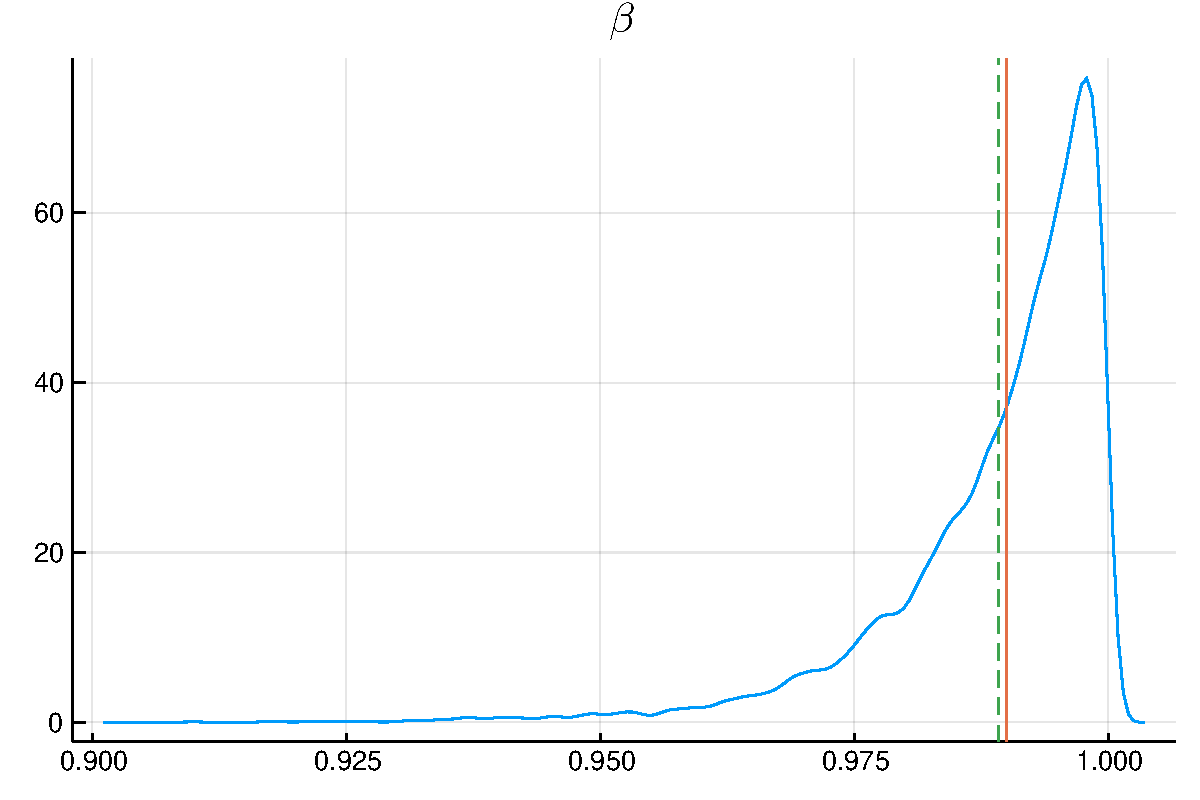
\includegraphics[width=\linewidth]{figures/dsge_and_julia_25_1.pdf}

\begin{lstlisting}
(*@\HLJLn{StatsPlots}@*)(*@\HLJLoB{.}@*)(*@\HLJLnf{density}@*)(*@\HLJLp{(}@*)(*@\HLJLn{pars{\_}convertidos}@*)(*@\HLJLp{[}@*)(*@\HLJLni{50001}@*)(*@\HLJLoB{:}@*)(*@\HLJLni{100000}@*)(*@\HLJLp{,}@*)(*@\HLJLni{2}@*)(*@\HLJLp{],}@*) (*@\HLJLn{legend}@*) (*@\HLJLoB{=:}@*)(*@\HLJLn{none}@*)(*@\HLJLp{)}@*)
(*@\HLJLnf{title!}@*)(*@\HLJLp{(}@*)(*@\HLJLso{L"{}{\textbackslash}epsilon"{}}@*)(*@\HLJLp{)}@*)
(*@\HLJLnf{vline!}@*)(*@\HLJLp{([}@*)(*@\HLJLn{true{\_}pars}@*)(*@\HLJLp{[}@*)(*@\HLJLsc{:epsilon}@*)(*@\HLJLp{]])}@*)
(*@\HLJLnf{vline!}@*)(*@\HLJLp{([}@*)(*@\HLJLnf{mean}@*)(*@\HLJLp{(}@*)(*@\HLJLn{pars{\_}convertidos}@*)(*@\HLJLp{[}@*)(*@\HLJLni{50001}@*)(*@\HLJLoB{:}@*)(*@\HLJLni{100000}@*)(*@\HLJLp{,}@*)(*@\HLJLni{2}@*)(*@\HLJLp{])],}@*) (*@\HLJLn{line}@*) (*@\HLJLoB{=}@*) (*@\HLJLsc{:dash}@*)(*@\HLJLp{)}@*)
\end{lstlisting}

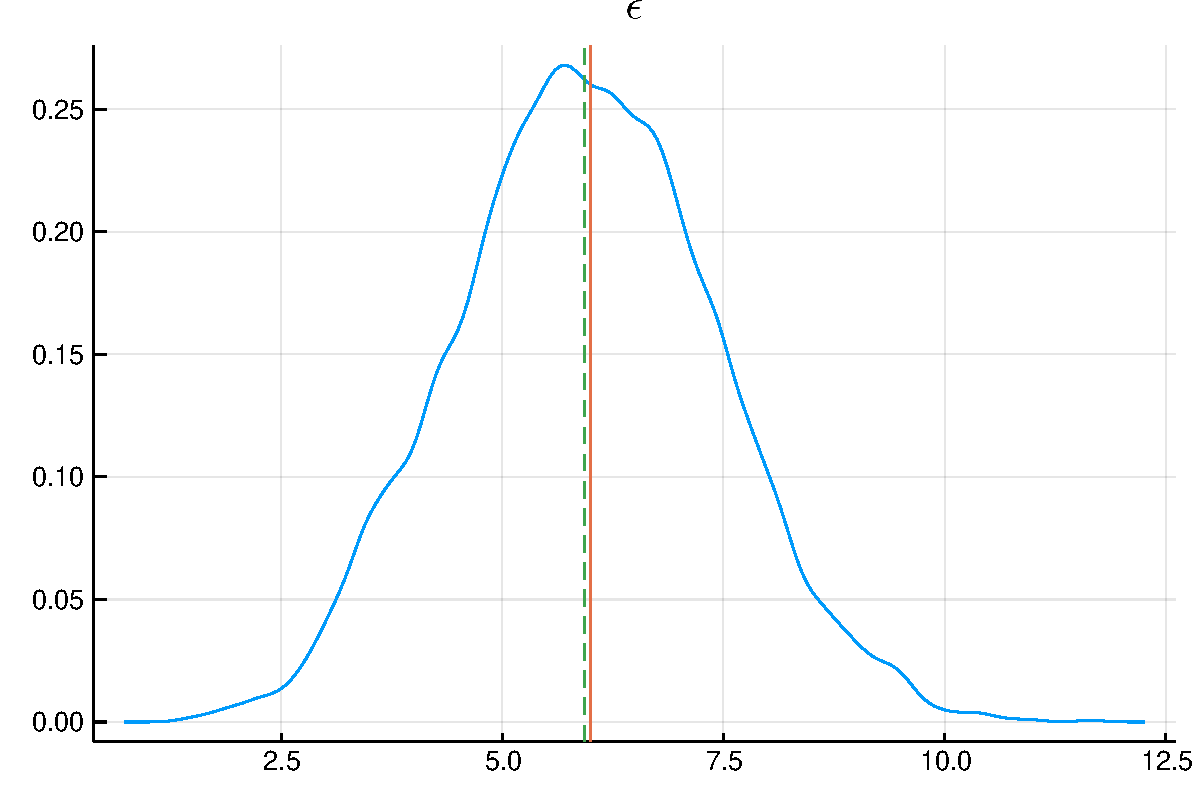
\includegraphics[width=\linewidth]{figures/dsge_and_julia_26_1.pdf}

\begin{lstlisting}
(*@\HLJLn{StatsPlots}@*)(*@\HLJLoB{.}@*)(*@\HLJLnf{density}@*)(*@\HLJLp{(}@*)(*@\HLJLn{pars{\_}convertidos}@*)(*@\HLJLp{[}@*)(*@\HLJLni{50001}@*)(*@\HLJLoB{:}@*)(*@\HLJLni{100000}@*)(*@\HLJLp{,}@*)(*@\HLJLni{3}@*)(*@\HLJLp{],}@*) (*@\HLJLn{legend}@*) (*@\HLJLoB{=}@*) (*@\HLJLsc{:none}@*)(*@\HLJLp{)}@*)
(*@\HLJLnf{title!}@*)(*@\HLJLp{(}@*)(*@\HLJLso{L"{}{\textbackslash}theta"{}}@*)(*@\HLJLp{)}@*)
(*@\HLJLnf{vline!}@*)(*@\HLJLp{([}@*)(*@\HLJLn{true{\_}pars}@*)(*@\HLJLp{[}@*)(*@\HLJLsc{:theta}@*)(*@\HLJLp{]])}@*)
(*@\HLJLnf{vline!}@*)(*@\HLJLp{([}@*)(*@\HLJLnf{mean}@*)(*@\HLJLp{(}@*)(*@\HLJLn{pars{\_}convertidos}@*)(*@\HLJLp{[}@*)(*@\HLJLni{50001}@*)(*@\HLJLoB{:}@*)(*@\HLJLni{100000}@*)(*@\HLJLp{,}@*)(*@\HLJLni{3}@*)(*@\HLJLp{])],}@*) (*@\HLJLn{line}@*) (*@\HLJLoB{=}@*) (*@\HLJLsc{:dash}@*)(*@\HLJLp{)}@*)
\end{lstlisting}

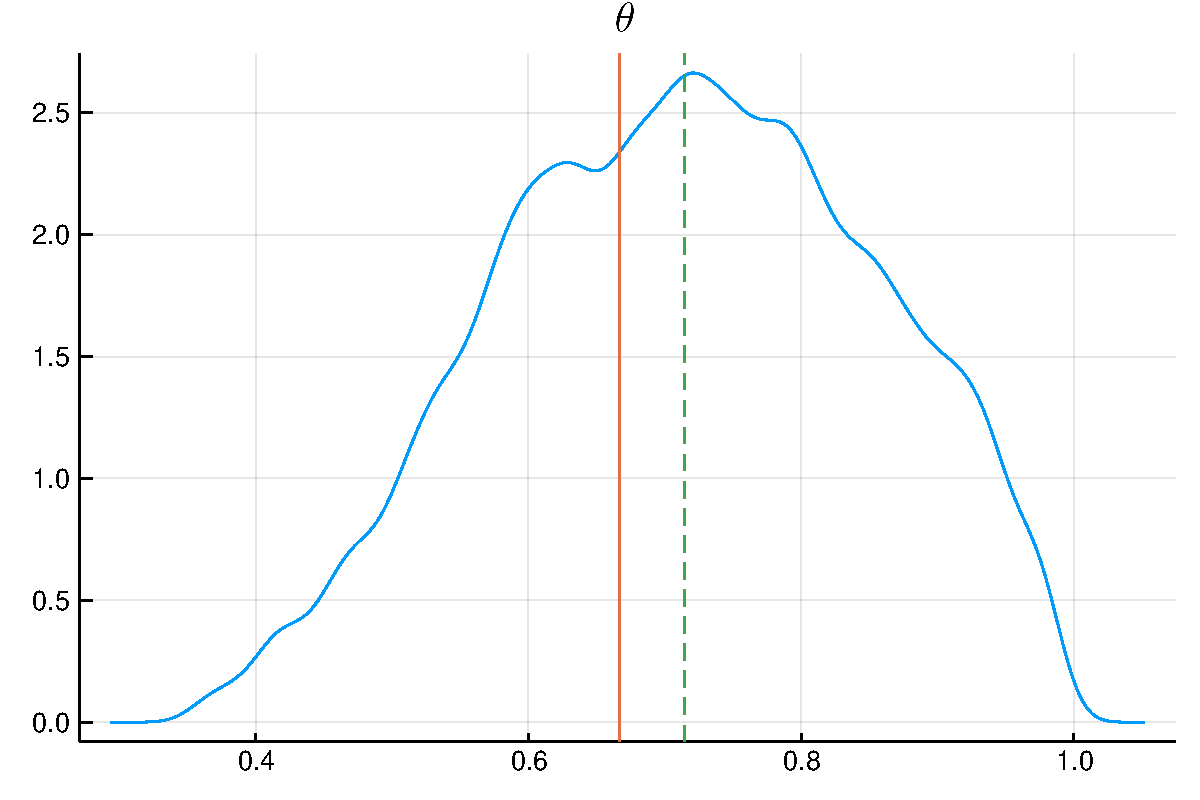
\includegraphics[width=\linewidth]{figures/dsge_and_julia_27_1.pdf}

\begin{lstlisting}
(*@\HLJLn{StatsPlots}@*)(*@\HLJLoB{.}@*)(*@\HLJLnf{density}@*)(*@\HLJLp{(}@*)(*@\HLJLn{pars{\_}convertidos}@*)(*@\HLJLp{[}@*)(*@\HLJLni{50001}@*)(*@\HLJLoB{:}@*)(*@\HLJLni{100000}@*)(*@\HLJLp{,}@*)(*@\HLJLni{4}@*)(*@\HLJLp{],}@*) (*@\HLJLn{legend}@*) (*@\HLJLoB{=}@*) (*@\HLJLsc{:none}@*)(*@\HLJLp{)}@*)
(*@\HLJLnf{title!}@*)(*@\HLJLp{(}@*)(*@\HLJLso{L"{}{\textbackslash}sigma"{}}@*)(*@\HLJLp{)}@*)
(*@\HLJLnf{vline!}@*)(*@\HLJLp{([}@*)(*@\HLJLn{true{\_}pars}@*)(*@\HLJLp{[}@*)(*@\HLJLsc{:sig}@*)(*@\HLJLp{]])}@*)
(*@\HLJLnf{vline!}@*)(*@\HLJLp{([}@*)(*@\HLJLnf{mean}@*)(*@\HLJLp{(}@*)(*@\HLJLn{pars{\_}convertidos}@*)(*@\HLJLp{[}@*)(*@\HLJLni{50001}@*)(*@\HLJLoB{:}@*)(*@\HLJLni{100000}@*)(*@\HLJLp{,}@*)(*@\HLJLni{4}@*)(*@\HLJLp{])],}@*) (*@\HLJLn{line}@*) (*@\HLJLoB{=}@*) (*@\HLJLsc{:dash}@*)(*@\HLJLp{)}@*)
\end{lstlisting}

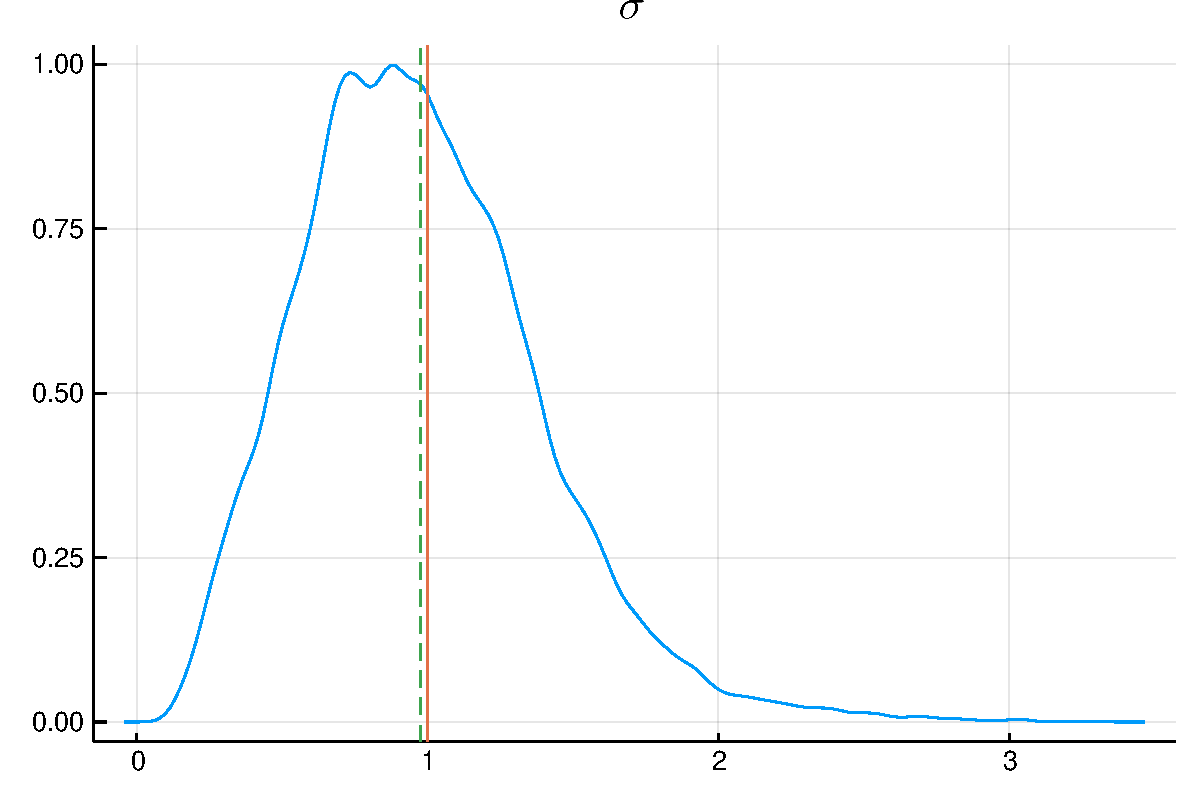
\includegraphics[width=\linewidth]{figures/dsge_and_julia_28_1.pdf}

\begin{lstlisting}
(*@\HLJLn{StatsPlots}@*)(*@\HLJLoB{.}@*)(*@\HLJLnf{density}@*)(*@\HLJLp{(}@*)(*@\HLJLn{pars{\_}convertidos}@*)(*@\HLJLp{[}@*)(*@\HLJLni{50001}@*)(*@\HLJLoB{:}@*)(*@\HLJLni{100000}@*)(*@\HLJLp{,}@*)(*@\HLJLni{5}@*)(*@\HLJLp{],}@*) (*@\HLJLn{legend}@*) (*@\HLJLoB{=}@*) (*@\HLJLsc{:none}@*)(*@\HLJLp{)}@*)
(*@\HLJLnf{title!}@*)(*@\HLJLp{(}@*)(*@\HLJLso{L"{}{\textbackslash}sigma{\textasciicircum}2"{}}@*)(*@\HLJLp{)}@*)
(*@\HLJLnf{vline!}@*)(*@\HLJLp{([}@*)(*@\HLJLn{true{\_}pars}@*)(*@\HLJLp{[}@*)(*@\HLJLsc{:s2}@*)(*@\HLJLp{]])}@*)
(*@\HLJLnf{vline!}@*)(*@\HLJLp{([}@*)(*@\HLJLnf{mean}@*)(*@\HLJLp{(}@*)(*@\HLJLn{pars{\_}convertidos}@*)(*@\HLJLp{[}@*)(*@\HLJLni{50001}@*)(*@\HLJLoB{:}@*)(*@\HLJLni{100000}@*)(*@\HLJLp{,}@*)(*@\HLJLni{5}@*)(*@\HLJLp{])],}@*) (*@\HLJLn{line}@*) (*@\HLJLoB{=}@*) (*@\HLJLsc{:dash}@*)(*@\HLJLp{)}@*)
\end{lstlisting}

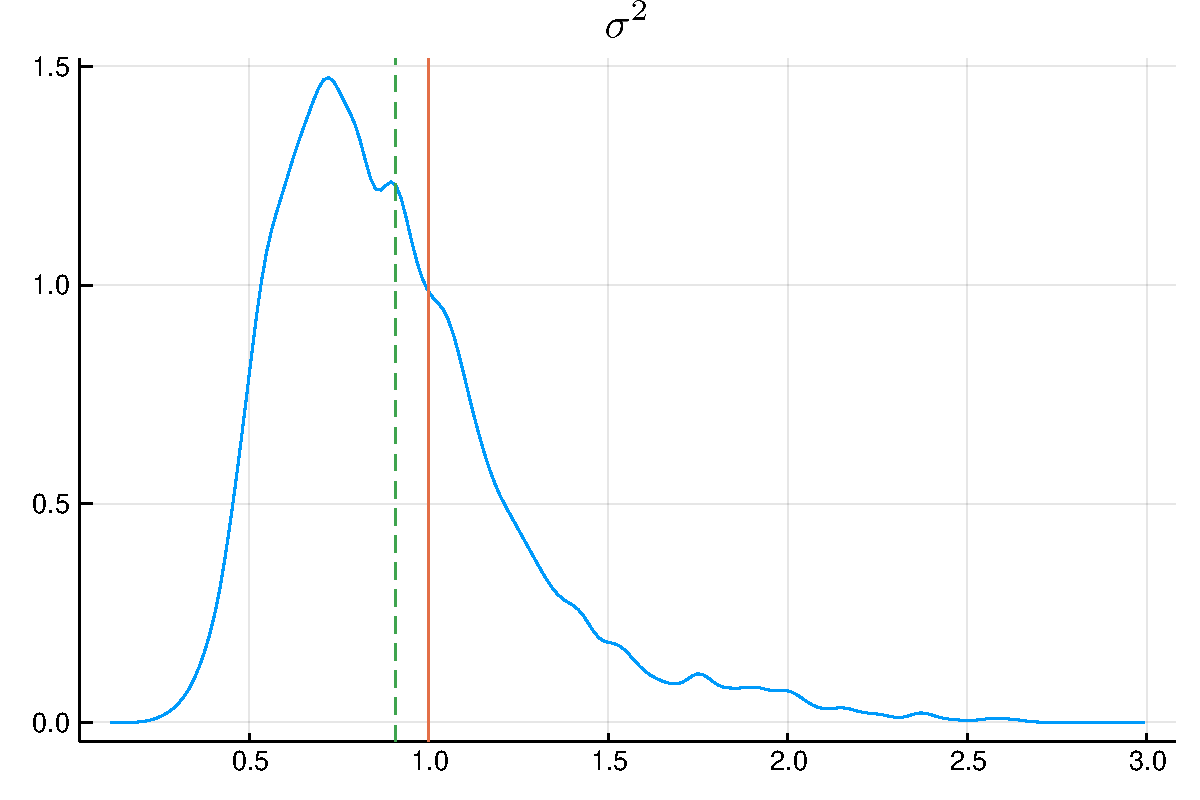
\includegraphics[width=\linewidth]{figures/dsge_and_julia_29_1.pdf}

\begin{lstlisting}
(*@\HLJLn{StatsPlots}@*)(*@\HLJLoB{.}@*)(*@\HLJLnf{density}@*)(*@\HLJLp{(}@*)(*@\HLJLn{pars{\_}convertidos}@*)(*@\HLJLp{[}@*)(*@\HLJLni{50001}@*)(*@\HLJLoB{:}@*)(*@\HLJLni{100000}@*)(*@\HLJLp{,}@*)(*@\HLJLni{6}@*)(*@\HLJLp{],}@*) (*@\HLJLn{legend}@*) (*@\HLJLoB{=}@*) (*@\HLJLsc{:none}@*)(*@\HLJLp{)}@*)
(*@\HLJLnf{title!}@*)(*@\HLJLp{(}@*)(*@\HLJLso{L"{}{\textbackslash}phi"{}}@*)(*@\HLJLp{)}@*)
(*@\HLJLnf{vline!}@*)(*@\HLJLp{([}@*)(*@\HLJLn{true{\_}pars}@*)(*@\HLJLp{[}@*)(*@\HLJLsc{:phi}@*)(*@\HLJLp{]])}@*)
(*@\HLJLnf{vline!}@*)(*@\HLJLp{([}@*)(*@\HLJLnf{mean}@*)(*@\HLJLp{(}@*)(*@\HLJLn{pars{\_}convertidos}@*)(*@\HLJLp{[}@*)(*@\HLJLni{50001}@*)(*@\HLJLoB{:}@*)(*@\HLJLni{100000}@*)(*@\HLJLp{,}@*)(*@\HLJLni{6}@*)(*@\HLJLp{])],}@*) (*@\HLJLn{line}@*) (*@\HLJLoB{=}@*) (*@\HLJLsc{:dash}@*)(*@\HLJLp{)}@*)
\end{lstlisting}

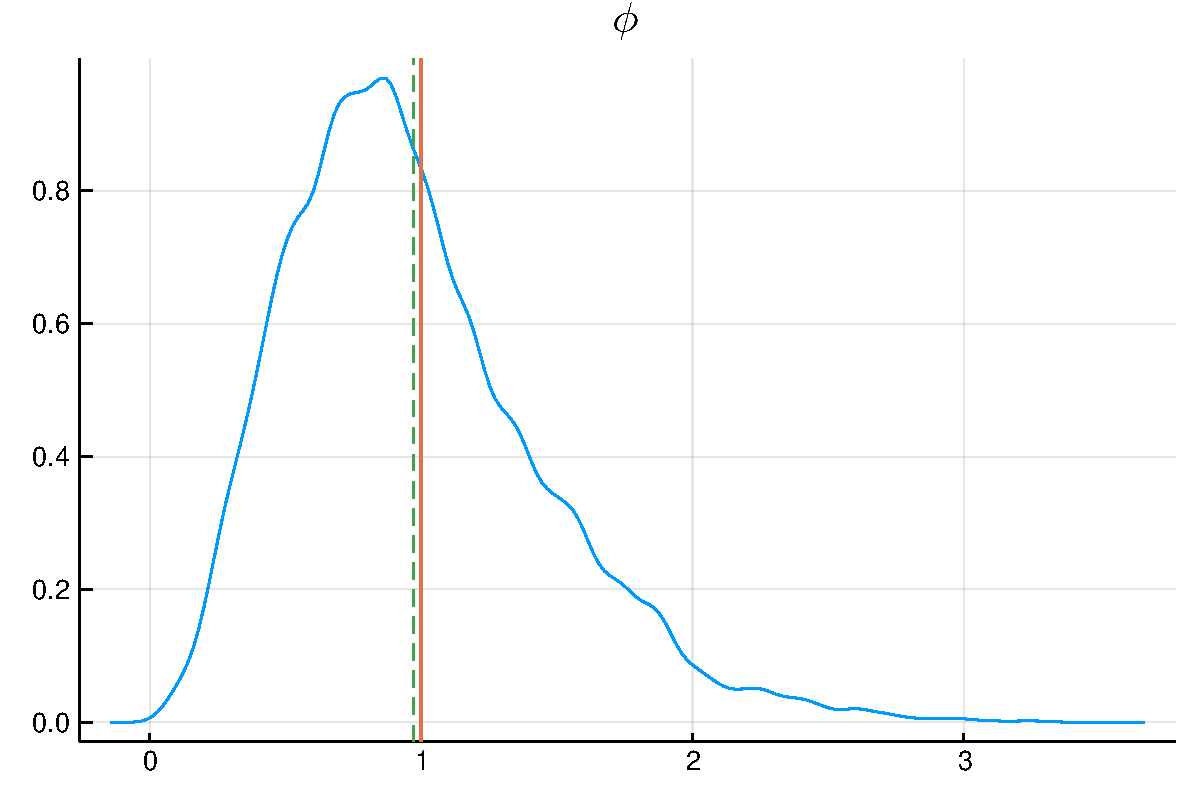
\includegraphics[width=\linewidth]{figures/dsge_and_julia_30_1.pdf}

\begin{lstlisting}
(*@\HLJLn{StatsPlots}@*)(*@\HLJLoB{.}@*)(*@\HLJLnf{density}@*)(*@\HLJLp{(}@*)(*@\HLJLn{pars{\_}convertidos}@*)(*@\HLJLp{[}@*)(*@\HLJLni{50001}@*)(*@\HLJLoB{:}@*)(*@\HLJLni{100000}@*)(*@\HLJLp{,}@*)(*@\HLJLni{7}@*)(*@\HLJLp{],}@*) (*@\HLJLn{legend}@*) (*@\HLJLoB{=}@*) (*@\HLJLsc{:none}@*)(*@\HLJLp{)}@*)
(*@\HLJLnf{title!}@*)(*@\HLJLp{(}@*)(*@\HLJLso{L"{}{\textbackslash}phi{\_}{\{}{\textbackslash}pi{\}}"{}}@*)(*@\HLJLp{)}@*)
(*@\HLJLnf{vline!}@*)(*@\HLJLp{([}@*)(*@\HLJLn{true{\_}pars}@*)(*@\HLJLp{[}@*)(*@\HLJLsc{:phi{\_}pi}@*)(*@\HLJLp{]])}@*)
(*@\HLJLnf{vline!}@*)(*@\HLJLp{([}@*)(*@\HLJLnf{mean}@*)(*@\HLJLp{(}@*)(*@\HLJLn{pars{\_}convertidos}@*)(*@\HLJLp{[}@*)(*@\HLJLni{50001}@*)(*@\HLJLoB{:}@*)(*@\HLJLni{100000}@*)(*@\HLJLp{,}@*)(*@\HLJLni{7}@*)(*@\HLJLp{])],}@*) (*@\HLJLn{line}@*) (*@\HLJLoB{=}@*) (*@\HLJLsc{:dash}@*)(*@\HLJLp{)}@*)
\end{lstlisting}

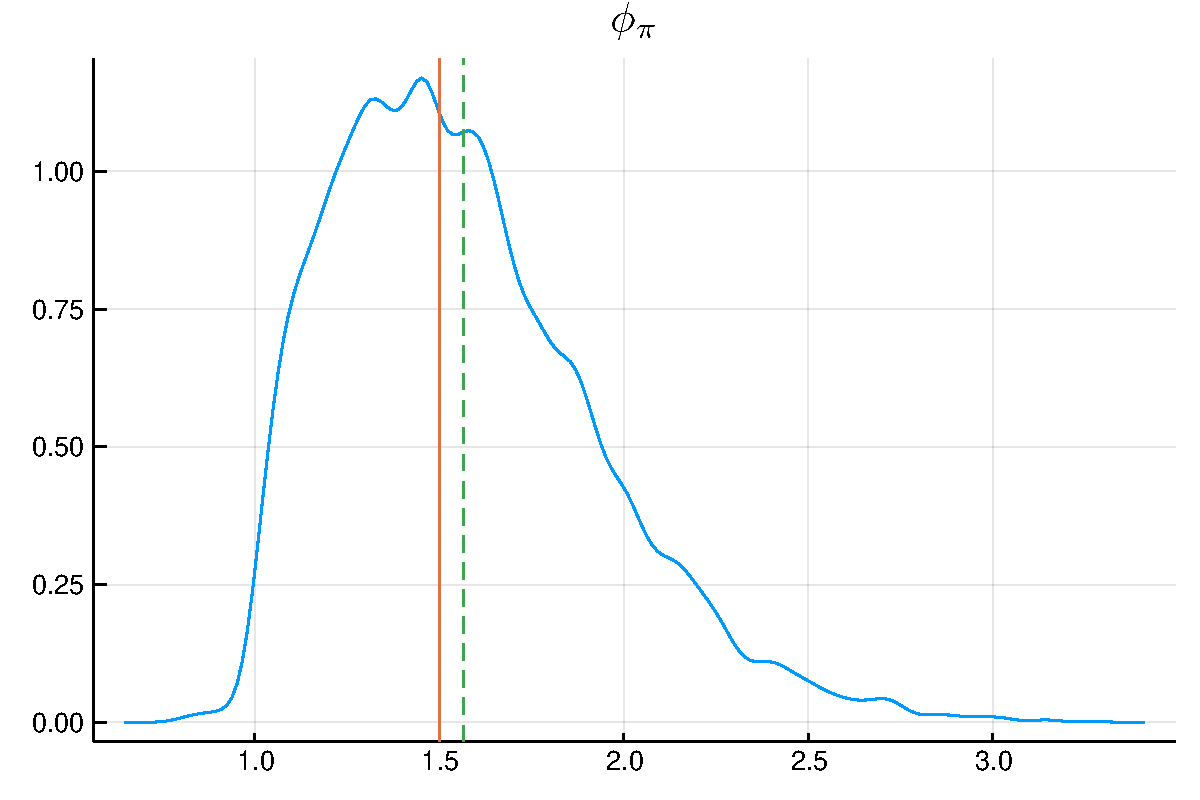
\includegraphics[width=\linewidth]{figures/dsge_and_julia_31_1.pdf}

\begin{lstlisting}
(*@\HLJLn{StatsPlots}@*)(*@\HLJLoB{.}@*)(*@\HLJLnf{density}@*)(*@\HLJLp{(}@*)(*@\HLJLn{pars{\_}convertidos}@*)(*@\HLJLp{[}@*)(*@\HLJLni{50001}@*)(*@\HLJLoB{:}@*)(*@\HLJLni{100000}@*)(*@\HLJLp{,}@*)(*@\HLJLni{8}@*)(*@\HLJLp{],}@*) (*@\HLJLn{legend}@*) (*@\HLJLoB{=}@*) (*@\HLJLsc{:none}@*)(*@\HLJLp{)}@*)
(*@\HLJLnf{title!}@*)(*@\HLJLp{(}@*)(*@\HLJLso{L"{}{\textbackslash}phi{\_}y"{}}@*)(*@\HLJLp{)}@*)
(*@\HLJLnf{vline!}@*)(*@\HLJLp{([}@*)(*@\HLJLn{true{\_}pars}@*)(*@\HLJLp{[}@*)(*@\HLJLsc{:phi{\_}y}@*)(*@\HLJLp{]])}@*)
(*@\HLJLnf{vline!}@*)(*@\HLJLp{([}@*)(*@\HLJLnf{mean}@*)(*@\HLJLp{(}@*)(*@\HLJLn{pars{\_}convertidos}@*)(*@\HLJLp{[}@*)(*@\HLJLni{50001}@*)(*@\HLJLoB{:}@*)(*@\HLJLni{100000}@*)(*@\HLJLp{,}@*)(*@\HLJLni{8}@*)(*@\HLJLp{])],}@*) (*@\HLJLn{line}@*) (*@\HLJLoB{=}@*) (*@\HLJLsc{:dash}@*)(*@\HLJLp{)}@*)
\end{lstlisting}

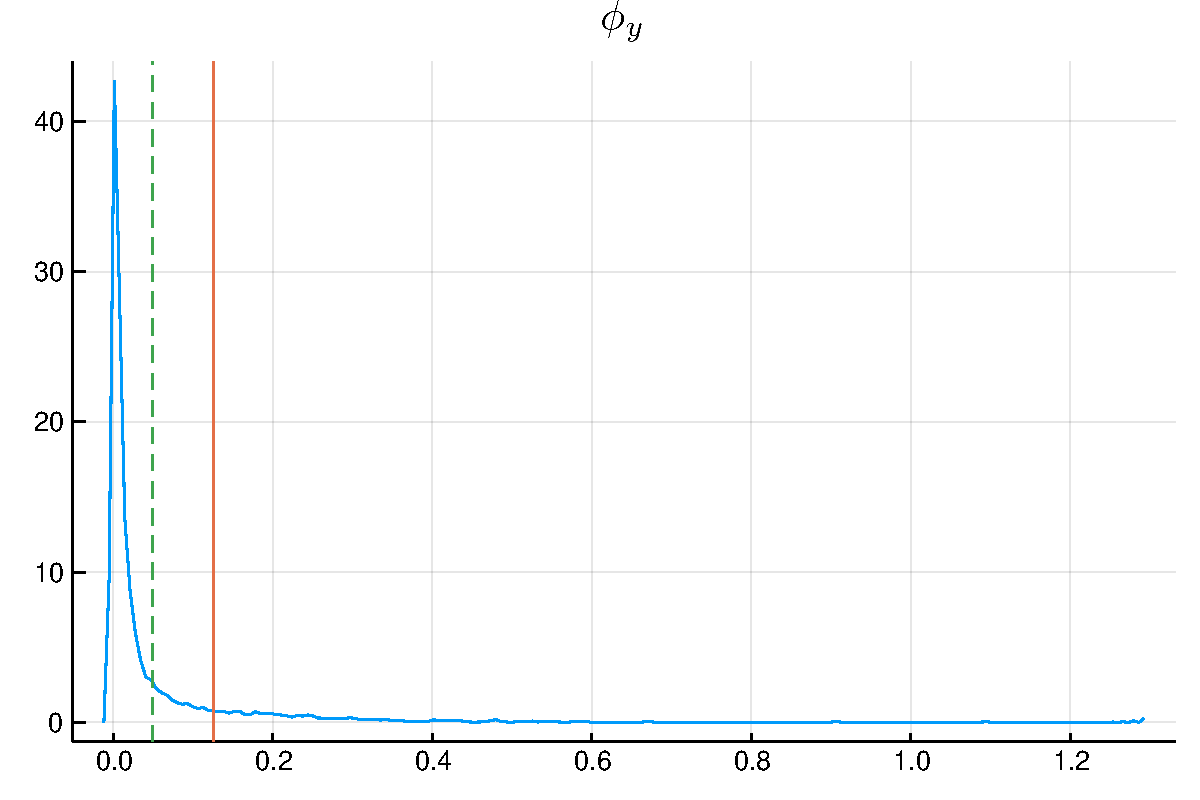
\includegraphics[width=\linewidth]{figures/dsge_and_julia_32_1.pdf}

\begin{lstlisting}
(*@\HLJLn{StatsPlots}@*)(*@\HLJLoB{.}@*)(*@\HLJLnf{density}@*)(*@\HLJLp{(}@*)(*@\HLJLn{pars{\_}convertidos}@*)(*@\HLJLp{[}@*)(*@\HLJLni{50001}@*)(*@\HLJLoB{:}@*)(*@\HLJLni{100000}@*)(*@\HLJLp{,}@*)(*@\HLJLni{9}@*)(*@\HLJLp{],}@*) (*@\HLJLn{legend}@*) (*@\HLJLoB{=}@*) (*@\HLJLsc{:none}@*)(*@\HLJLp{)}@*)
(*@\HLJLnf{title!}@*)(*@\HLJLp{(}@*)(*@\HLJLso{L"{}{\textbackslash}rho{\_}v"{}}@*)(*@\HLJLp{)}@*)
(*@\HLJLnf{vline!}@*)(*@\HLJLp{([}@*)(*@\HLJLn{true{\_}pars}@*)(*@\HLJLp{[}@*)(*@\HLJLsc{:rho{\_}v}@*)(*@\HLJLp{]])}@*)
(*@\HLJLnf{vline!}@*)(*@\HLJLp{([}@*)(*@\HLJLnf{mean}@*)(*@\HLJLp{(}@*)(*@\HLJLn{pars{\_}convertidos}@*)(*@\HLJLp{[}@*)(*@\HLJLni{50001}@*)(*@\HLJLoB{:}@*)(*@\HLJLni{100000}@*)(*@\HLJLp{,}@*)(*@\HLJLni{9}@*)(*@\HLJLp{])],}@*) (*@\HLJLn{line}@*) (*@\HLJLoB{=}@*) (*@\HLJLsc{:dash}@*)(*@\HLJLp{)}@*)
\end{lstlisting}

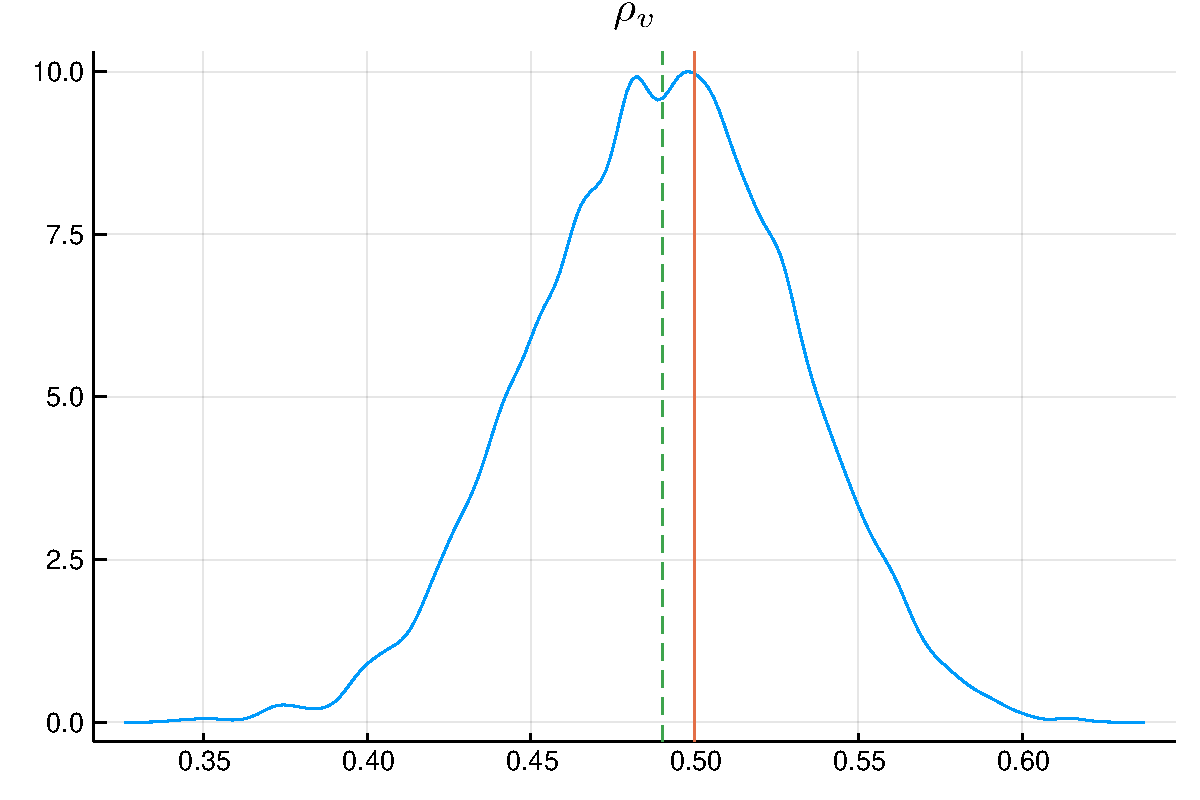
\includegraphics[width=\linewidth]{figures/dsge_and_julia_33_1.pdf}

The algorithm is pretty sucessful. All means are close to the true value and so are the modes. The algorithm has a hard time recovering $\phi_y$; however, it is surprisingly sucessful recovering $\epsilon$, which is inside the expression for $\kappa$.  

\subsection{Hamiltonian Monte Carlo}
Although Random Walk Metropolis Hasting (RWMH) is the main method used when estimating DSGEs by Bayesian methods, it is not the only MCMC algorithm. RWMH is a reliable and relatively simple algorithm to implement, and only requires evaluating the likelihood twice per iteration - which in our case is costly - and does not require knowing the marginal distribution like Gibb's Sampler. However, RWMH relies on a random walk to explore the parametric space: it may wander through regions with low density. This is even worse in high dimensional cases.\cite{Betancourt2017} gives an intuitive example of what goes wrong, using Figure \textbf{????}:

\begin{figure}
\centering
\caption{Changes in volume outside }
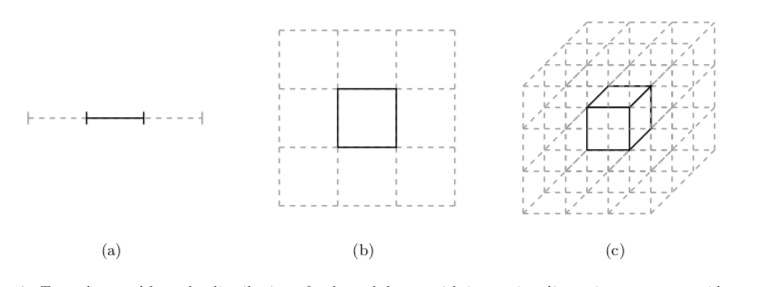
\includegraphics[width=\linewidth]{../3regions.png}
\end{figure}


\cite{Betancourt2017} explains the figure as follows: in one dimension (figure (a)), a division in three parts of the line makes the total mass in the center partition equals 1/3; in $\mathbb{R}^2$ (figure (b)) we have in the center a mass of 1/9; in $\mathbb{R}^3$ (figure (c)), the mass on the center is just 1/27. The volume around the mode is negligible for high dimensional spaces. However, the density function is small outside the region outside mode. this generate a trade off: stay too near to the mode and you will never explore most of the volume; go too far and you will be exploring regions with low density.

The region that we want to explore is called the \emph{typical set}. This is loosely the set that achieves a balance between the two points above, and it has a formal definition in terms of information theory. The problem is that RWMH wanders around the space of parameters and this does not guarantee that it will reach or stay in the typical set in finite time - the time we usually have for simulations.

Fortunately enough, we have a vector that always points toward the mode: the gradient. The Hamiltonian Monte Carlo (HMC) combines this information with the usual Metropolis Hasting algorithm to make sure that the algorithm explores the typical set. \cite{Betancourt2017} uses as a metaphor putting a satellite in orbit: the satellite is attracted to the point with larger mass (the earth). We want our satellite to orbit earth, so we have to give enough impulse that it does not comes crash down on earth; however we don't want to give it \emph{too} much impulse and start wandering around the solar system.

The heart of the Hamiltonian Monte Carlo is to add an additional variable, that is deterministic, that measures the impulse that is given for each parameter. This has to be chosen - as the scale parameter of the RWMH - to guarantee that we will stay in the typical set. This variable follows the dynamics of a Hamiltonian system of physics, which explains the name.

The implementation is not as easy as the RWMH, since we have to keep track of the impulse and update it accordingly the Hamiltonian of the system. Fortunately, there are plenty of implementations of HMC in Julia. We will use the package \textbf{DynamicHMC}, that follows the implementation suggested in Bethancourt's paper. We have to give to it the (numerator of) the posterior and it's gradient, and the package does everything else.

Getting the gradient is tricky. \cite{Gelman2014} explicitly acknowledge that "In practice the gradient must be computed analytically; numerical differentiation requires too many function evaluations to be computed analytically". It is hard to imagine \emph{how} to compute the analytical derivate of each parameter, given the amount of computations that go into building the likelihood. Therefore, we have to rely on numerical differentiation. The usual method for differentiating, finite difference, requires a lot of function evaluation (at least two for each variable) and is prone to numerical errors - which can only be reduced by evaluating the function even more times. A first attempt using finite differences led to a running time of at least 12 hours.

However, there are better methods than finite differences. One of them is automatic differentiation. Although it builds from dual numbers and other concepts of algebra, that is not a subject usually dealt by economists, the idea is just to use the chain rule: to differentiate a given function, differentiate each component that forms the function. This is both faster and more precise than finite differences and is implemented by a variety of packages in Julia. We use \textbf{Tracker}: some other packages for automatic differentiation do not differentiate over the Schur decomposition.

The code that estimates the DSGE using the likelihood we built above is:



\begin{lstlisting}
(*@\HLJLk{using}@*) (*@\HLJLn{Tracker}@*)(*@\HLJLp{,}@*) (*@\HLJLn{DynamicHMC}@*)

(*@\HLJLn{grad{\_}p}@*) (*@\HLJLoB{=}@*) (*@\HLJLnf{ADgradient}@*)(*@\HLJLp{(}@*)(*@\HLJLsc{:Tracker}@*)(*@\HLJLp{,}@*)(*@\HLJLn{P}@*)(*@\HLJLp{)}@*)

(*@\HLJLn{res}@*) (*@\HLJLoB{=}@*) (*@\HLJLnf{mcmc{\_}with{\_}warmup}@*)(*@\HLJLp{(}@*)(*@\HLJLn{Random}@*)(*@\HLJLoB{.}@*)(*@\HLJLn{GLOBAL{\_}RNG}@*)(*@\HLJLp{,}@*) (*@\HLJLn{grad{\_}p}@*)(*@\HLJLp{,}@*)(*@\HLJLni{100000}@*)(*@\HLJLp{)}@*)
\end{lstlisting}

And let's show the densities:


\begin{lstlisting}
(*@\HLJLn{pars{\_}hmc}@*) (*@\HLJLoB{=}@*) (*@\HLJLnf{load}@*)(*@\HLJLp{(}@*)(*@\HLJLs{"{}data/hmc2.jld"{}}@*)(*@\HLJLp{)[}@*)(*@\HLJLs{"{}pars"{}}@*)(*@\HLJLp{]}@*)

(*@\HLJLn{StatsPlots}@*)(*@\HLJLoB{.}@*)(*@\HLJLnf{density}@*)(*@\HLJLp{(}@*)(*@\HLJLn{pars{\_}hmc}@*)(*@\HLJLp{[}@*)(*@\HLJLoB{:}@*)(*@\HLJLp{,}@*)(*@\HLJLni{1}@*)(*@\HLJLp{],}@*) (*@\HLJLn{legend}@*) (*@\HLJLoB{=:}@*)(*@\HLJLn{none}@*)(*@\HLJLp{)}@*)
(*@\HLJLnf{title!}@*)(*@\HLJLp{(}@*)(*@\HLJLso{L"{}{\textbackslash}beta"{}}@*)(*@\HLJLp{)}@*)
(*@\HLJLnf{vline!}@*)(*@\HLJLp{([}@*)(*@\HLJLn{true{\_}pars}@*)(*@\HLJLp{[}@*)(*@\HLJLsc{:bet}@*)(*@\HLJLp{]])}@*)
(*@\HLJLnf{vline!}@*)(*@\HLJLp{([}@*)(*@\HLJLnf{mean}@*)(*@\HLJLp{(}@*)(*@\HLJLn{pars{\_}hmc}@*)(*@\HLJLp{[}@*)(*@\HLJLoB{:}@*)(*@\HLJLp{,}@*)(*@\HLJLni{1}@*)(*@\HLJLp{])],}@*) (*@\HLJLn{line}@*) (*@\HLJLoB{=}@*) (*@\HLJLsc{:dash}@*)(*@\HLJLp{)}@*)
\end{lstlisting}

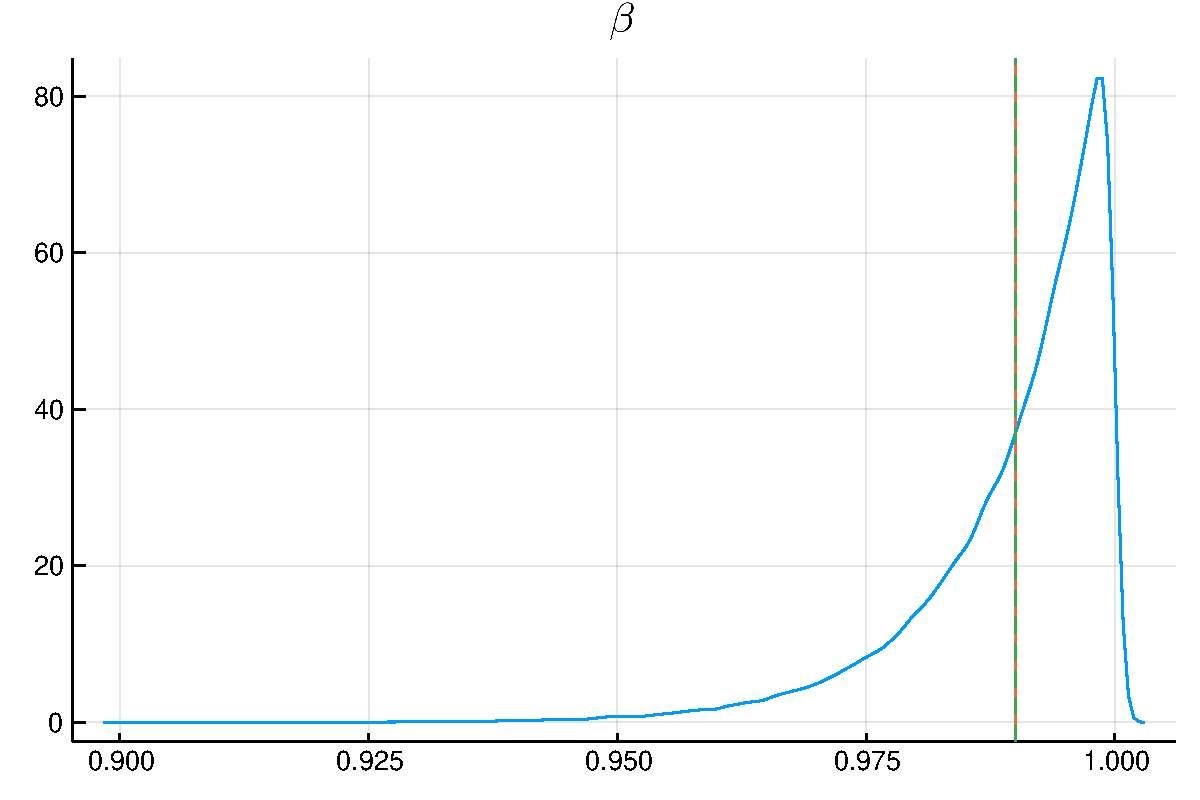
\includegraphics[width=\linewidth]{figures/dsge_and_julia_35_1.pdf}

\begin{lstlisting}
(*@\HLJLn{StatsPlots}@*)(*@\HLJLoB{.}@*)(*@\HLJLnf{density}@*)(*@\HLJLp{(}@*)(*@\HLJLn{pars{\_}hmc}@*)(*@\HLJLp{[}@*)(*@\HLJLoB{:}@*)(*@\HLJLp{,}@*)(*@\HLJLni{2}@*)(*@\HLJLp{],}@*) (*@\HLJLn{legend}@*) (*@\HLJLoB{=:}@*)(*@\HLJLn{none}@*)(*@\HLJLp{)}@*)
(*@\HLJLnf{title!}@*)(*@\HLJLp{(}@*)(*@\HLJLso{L"{}{\textbackslash}epsilon"{}}@*)(*@\HLJLp{)}@*)
(*@\HLJLnf{vline!}@*)(*@\HLJLp{([}@*)(*@\HLJLn{true{\_}pars}@*)(*@\HLJLp{[}@*)(*@\HLJLsc{:epsilon}@*)(*@\HLJLp{]])}@*)
(*@\HLJLnf{vline!}@*)(*@\HLJLp{([}@*)(*@\HLJLnf{mean}@*)(*@\HLJLp{(}@*)(*@\HLJLn{pars{\_}hmc}@*)(*@\HLJLp{[}@*)(*@\HLJLoB{:}@*)(*@\HLJLp{,}@*)(*@\HLJLni{2}@*)(*@\HLJLp{])],}@*) (*@\HLJLn{line}@*) (*@\HLJLoB{=}@*) (*@\HLJLsc{:dash}@*)(*@\HLJLp{)}@*)
\end{lstlisting}

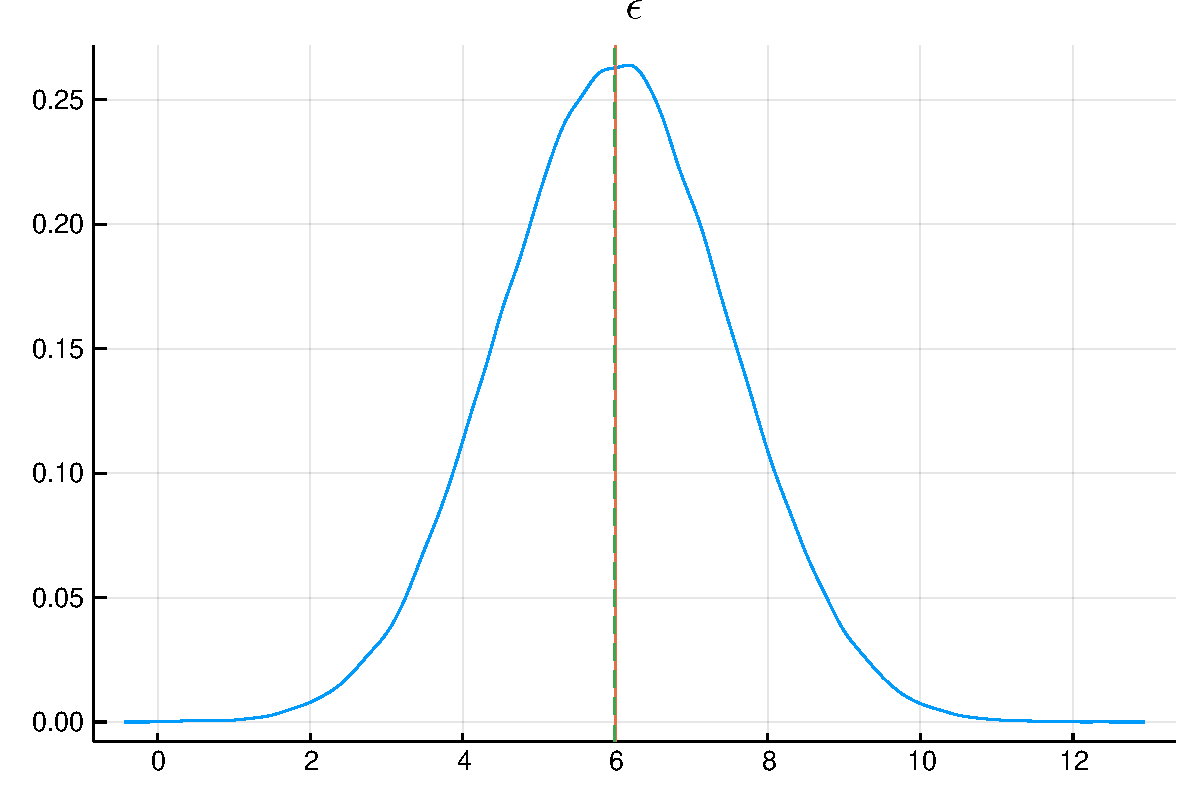
\includegraphics[width=\linewidth]{figures/dsge_and_julia_36_1.pdf}

\begin{lstlisting}
(*@\HLJLn{StatsPlots}@*)(*@\HLJLoB{.}@*)(*@\HLJLnf{density}@*)(*@\HLJLp{(}@*)(*@\HLJLn{pars{\_}hmc}@*)(*@\HLJLp{[}@*)(*@\HLJLoB{:}@*)(*@\HLJLp{,}@*)(*@\HLJLni{3}@*)(*@\HLJLp{],}@*) (*@\HLJLn{legend}@*) (*@\HLJLoB{=:}@*)(*@\HLJLn{none}@*)(*@\HLJLp{)}@*)
(*@\HLJLnf{title!}@*)(*@\HLJLp{(}@*)(*@\HLJLso{L"{}{\textbackslash}theta"{}}@*)(*@\HLJLp{)}@*)
(*@\HLJLnf{vline!}@*)(*@\HLJLp{([}@*)(*@\HLJLn{true{\_}pars}@*)(*@\HLJLp{[}@*)(*@\HLJLsc{:theta}@*)(*@\HLJLp{]])}@*)
(*@\HLJLnf{vline!}@*)(*@\HLJLp{([}@*)(*@\HLJLnf{mean}@*)(*@\HLJLp{(}@*)(*@\HLJLn{pars{\_}hmc}@*)(*@\HLJLp{[}@*)(*@\HLJLoB{:}@*)(*@\HLJLp{,}@*)(*@\HLJLni{3}@*)(*@\HLJLp{])],}@*) (*@\HLJLn{line}@*) (*@\HLJLoB{=}@*) (*@\HLJLsc{:dash}@*)(*@\HLJLp{)}@*)
\end{lstlisting}

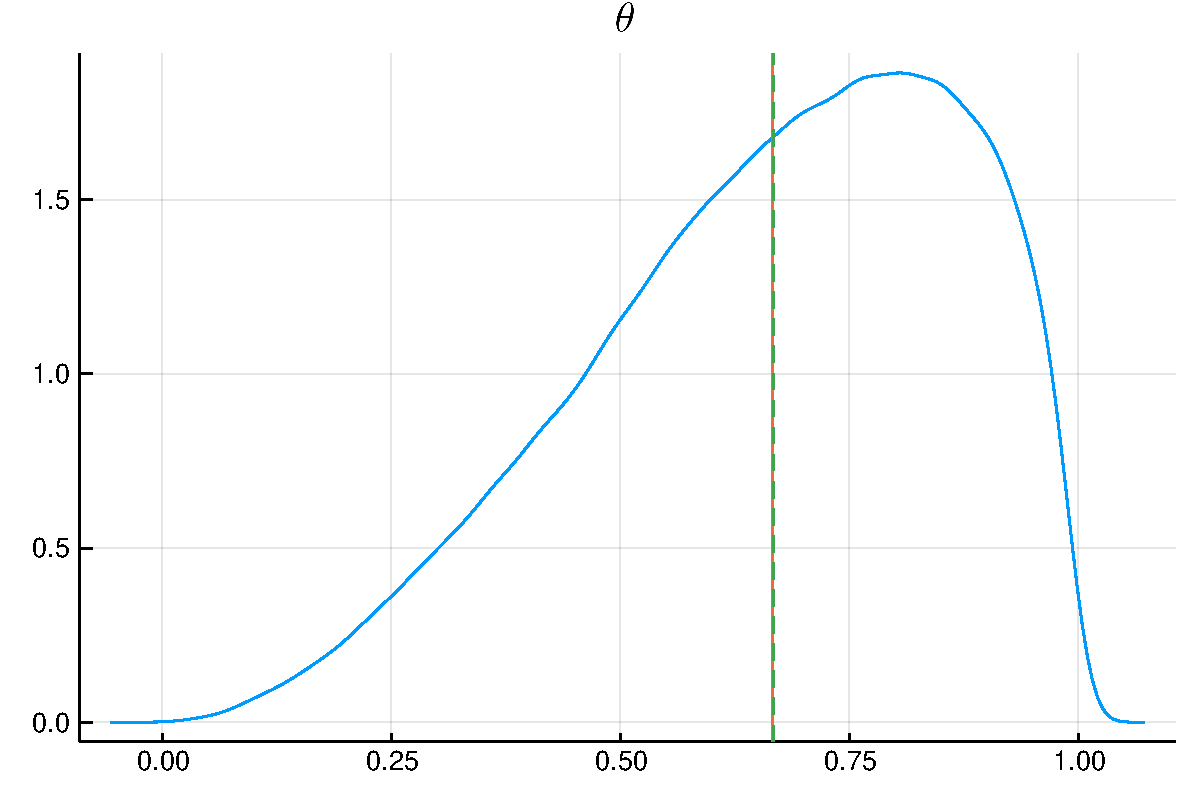
\includegraphics[width=\linewidth]{figures/dsge_and_julia_37_1.pdf}

\begin{lstlisting}
(*@\HLJLn{StatsPlots}@*)(*@\HLJLoB{.}@*)(*@\HLJLnf{density}@*)(*@\HLJLp{(}@*)(*@\HLJLn{pars{\_}hmc}@*)(*@\HLJLp{[}@*)(*@\HLJLoB{:}@*)(*@\HLJLp{,}@*)(*@\HLJLni{4}@*)(*@\HLJLp{],}@*) (*@\HLJLn{legend}@*) (*@\HLJLoB{=:}@*)(*@\HLJLn{none}@*)(*@\HLJLp{)}@*)
(*@\HLJLnf{title!}@*)(*@\HLJLp{(}@*)(*@\HLJLso{L"{}{\textbackslash}sigma"{}}@*)(*@\HLJLp{)}@*)
(*@\HLJLnf{vline!}@*)(*@\HLJLp{([}@*)(*@\HLJLn{true{\_}pars}@*)(*@\HLJLp{[}@*)(*@\HLJLsc{:sig}@*)(*@\HLJLp{]])}@*)
(*@\HLJLnf{vline!}@*)(*@\HLJLp{([}@*)(*@\HLJLnf{mean}@*)(*@\HLJLp{(}@*)(*@\HLJLn{pars{\_}hmc}@*)(*@\HLJLp{[}@*)(*@\HLJLoB{:}@*)(*@\HLJLp{,}@*)(*@\HLJLni{4}@*)(*@\HLJLp{])],}@*) (*@\HLJLn{line}@*) (*@\HLJLoB{=}@*) (*@\HLJLsc{:dash}@*)(*@\HLJLp{)}@*)
\end{lstlisting}

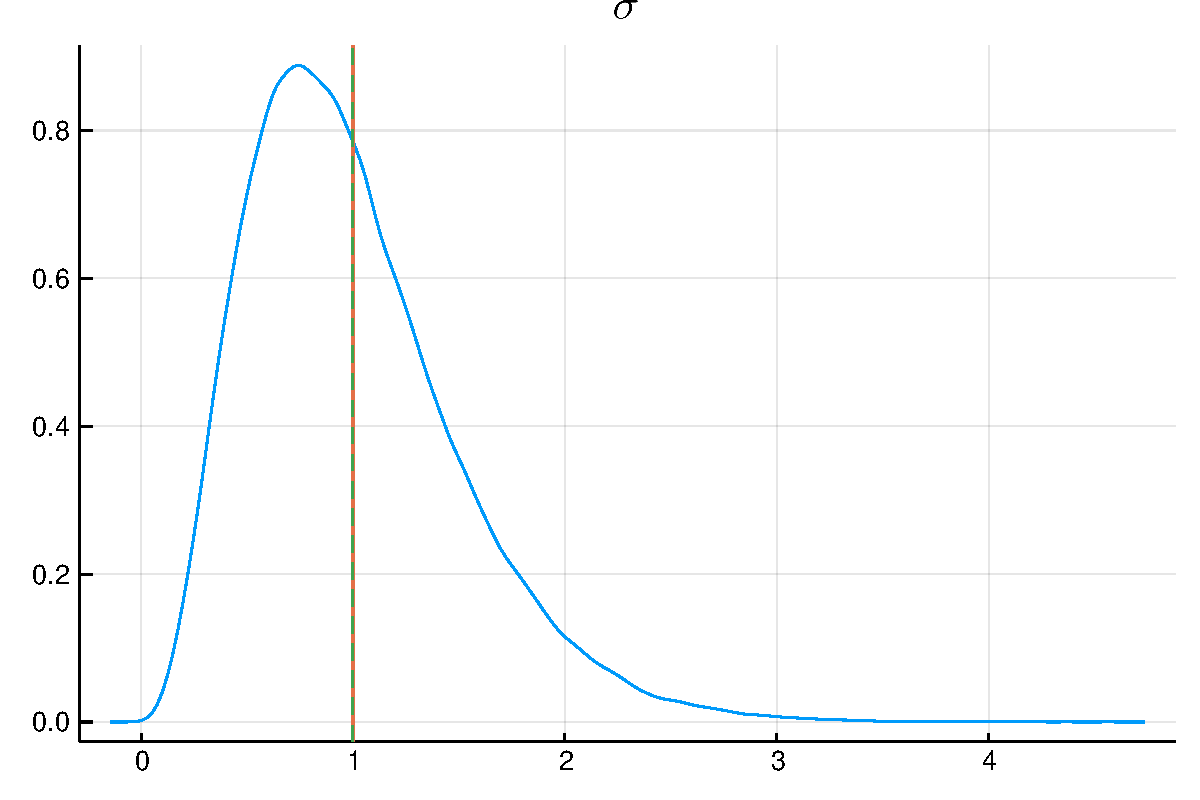
\includegraphics[width=\linewidth]{figures/dsge_and_julia_38_1.pdf}

\begin{lstlisting}
(*@\HLJLn{StatsPlots}@*)(*@\HLJLoB{.}@*)(*@\HLJLnf{density}@*)(*@\HLJLp{(}@*)(*@\HLJLn{pars{\_}hmc}@*)(*@\HLJLp{[}@*)(*@\HLJLoB{:}@*)(*@\HLJLp{,}@*)(*@\HLJLni{5}@*)(*@\HLJLp{],}@*) (*@\HLJLn{legend}@*) (*@\HLJLoB{=:}@*)(*@\HLJLn{none}@*)(*@\HLJLp{)}@*)
(*@\HLJLnf{title!}@*)(*@\HLJLp{(}@*)(*@\HLJLso{L"{}{\textbackslash}sigma{\textasciicircum}2"{}}@*)(*@\HLJLp{)}@*)
(*@\HLJLnf{vline!}@*)(*@\HLJLp{([}@*)(*@\HLJLn{true{\_}pars}@*)(*@\HLJLp{[}@*)(*@\HLJLsc{:s2}@*)(*@\HLJLp{]])}@*)
(*@\HLJLnf{vline!}@*)(*@\HLJLp{([}@*)(*@\HLJLnf{mean}@*)(*@\HLJLp{(}@*)(*@\HLJLn{pars{\_}hmc}@*)(*@\HLJLp{[}@*)(*@\HLJLoB{:}@*)(*@\HLJLp{,}@*)(*@\HLJLni{5}@*)(*@\HLJLp{])],}@*) (*@\HLJLn{line}@*) (*@\HLJLoB{=}@*) (*@\HLJLsc{:dash}@*)(*@\HLJLp{)}@*)
\end{lstlisting}

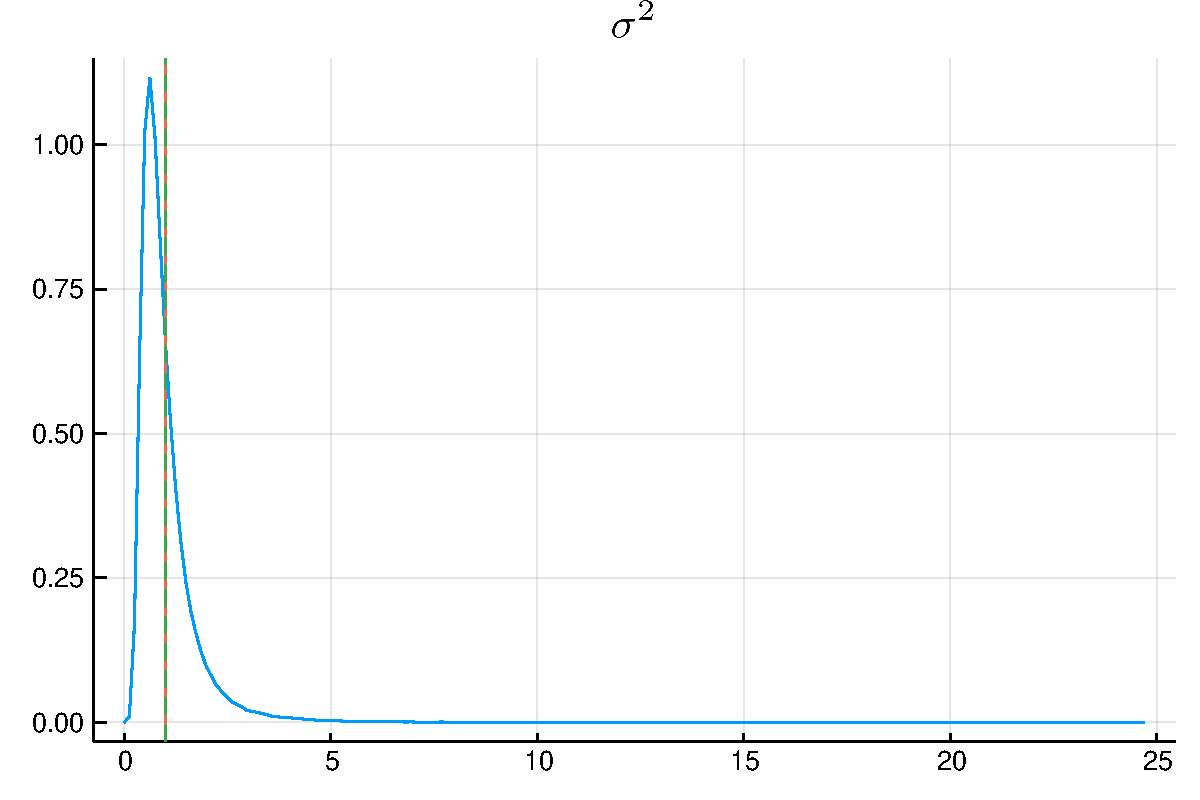
\includegraphics[width=\linewidth]{figures/dsge_and_julia_39_1.pdf}

\begin{lstlisting}
(*@\HLJLn{StatsPlots}@*)(*@\HLJLoB{.}@*)(*@\HLJLnf{density}@*)(*@\HLJLp{(}@*)(*@\HLJLn{pars{\_}hmc}@*)(*@\HLJLp{[}@*)(*@\HLJLoB{:}@*)(*@\HLJLp{,}@*)(*@\HLJLni{6}@*)(*@\HLJLp{],}@*) (*@\HLJLn{legend}@*) (*@\HLJLoB{=:}@*)(*@\HLJLn{none}@*)(*@\HLJLp{)}@*)
(*@\HLJLnf{title!}@*)(*@\HLJLp{(}@*)(*@\HLJLso{L"{}{\textbackslash}phi"{}}@*)(*@\HLJLp{)}@*)
(*@\HLJLnf{vline!}@*)(*@\HLJLp{([}@*)(*@\HLJLn{true{\_}pars}@*)(*@\HLJLp{[}@*)(*@\HLJLsc{:phi}@*)(*@\HLJLp{]])}@*)
(*@\HLJLnf{vline!}@*)(*@\HLJLp{([}@*)(*@\HLJLnf{mean}@*)(*@\HLJLp{(}@*)(*@\HLJLn{pars{\_}hmc}@*)(*@\HLJLp{[}@*)(*@\HLJLoB{:}@*)(*@\HLJLp{,}@*)(*@\HLJLni{6}@*)(*@\HLJLp{])],}@*) (*@\HLJLn{line}@*) (*@\HLJLoB{=}@*) (*@\HLJLsc{:dash}@*)(*@\HLJLp{)}@*)
\end{lstlisting}

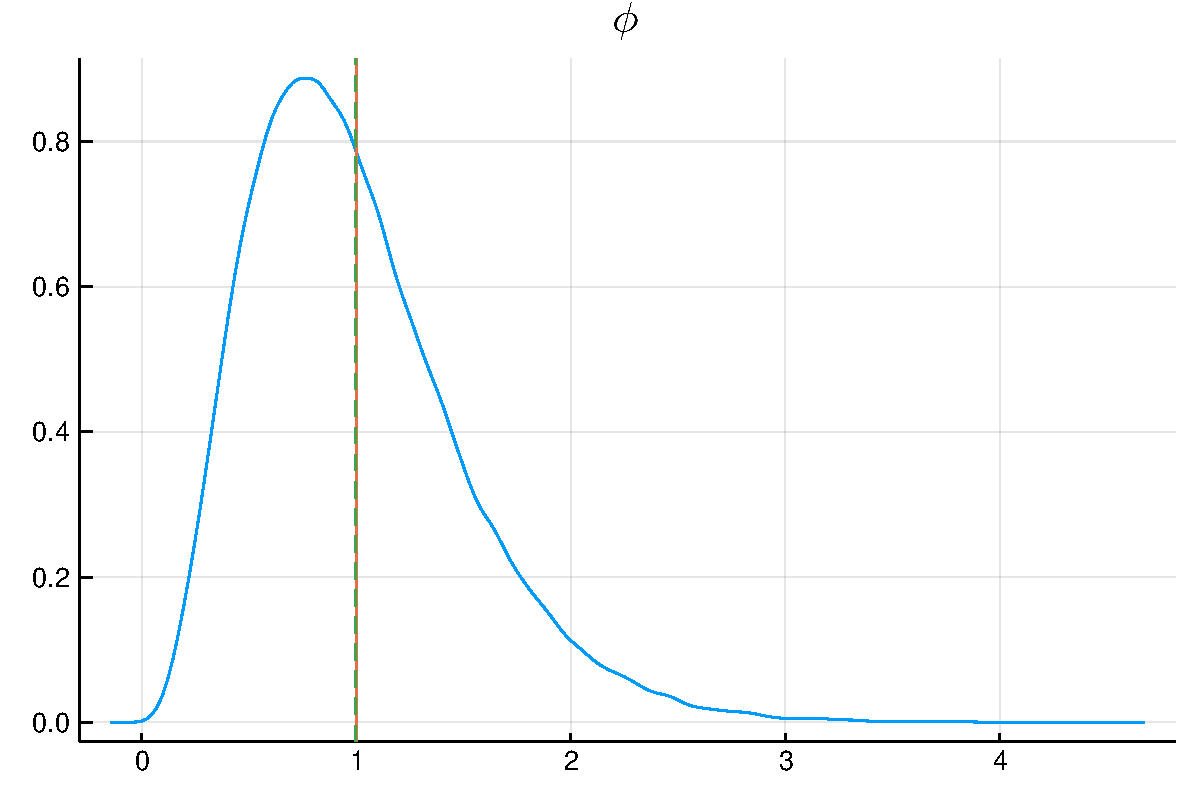
\includegraphics[width=\linewidth]{figures/dsge_and_julia_40_1.pdf}

\begin{lstlisting}
(*@\HLJLn{StatsPlots}@*)(*@\HLJLoB{.}@*)(*@\HLJLnf{density}@*)(*@\HLJLp{(}@*)(*@\HLJLn{pars{\_}hmc}@*)(*@\HLJLp{[}@*)(*@\HLJLoB{:}@*)(*@\HLJLp{,}@*)(*@\HLJLni{7}@*)(*@\HLJLp{],}@*) (*@\HLJLn{legend}@*) (*@\HLJLoB{=:}@*)(*@\HLJLn{none}@*)(*@\HLJLp{)}@*)
(*@\HLJLnf{title!}@*)(*@\HLJLp{(}@*)(*@\HLJLso{L"{}{\textbackslash}phi{\_}{\{}{\textbackslash}pi{\}}"{}}@*)(*@\HLJLp{)}@*)
(*@\HLJLnf{vline!}@*)(*@\HLJLp{([}@*)(*@\HLJLn{true{\_}pars}@*)(*@\HLJLp{[}@*)(*@\HLJLsc{:phi{\_}pi}@*)(*@\HLJLp{]])}@*)
(*@\HLJLnf{vline!}@*)(*@\HLJLp{([}@*)(*@\HLJLnf{mean}@*)(*@\HLJLp{(}@*)(*@\HLJLn{pars{\_}hmc}@*)(*@\HLJLp{[}@*)(*@\HLJLoB{:}@*)(*@\HLJLp{,}@*)(*@\HLJLni{7}@*)(*@\HLJLp{])],}@*) (*@\HLJLn{line}@*) (*@\HLJLoB{=}@*) (*@\HLJLsc{:dash}@*)(*@\HLJLp{)}@*)
\end{lstlisting}

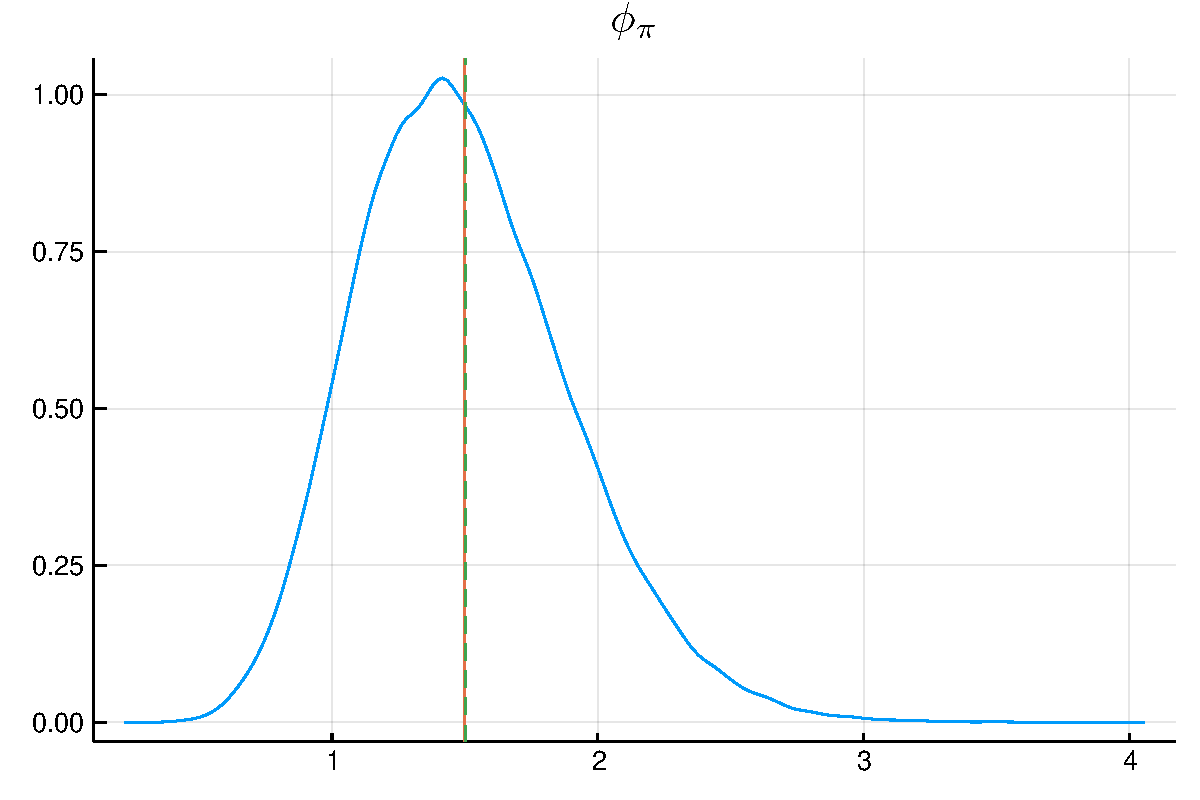
\includegraphics[width=\linewidth]{figures/dsge_and_julia_41_1.pdf}

\begin{lstlisting}
(*@\HLJLn{StatsPlots}@*)(*@\HLJLoB{.}@*)(*@\HLJLnf{density}@*)(*@\HLJLp{(}@*)(*@\HLJLn{pars{\_}hmc}@*)(*@\HLJLp{[}@*)(*@\HLJLoB{:}@*)(*@\HLJLp{,}@*)(*@\HLJLni{8}@*)(*@\HLJLp{],}@*) (*@\HLJLn{legend}@*) (*@\HLJLoB{=:}@*)(*@\HLJLn{none}@*)(*@\HLJLp{)}@*)
(*@\HLJLnf{title!}@*)(*@\HLJLp{(}@*)(*@\HLJLso{L"{}{\textbackslash}phi{\_}y"{}}@*)(*@\HLJLp{)}@*)
(*@\HLJLnf{vline!}@*)(*@\HLJLp{([}@*)(*@\HLJLn{true{\_}pars}@*)(*@\HLJLp{[}@*)(*@\HLJLsc{:phi{\_}y}@*)(*@\HLJLp{]])}@*)
(*@\HLJLnf{vline!}@*)(*@\HLJLp{([}@*)(*@\HLJLnf{mean}@*)(*@\HLJLp{(}@*)(*@\HLJLn{pars{\_}hmc}@*)(*@\HLJLp{[}@*)(*@\HLJLoB{:}@*)(*@\HLJLp{,}@*)(*@\HLJLni{8}@*)(*@\HLJLp{])],}@*) (*@\HLJLn{line}@*) (*@\HLJLoB{=}@*) (*@\HLJLsc{:dash}@*)(*@\HLJLp{)}@*)
\end{lstlisting}

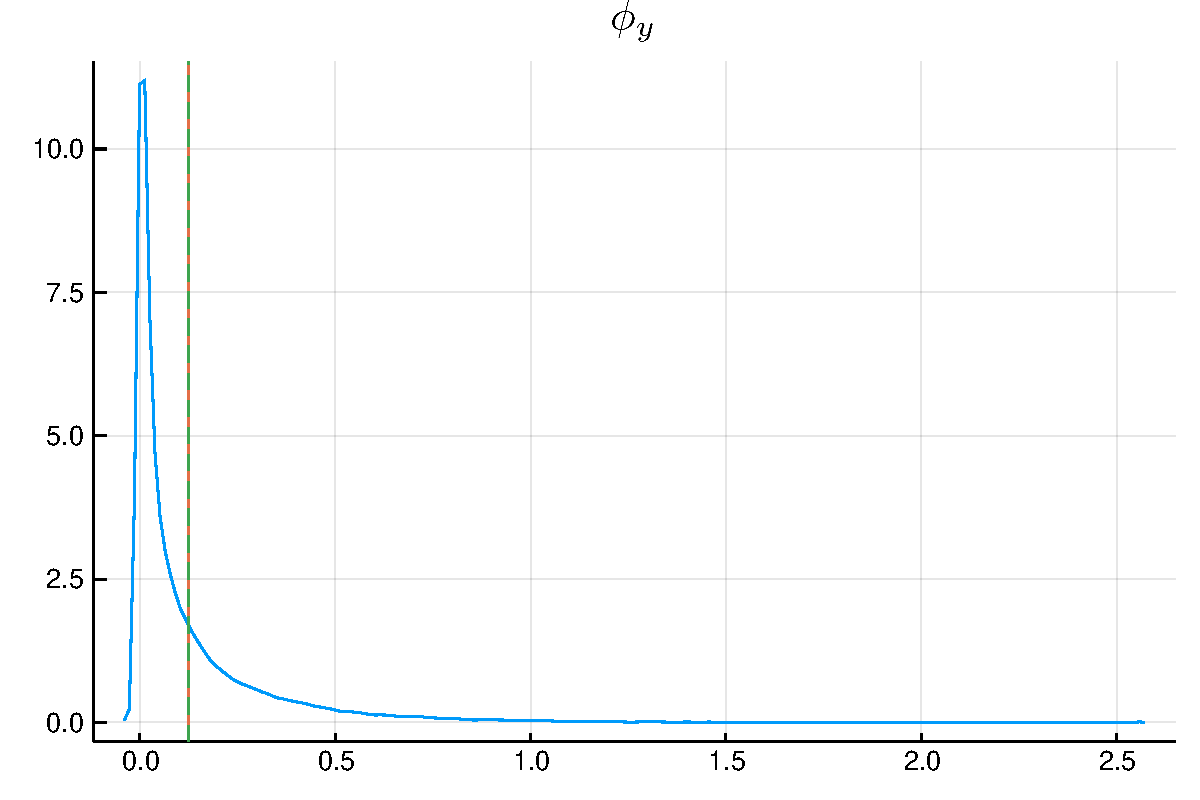
\includegraphics[width=\linewidth]{figures/dsge_and_julia_42_1.pdf}

\begin{lstlisting}
(*@\HLJLn{StatsPlots}@*)(*@\HLJLoB{.}@*)(*@\HLJLnf{density}@*)(*@\HLJLp{(}@*)(*@\HLJLn{pars{\_}hmc}@*)(*@\HLJLp{[}@*)(*@\HLJLoB{:}@*)(*@\HLJLp{,}@*)(*@\HLJLni{9}@*)(*@\HLJLp{],}@*) (*@\HLJLn{legend}@*) (*@\HLJLoB{=:}@*)(*@\HLJLn{none}@*)(*@\HLJLp{)}@*)
(*@\HLJLnf{title!}@*)(*@\HLJLp{(}@*)(*@\HLJLso{L"{}{\textbackslash}rho{\_}v"{}}@*)(*@\HLJLp{)}@*)
(*@\HLJLnf{vline!}@*)(*@\HLJLp{([}@*)(*@\HLJLn{true{\_}pars}@*)(*@\HLJLp{[}@*)(*@\HLJLsc{:rho{\_}v}@*)(*@\HLJLp{]])}@*)
(*@\HLJLnf{vline!}@*)(*@\HLJLp{([}@*)(*@\HLJLnf{mean}@*)(*@\HLJLp{(}@*)(*@\HLJLn{pars{\_}hmc}@*)(*@\HLJLp{[}@*)(*@\HLJLoB{:}@*)(*@\HLJLp{,}@*)(*@\HLJLni{9}@*)(*@\HLJLp{])],}@*) (*@\HLJLn{line}@*) (*@\HLJLoB{=}@*) (*@\HLJLsc{:dash}@*)(*@\HLJLp{)}@*)
\end{lstlisting}

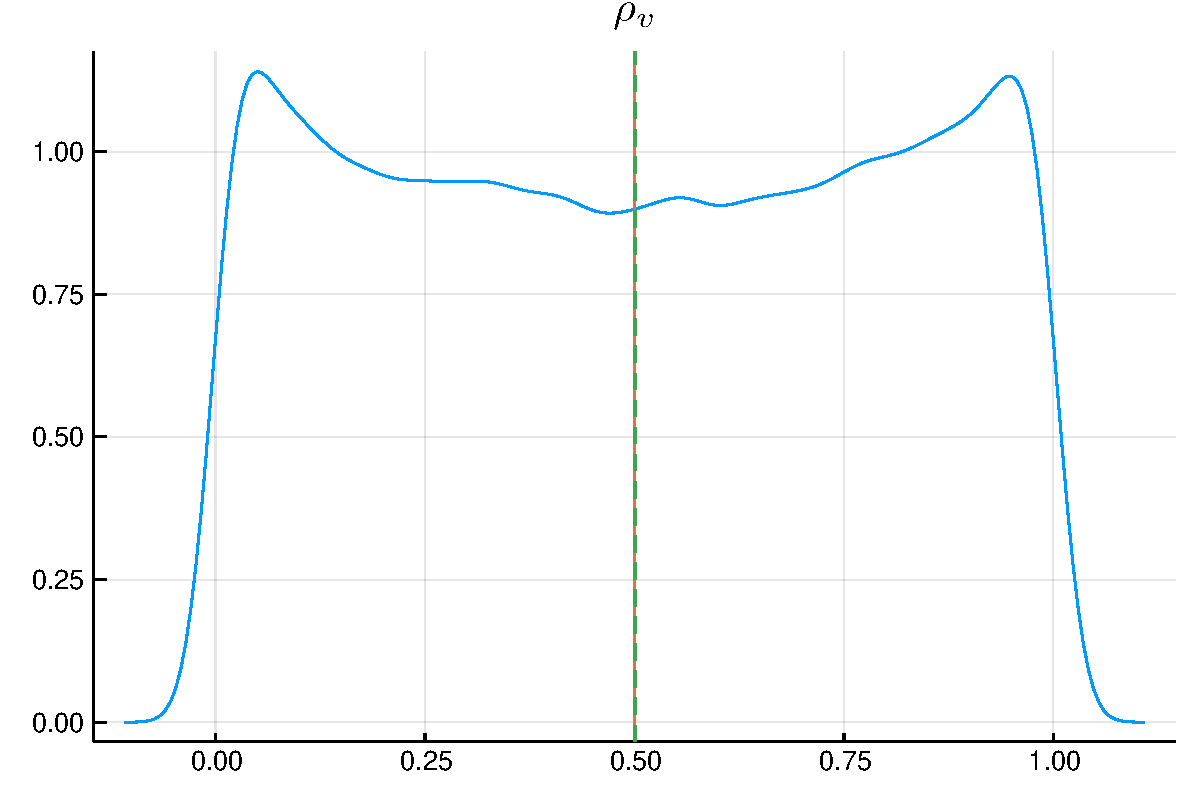
\includegraphics[width=\linewidth]{figures/dsge_and_julia_43_1.pdf}

The results are mostly positive, with means always close to the true value of the parameters. The distribution of $\rho_v$ is problematic, being a lot more disperse then their RWMH counterpart. We conduct more comparisons in what follows.

\subsubsection{Comparing HMC and RWMH}
Two things are important: precision and speed. We plot the distribution of the parameters from both the MCMC and the HMC to get an idea of their accuracy:


\begin{lstlisting}
(*@\HLJLn{pars{\_}hmc}@*) (*@\HLJLoB{=}@*) (*@\HLJLnf{load}@*)(*@\HLJLp{(}@*)(*@\HLJLs{"{}data/hmc2.jld"{}}@*)(*@\HLJLp{)[}@*)(*@\HLJLs{"{}pars"{}}@*)(*@\HLJLp{]}@*)

(*@\HLJLn{StatsPlots}@*)(*@\HLJLoB{.}@*)(*@\HLJLnf{density}@*)(*@\HLJLp{(}@*)(*@\HLJLn{pars{\_}hmc}@*)(*@\HLJLp{[}@*)(*@\HLJLoB{:}@*)(*@\HLJLp{,}@*)(*@\HLJLni{1}@*)(*@\HLJLp{],}@*) (*@\HLJLn{label}@*) (*@\HLJLoB{=}@*) (*@\HLJLs{"{}HMC"{}}@*)(*@\HLJLp{)}@*)
(*@\HLJLn{StatsPlots}@*)(*@\HLJLoB{.}@*)(*@\HLJLnf{density!}@*)(*@\HLJLp{(}@*)(*@\HLJLn{pars{\_}convertidos}@*)(*@\HLJLp{[}@*)(*@\HLJLni{50001}@*)(*@\HLJLoB{:}@*)(*@\HLJLni{100000}@*)(*@\HLJLp{,}@*)(*@\HLJLni{1}@*)(*@\HLJLp{],}@*) (*@\HLJLn{label}@*) (*@\HLJLoB{=}@*) (*@\HLJLs{"{}RWMH"{}}@*)(*@\HLJLp{)}@*)
(*@\HLJLnf{title!}@*)(*@\HLJLp{(}@*)(*@\HLJLso{L"{}{\textbackslash}beta"{}}@*)(*@\HLJLp{)}@*)
(*@\HLJLnf{vline!}@*)(*@\HLJLp{([}@*)(*@\HLJLn{true{\_}pars}@*)(*@\HLJLp{[}@*)(*@\HLJLsc{:bet}@*)(*@\HLJLp{]],}@*) (*@\HLJLn{label}@*) (*@\HLJLoB{=}@*) (*@\HLJLs{"{}True}@*) (*@\HLJLs{value"{}}@*)(*@\HLJLp{)}@*)
\end{lstlisting}

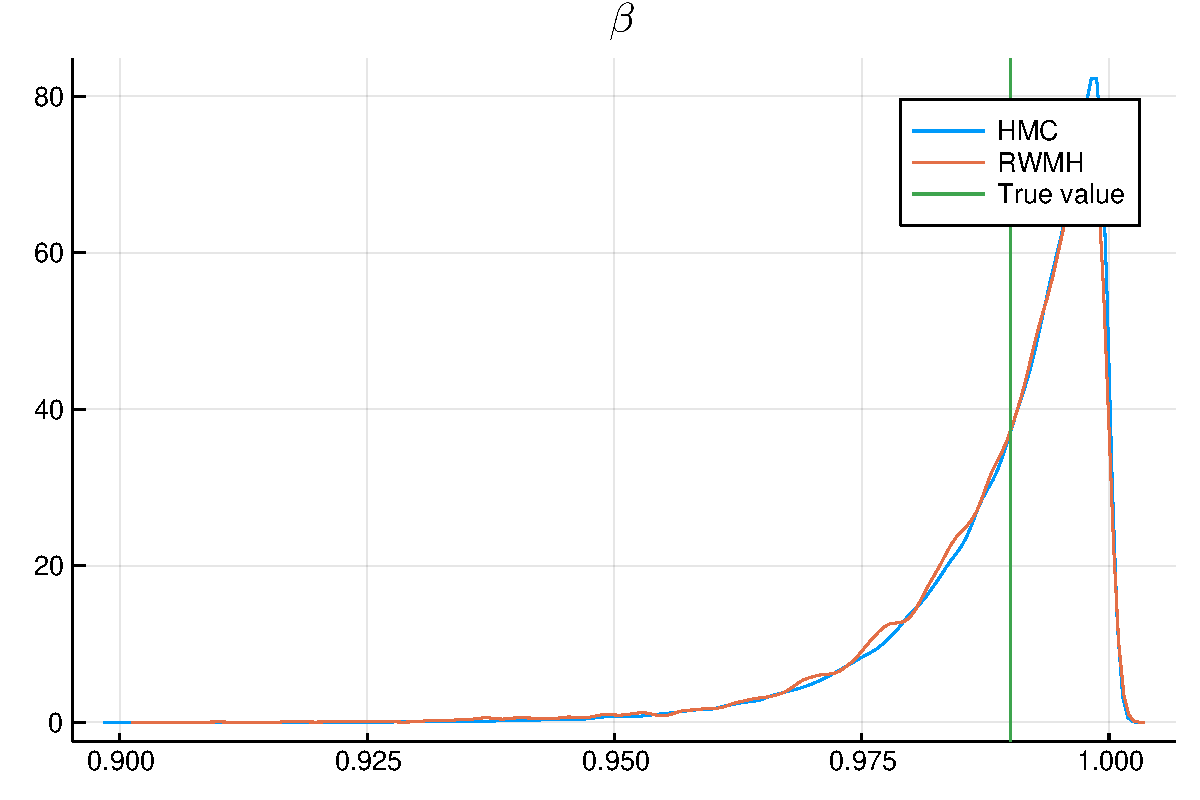
\includegraphics[width=\linewidth]{figures/dsge_and_julia_44_1.pdf}

\begin{lstlisting}
(*@\HLJLn{StatsPlots}@*)(*@\HLJLoB{.}@*)(*@\HLJLnf{density}@*)(*@\HLJLp{(}@*)(*@\HLJLn{pars{\_}hmc}@*)(*@\HLJLp{[}@*)(*@\HLJLoB{:}@*)(*@\HLJLp{,}@*)(*@\HLJLni{2}@*)(*@\HLJLp{],}@*) (*@\HLJLn{label}@*) (*@\HLJLoB{=}@*) (*@\HLJLs{"{}HMC"{}}@*)(*@\HLJLp{)}@*)
(*@\HLJLn{StatsPlots}@*)(*@\HLJLoB{.}@*)(*@\HLJLnf{density!}@*)(*@\HLJLp{(}@*)(*@\HLJLn{pars{\_}convertidos}@*)(*@\HLJLp{[}@*)(*@\HLJLni{50001}@*)(*@\HLJLoB{:}@*)(*@\HLJLni{100000}@*)(*@\HLJLp{,}@*)(*@\HLJLni{2}@*)(*@\HLJLp{],}@*) (*@\HLJLn{label}@*) (*@\HLJLoB{=}@*) (*@\HLJLs{"{}RWMH"{}}@*)(*@\HLJLp{)}@*)
(*@\HLJLnf{title!}@*)(*@\HLJLp{(}@*)(*@\HLJLso{L"{}{\textbackslash}epsilon"{}}@*)(*@\HLJLp{)}@*)
(*@\HLJLnf{vline!}@*)(*@\HLJLp{([}@*)(*@\HLJLn{true{\_}pars}@*)(*@\HLJLp{[}@*)(*@\HLJLsc{:epsilon}@*)(*@\HLJLp{]],}@*) (*@\HLJLn{label}@*) (*@\HLJLoB{=}@*) (*@\HLJLs{"{}True}@*) (*@\HLJLs{value"{}}@*)(*@\HLJLp{)}@*)
\end{lstlisting}

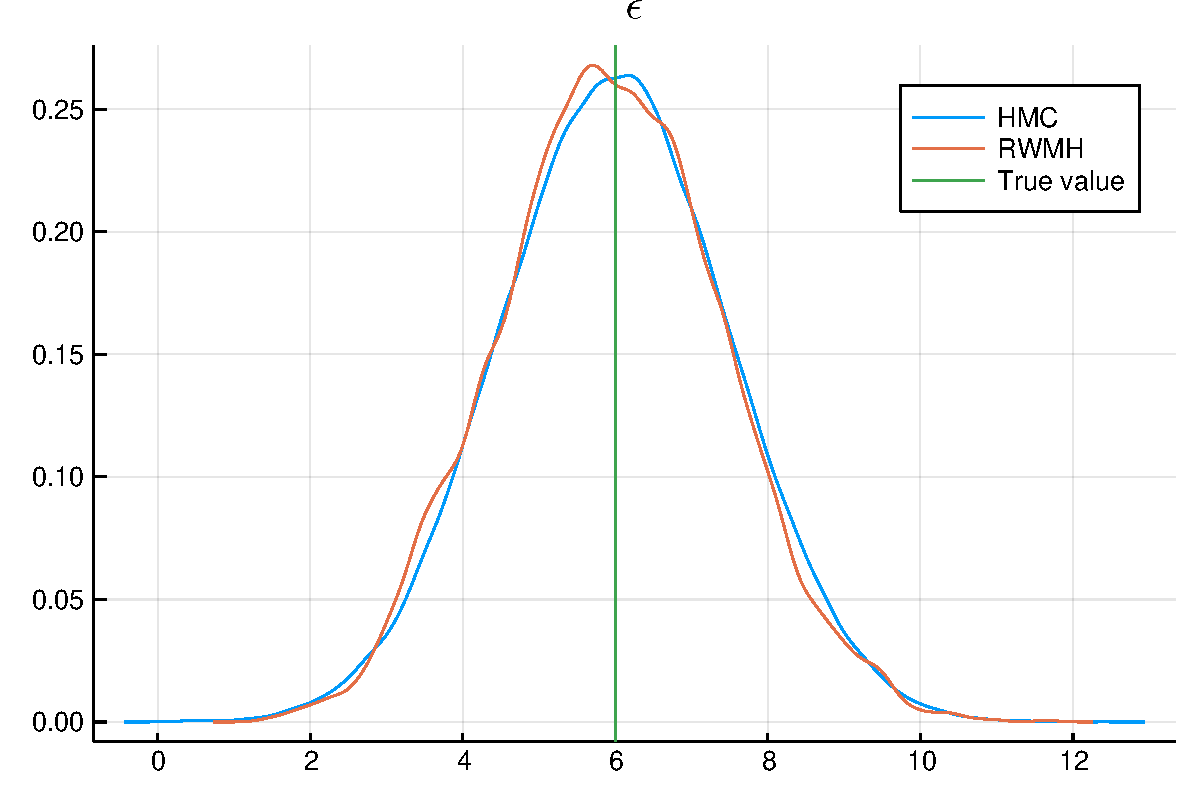
\includegraphics[width=\linewidth]{figures/dsge_and_julia_45_1.pdf}

\begin{lstlisting}
(*@\HLJLn{StatsPlots}@*)(*@\HLJLoB{.}@*)(*@\HLJLnf{density}@*)(*@\HLJLp{(}@*)(*@\HLJLn{pars{\_}hmc}@*)(*@\HLJLp{[}@*)(*@\HLJLoB{:}@*)(*@\HLJLp{,}@*)(*@\HLJLni{3}@*)(*@\HLJLp{],}@*) (*@\HLJLn{label}@*) (*@\HLJLoB{=}@*) (*@\HLJLs{"{}HMC"{}}@*)(*@\HLJLp{)}@*)
(*@\HLJLn{StatsPlots}@*)(*@\HLJLoB{.}@*)(*@\HLJLnf{density!}@*)(*@\HLJLp{(}@*)(*@\HLJLn{pars{\_}convertidos}@*)(*@\HLJLp{[}@*)(*@\HLJLni{50001}@*)(*@\HLJLoB{:}@*)(*@\HLJLni{100000}@*)(*@\HLJLp{,}@*)(*@\HLJLni{3}@*)(*@\HLJLp{],}@*) (*@\HLJLn{label}@*) (*@\HLJLoB{=}@*) (*@\HLJLs{"{}RWMH"{}}@*)(*@\HLJLp{)}@*)
(*@\HLJLnf{title!}@*)(*@\HLJLp{(}@*)(*@\HLJLso{L"{}{\textbackslash}theta"{}}@*)(*@\HLJLp{)}@*)
(*@\HLJLnf{vline!}@*)(*@\HLJLp{([}@*)(*@\HLJLn{true{\_}pars}@*)(*@\HLJLp{[}@*)(*@\HLJLsc{:theta}@*)(*@\HLJLp{]],}@*) (*@\HLJLn{label}@*) (*@\HLJLoB{=}@*) (*@\HLJLs{"{}True}@*) (*@\HLJLs{value"{}}@*)(*@\HLJLp{)}@*)
\end{lstlisting}

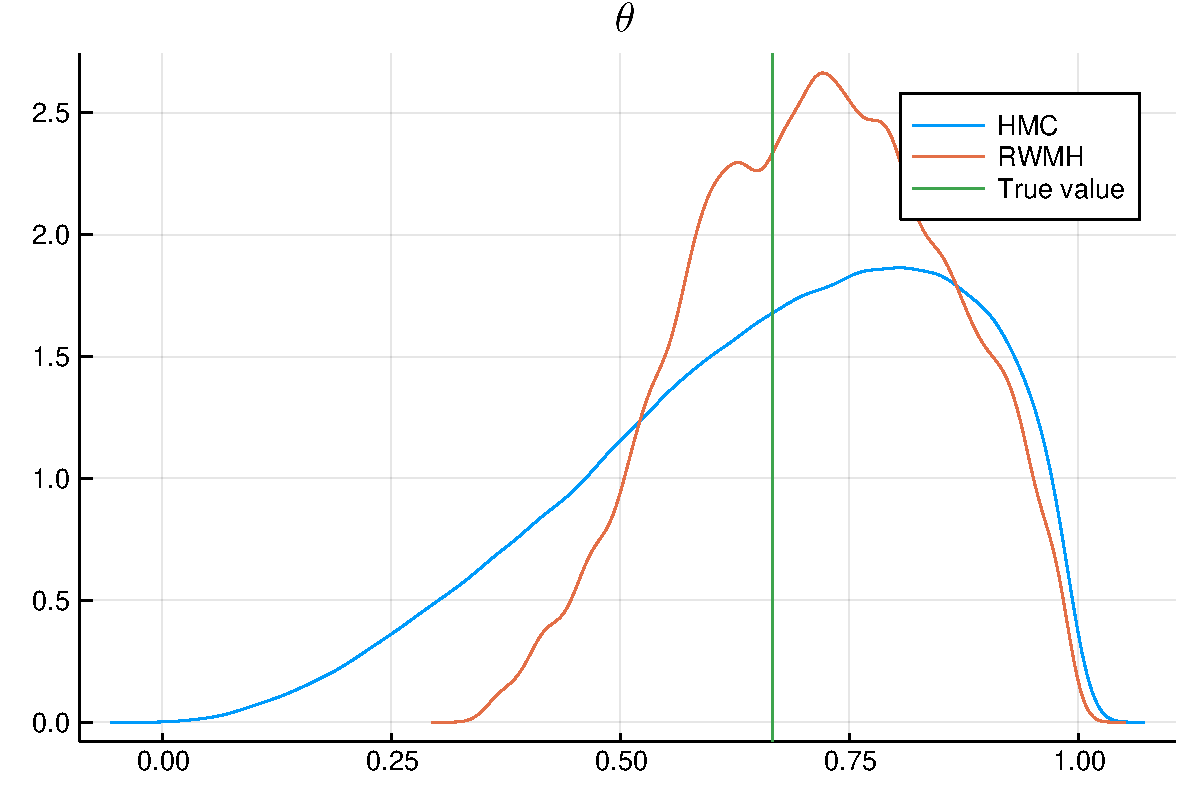
\includegraphics[width=\linewidth]{figures/dsge_and_julia_46_1.pdf}

\begin{lstlisting}
(*@\HLJLn{StatsPlots}@*)(*@\HLJLoB{.}@*)(*@\HLJLnf{density}@*)(*@\HLJLp{(}@*)(*@\HLJLn{pars{\_}hmc}@*)(*@\HLJLp{[}@*)(*@\HLJLoB{:}@*)(*@\HLJLp{,}@*)(*@\HLJLni{4}@*)(*@\HLJLp{],}@*) (*@\HLJLn{label}@*) (*@\HLJLoB{=}@*) (*@\HLJLs{"{}HMC"{}}@*)(*@\HLJLp{)}@*)
(*@\HLJLn{StatsPlots}@*)(*@\HLJLoB{.}@*)(*@\HLJLnf{density!}@*)(*@\HLJLp{(}@*)(*@\HLJLn{pars{\_}convertidos}@*)(*@\HLJLp{[}@*)(*@\HLJLni{50001}@*)(*@\HLJLoB{:}@*)(*@\HLJLni{100000}@*)(*@\HLJLp{,}@*)(*@\HLJLni{4}@*)(*@\HLJLp{],}@*) (*@\HLJLn{label}@*) (*@\HLJLoB{=}@*) (*@\HLJLs{"{}RWMH"{}}@*)(*@\HLJLp{)}@*)
(*@\HLJLnf{title!}@*)(*@\HLJLp{(}@*)(*@\HLJLso{L"{}{\textbackslash}sigma"{}}@*)(*@\HLJLp{)}@*)
(*@\HLJLnf{vline!}@*)(*@\HLJLp{([}@*)(*@\HLJLn{true{\_}pars}@*)(*@\HLJLp{[}@*)(*@\HLJLsc{:sig}@*)(*@\HLJLp{]],}@*) (*@\HLJLn{label}@*) (*@\HLJLoB{=}@*) (*@\HLJLs{"{}True}@*) (*@\HLJLs{value"{}}@*)(*@\HLJLp{)}@*)
\end{lstlisting}

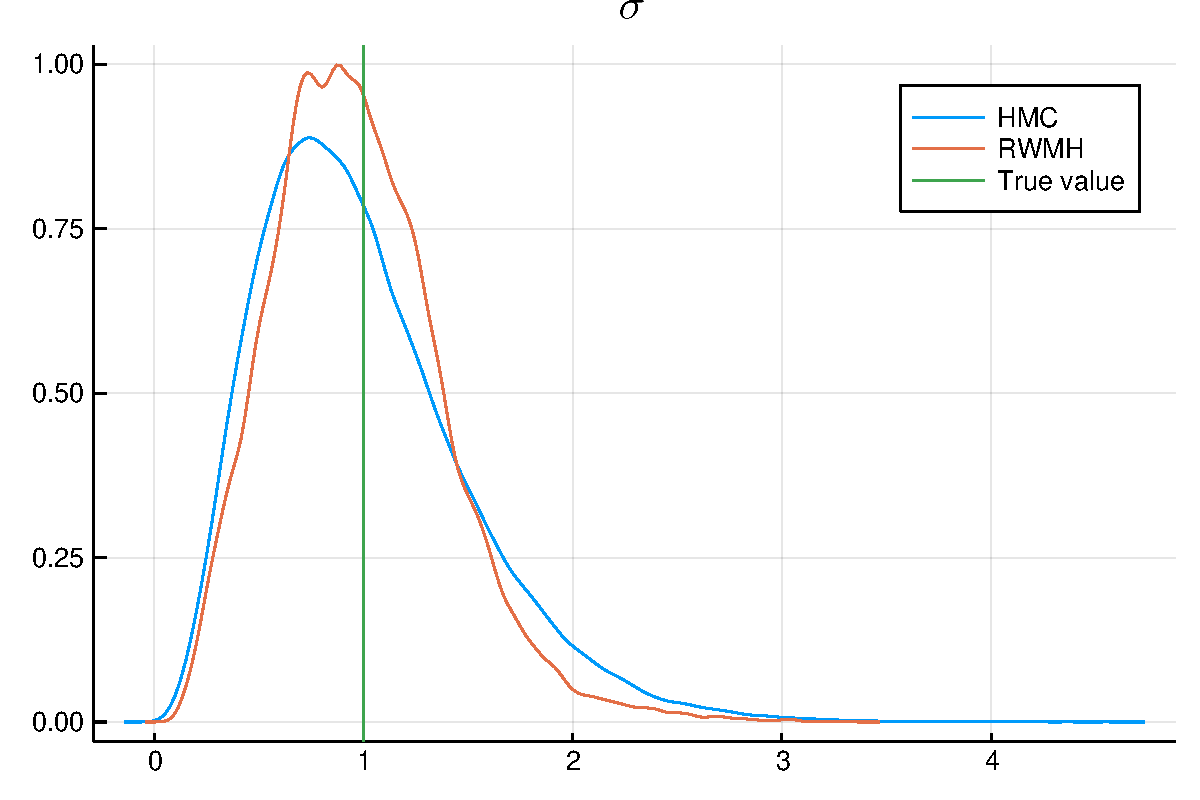
\includegraphics[width=\linewidth]{figures/dsge_and_julia_47_1.pdf}

\begin{lstlisting}
(*@\HLJLn{StatsPlots}@*)(*@\HLJLoB{.}@*)(*@\HLJLnf{density}@*)(*@\HLJLp{(}@*)(*@\HLJLn{pars{\_}hmc}@*)(*@\HLJLp{[}@*)(*@\HLJLoB{:}@*)(*@\HLJLp{,}@*)(*@\HLJLni{5}@*)(*@\HLJLp{],}@*) (*@\HLJLn{label}@*) (*@\HLJLoB{=}@*) (*@\HLJLs{"{}HMC"{}}@*)(*@\HLJLp{)}@*)
(*@\HLJLn{StatsPlots}@*)(*@\HLJLoB{.}@*)(*@\HLJLnf{density!}@*)(*@\HLJLp{(}@*)(*@\HLJLn{pars{\_}convertidos}@*)(*@\HLJLp{[}@*)(*@\HLJLni{50001}@*)(*@\HLJLoB{:}@*)(*@\HLJLni{100000}@*)(*@\HLJLp{,}@*)(*@\HLJLni{5}@*)(*@\HLJLp{],}@*) (*@\HLJLn{label}@*) (*@\HLJLoB{=}@*) (*@\HLJLs{"{}RWMH"{}}@*)(*@\HLJLp{)}@*)
(*@\HLJLnf{title!}@*)(*@\HLJLp{(}@*)(*@\HLJLso{L"{}{\textbackslash}sigma{\textasciicircum}2"{}}@*)(*@\HLJLp{)}@*)
(*@\HLJLnf{vline!}@*)(*@\HLJLp{([}@*)(*@\HLJLn{true{\_}pars}@*)(*@\HLJLp{[}@*)(*@\HLJLsc{:s2}@*)(*@\HLJLp{]],}@*) (*@\HLJLn{label}@*) (*@\HLJLoB{=}@*) (*@\HLJLs{"{}True}@*) (*@\HLJLs{value"{}}@*)(*@\HLJLp{)}@*)
\end{lstlisting}

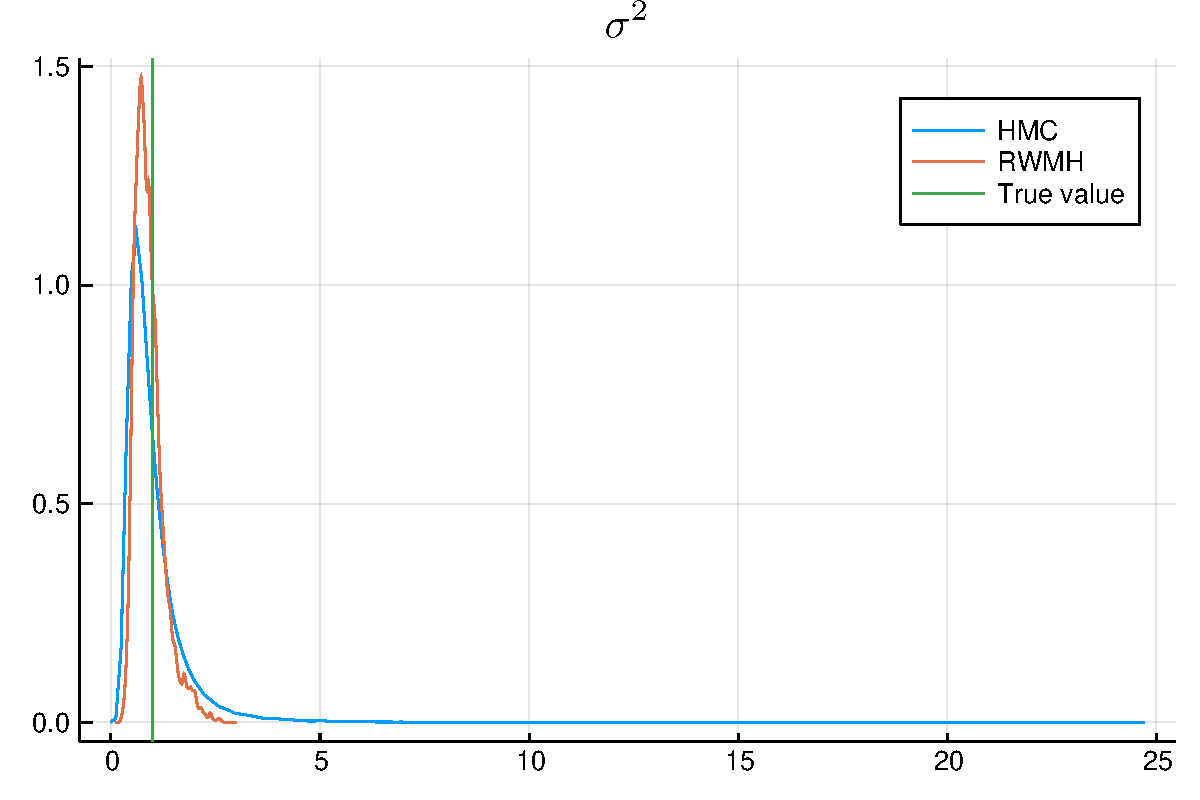
\includegraphics[width=\linewidth]{figures/dsge_and_julia_48_1.pdf}

\begin{lstlisting}
(*@\HLJLn{StatsPlots}@*)(*@\HLJLoB{.}@*)(*@\HLJLnf{density}@*)(*@\HLJLp{(}@*)(*@\HLJLn{pars{\_}hmc}@*)(*@\HLJLp{[}@*)(*@\HLJLoB{:}@*)(*@\HLJLp{,}@*)(*@\HLJLni{6}@*)(*@\HLJLp{],}@*) (*@\HLJLn{label}@*) (*@\HLJLoB{=}@*) (*@\HLJLs{"{}HMC"{}}@*)(*@\HLJLp{)}@*)
(*@\HLJLn{StatsPlots}@*)(*@\HLJLoB{.}@*)(*@\HLJLnf{density!}@*)(*@\HLJLp{(}@*)(*@\HLJLn{pars{\_}convertidos}@*)(*@\HLJLp{[}@*)(*@\HLJLni{50001}@*)(*@\HLJLoB{:}@*)(*@\HLJLni{100000}@*)(*@\HLJLp{,}@*)(*@\HLJLni{6}@*)(*@\HLJLp{],}@*) (*@\HLJLn{label}@*) (*@\HLJLoB{=}@*) (*@\HLJLs{"{}RWMH"{}}@*)(*@\HLJLp{)}@*)
(*@\HLJLnf{title!}@*)(*@\HLJLp{(}@*)(*@\HLJLso{L"{}{\textbackslash}phi"{}}@*)(*@\HLJLp{)}@*)
(*@\HLJLnf{vline!}@*)(*@\HLJLp{([}@*)(*@\HLJLn{true{\_}pars}@*)(*@\HLJLp{[}@*)(*@\HLJLsc{:phi}@*)(*@\HLJLp{]],}@*) (*@\HLJLn{label}@*) (*@\HLJLoB{=}@*) (*@\HLJLs{"{}True}@*) (*@\HLJLs{value"{}}@*)(*@\HLJLp{)}@*)
\end{lstlisting}

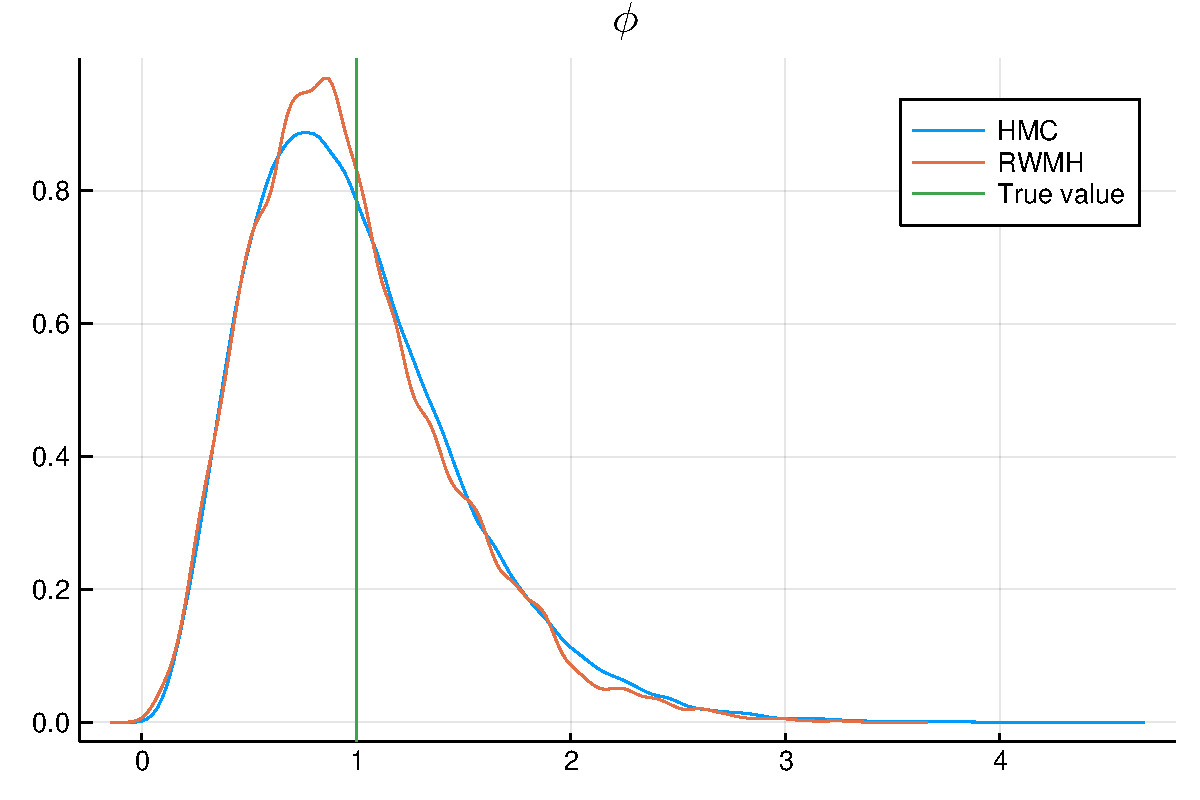
\includegraphics[width=\linewidth]{figures/dsge_and_julia_49_1.pdf}

\begin{lstlisting}
(*@\HLJLn{StatsPlots}@*)(*@\HLJLoB{.}@*)(*@\HLJLnf{density}@*)(*@\HLJLp{(}@*)(*@\HLJLn{pars{\_}hmc}@*)(*@\HLJLp{[}@*)(*@\HLJLoB{:}@*)(*@\HLJLp{,}@*)(*@\HLJLni{7}@*)(*@\HLJLp{],}@*) (*@\HLJLn{label}@*) (*@\HLJLoB{=}@*) (*@\HLJLs{"{}HMC"{}}@*)(*@\HLJLp{)}@*)
(*@\HLJLn{StatsPlots}@*)(*@\HLJLoB{.}@*)(*@\HLJLnf{density!}@*)(*@\HLJLp{(}@*)(*@\HLJLn{pars{\_}convertidos}@*)(*@\HLJLp{[}@*)(*@\HLJLni{50001}@*)(*@\HLJLoB{:}@*)(*@\HLJLni{100000}@*)(*@\HLJLp{,}@*)(*@\HLJLni{7}@*)(*@\HLJLp{],}@*) (*@\HLJLn{label}@*) (*@\HLJLoB{=}@*) (*@\HLJLs{"{}RWMH"{}}@*)(*@\HLJLp{)}@*)
(*@\HLJLnf{title!}@*)(*@\HLJLp{(}@*)(*@\HLJLso{L"{}{\textbackslash}phi{\_}{\{}{\textbackslash}pi{\}}"{}}@*)(*@\HLJLp{)}@*)
(*@\HLJLnf{vline!}@*)(*@\HLJLp{([}@*)(*@\HLJLn{true{\_}pars}@*)(*@\HLJLp{[}@*)(*@\HLJLsc{:phi{\_}pi}@*)(*@\HLJLp{]],}@*) (*@\HLJLn{label}@*) (*@\HLJLoB{=}@*) (*@\HLJLs{"{}True}@*) (*@\HLJLs{value"{}}@*)(*@\HLJLp{)}@*)
\end{lstlisting}

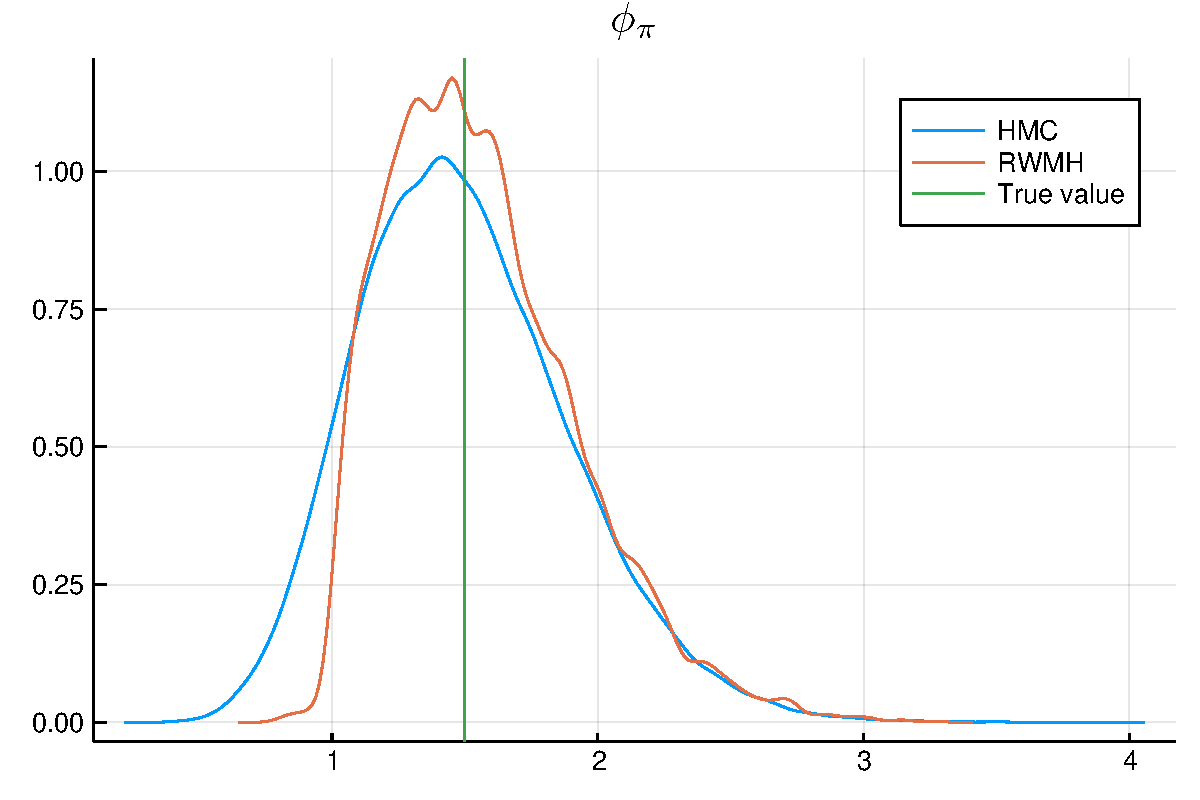
\includegraphics[width=\linewidth]{figures/dsge_and_julia_50_1.pdf}

\begin{lstlisting}
(*@\HLJLn{StatsPlots}@*)(*@\HLJLoB{.}@*)(*@\HLJLnf{density}@*)(*@\HLJLp{(}@*)(*@\HLJLn{pars{\_}hmc}@*)(*@\HLJLp{[}@*)(*@\HLJLoB{:}@*)(*@\HLJLp{,}@*)(*@\HLJLni{8}@*)(*@\HLJLp{],}@*) (*@\HLJLn{label}@*) (*@\HLJLoB{=}@*) (*@\HLJLs{"{}HMC"{}}@*)(*@\HLJLp{)}@*)
(*@\HLJLn{StatsPlots}@*)(*@\HLJLoB{.}@*)(*@\HLJLnf{density!}@*)(*@\HLJLp{(}@*)(*@\HLJLn{pars{\_}convertidos}@*)(*@\HLJLp{[}@*)(*@\HLJLni{50001}@*)(*@\HLJLoB{:}@*)(*@\HLJLni{100000}@*)(*@\HLJLp{,}@*)(*@\HLJLni{8}@*)(*@\HLJLp{],}@*) (*@\HLJLn{label}@*) (*@\HLJLoB{=}@*) (*@\HLJLs{"{}RWMH"{}}@*)(*@\HLJLp{)}@*)
(*@\HLJLnf{title!}@*)(*@\HLJLp{(}@*)(*@\HLJLso{L"{}{\textbackslash}phi{\_}y"{}}@*)(*@\HLJLp{)}@*)
(*@\HLJLnf{vline!}@*)(*@\HLJLp{([}@*)(*@\HLJLn{true{\_}pars}@*)(*@\HLJLp{[}@*)(*@\HLJLsc{:phi{\_}y}@*)(*@\HLJLp{]],}@*) (*@\HLJLn{label}@*) (*@\HLJLoB{=}@*) (*@\HLJLs{"{}True}@*) (*@\HLJLs{value"{}}@*)(*@\HLJLp{)}@*)
\end{lstlisting}

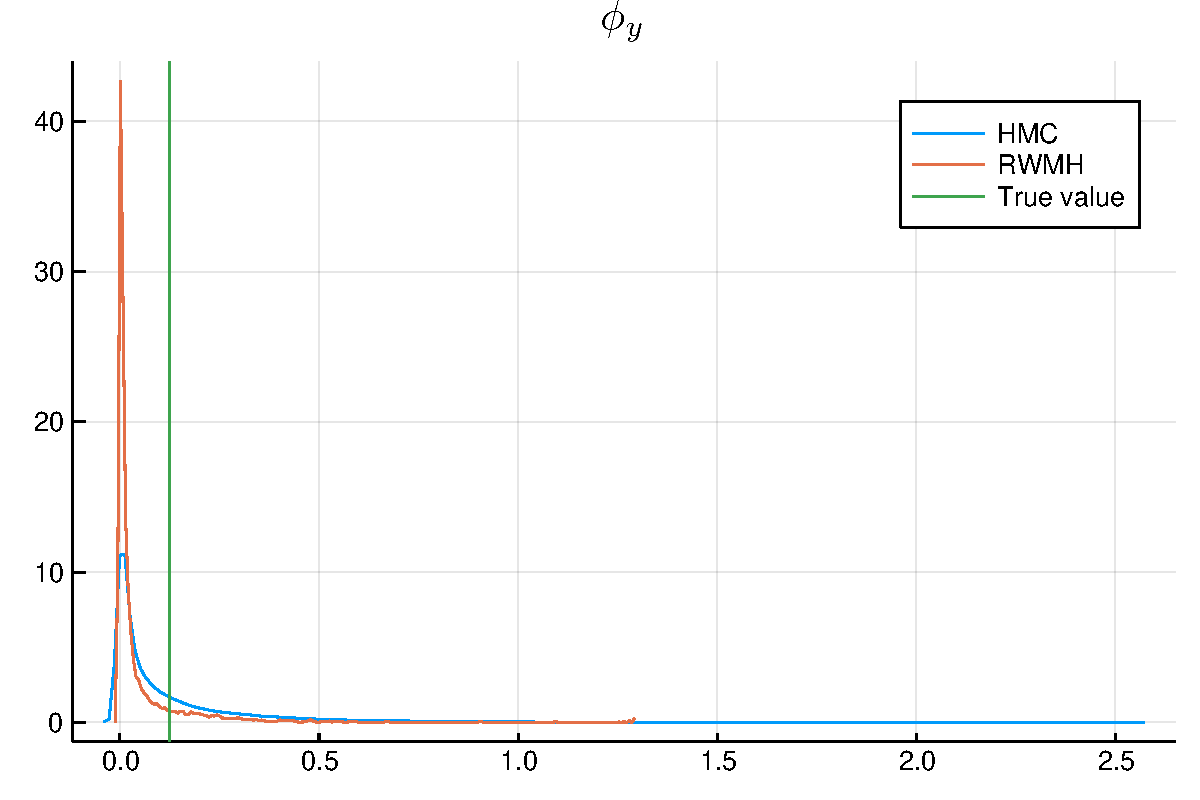
\includegraphics[width=\linewidth]{figures/dsge_and_julia_51_1.pdf}

\begin{lstlisting}
(*@\HLJLn{StatsPlots}@*)(*@\HLJLoB{.}@*)(*@\HLJLnf{density}@*)(*@\HLJLp{(}@*)(*@\HLJLn{pars{\_}hmc}@*)(*@\HLJLp{[}@*)(*@\HLJLoB{:}@*)(*@\HLJLp{,}@*)(*@\HLJLni{9}@*)(*@\HLJLp{],}@*) (*@\HLJLn{label}@*) (*@\HLJLoB{=}@*) (*@\HLJLs{"{}HMC"{}}@*)(*@\HLJLp{)}@*)
(*@\HLJLn{StatsPlots}@*)(*@\HLJLoB{.}@*)(*@\HLJLnf{density!}@*)(*@\HLJLp{(}@*)(*@\HLJLn{pars{\_}convertidos}@*)(*@\HLJLp{[}@*)(*@\HLJLni{50001}@*)(*@\HLJLoB{:}@*)(*@\HLJLni{100000}@*)(*@\HLJLp{,}@*)(*@\HLJLni{9}@*)(*@\HLJLp{],}@*) (*@\HLJLn{label}@*) (*@\HLJLoB{=}@*) (*@\HLJLs{"{}RWMH"{}}@*)(*@\HLJLp{)}@*)
(*@\HLJLnf{title!}@*)(*@\HLJLp{(}@*)(*@\HLJLso{L"{}{\textbackslash}rho{\_}v"{}}@*)(*@\HLJLp{)}@*)
(*@\HLJLnf{vline!}@*)(*@\HLJLp{([}@*)(*@\HLJLn{true{\_}pars}@*)(*@\HLJLp{[}@*)(*@\HLJLsc{:rho{\_}v}@*)(*@\HLJLp{]],}@*) (*@\HLJLn{label}@*) (*@\HLJLoB{=}@*) (*@\HLJLs{"{}True}@*) (*@\HLJLs{value"{}}@*)(*@\HLJLp{)}@*)
\end{lstlisting}

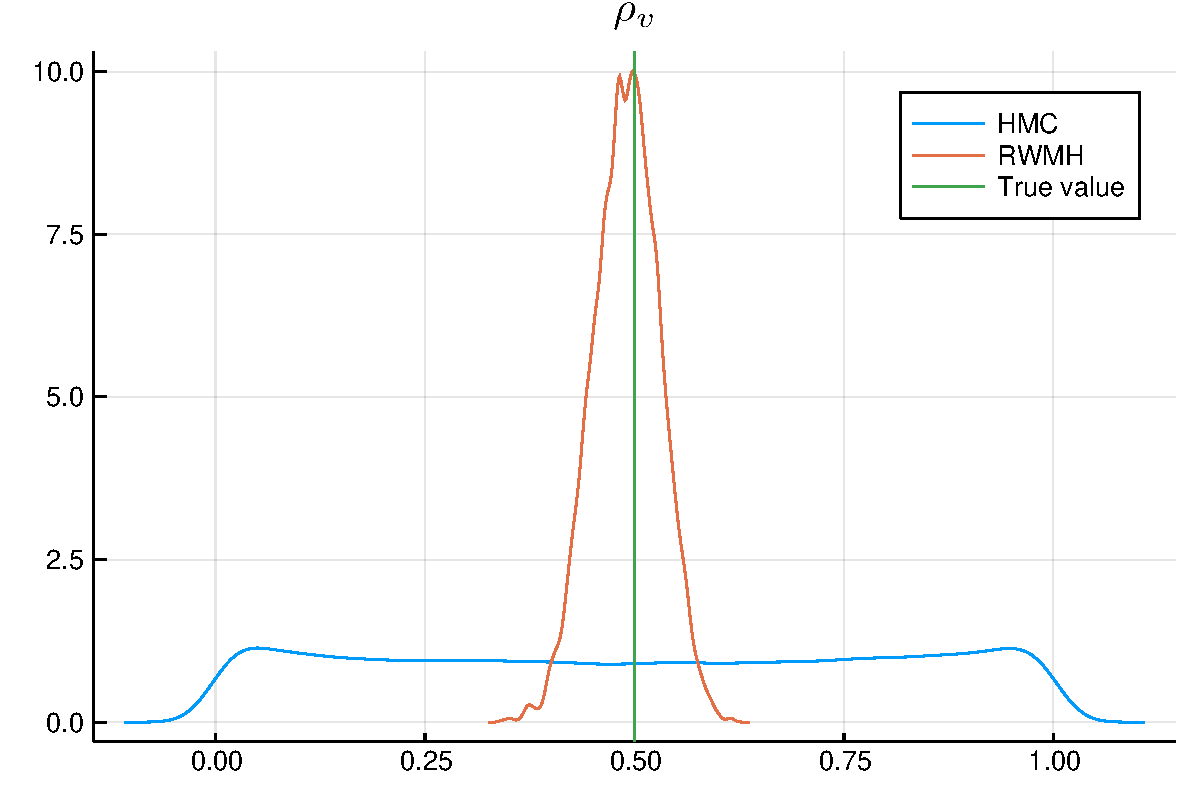
\includegraphics[width=\linewidth]{figures/dsge_and_julia_52_1.pdf}

On the time front, we will do two sets of simulations: one with 10 thousand replications and another with 100 thousand. We would expect that the time difference would be around 10 times, and it is in the ballpark. While we let the HMC procedure choose the optimal parameter, and therefore the time before the actually iteration begins enters in our time figure, we feed the optimal parameter to the MCMC without taking this time into account in the table bellow. The time takes into account the warm up in both case. We conduct this simulations in a Dell Vostro with an Intel dual core i5-3210 at 2.5 Ghz, and with 6 GB of ram. The OS is a Linux flavour. Since we are more interested in the relative performance, this facts are by themselves of little importance. The times are, in seconds:

\begin{table}[h]
	\centering
	\caption{Time, in seconds, for estimating the models using RWMH and HMC}	
	\begin{tabular}{r | r | r}
		Replications & RWMH & HMC \\
		\hline
		10,000 & 252 & 46 \\
		100,000 & 2632 & 400 \\
	\end{tabular}
\end{table}

Hamiltonian Monte carlo is not just faster: it is \emph{a lot faster}. This hides fundamental differences between the two methods: the number of iterations necessary to obtain convergence. To illustrate this point, we show the results of only ten thousand iterations of each algorithm:

\begin{lstlisting}
(*@\HLJLn{pars{\_}aceitos}@*) (*@\HLJLoB{=}@*) (*@\HLJLnf{load}@*)(*@\HLJLp{(}@*)(*@\HLJLs{"{}data/mcmc10k.jld"{}}@*)(*@\HLJLp{)[}@*)(*@\HLJLs{"{}pars"{}}@*)(*@\HLJLp{]}@*)

(*@\HLJLn{yy}@*)(*@\HLJLp{,}@*)(*@\HLJLn{shocks}@*) (*@\HLJLoB{=}@*) (*@\HLJLnf{simulate{\_}dsge}@*)(*@\HLJLp{(}@*)(*@\HLJLn{GAMMA{\_}0}@*)(*@\HLJLp{,}@*)(*@\HLJLn{GAMMA{\_}1}@*)(*@\HLJLp{,}@*)(*@\HLJLn{PSI}@*)(*@\HLJLp{,}@*)(*@\HLJLn{PI}@*)(*@\HLJLp{,}@*)(*@\HLJLni{500}@*)(*@\HLJLp{)}@*)

(*@\HLJLn{pars{\_}convertidos10k}@*) (*@\HLJLoB{=}@*) (*@\HLJLnf{zeros}@*)(*@\HLJLp{(}@*)(*@\HLJLni{10000}@*)(*@\HLJLp{,}@*)(*@\HLJLni{9}@*)(*@\HLJLp{)}@*)

(*@\HLJLk{for}@*) (*@\HLJLn{i}@*) (*@\HLJLkp{in}@*) (*@\HLJLni{1}@*)(*@\HLJLoB{:}@*)(*@\HLJLni{10000}@*)
    (*@\HLJLnd{@unpack}@*) (*@\HLJLn{bet}@*)(*@\HLJLp{,}@*)(*@\HLJLn{epsilon}@*)(*@\HLJLp{,}@*)(*@\HLJLn{theta}@*)(*@\HLJLp{,}@*)(*@\HLJLn{sig}@*)(*@\HLJLp{,}@*)(*@\HLJLn{s2}@*)(*@\HLJLp{,}@*)(*@\HLJLn{phi}@*)(*@\HLJLp{,}@*)(*@\HLJLn{phi{\_}pi}@*)(*@\HLJLp{,}@*)(*@\HLJLn{phi{\_}y}@*)(*@\HLJLp{,}@*)(*@\HLJLn{rho{\_}v}@*) (*@\HLJLoB{=}@*) (*@\HLJLn{TransformVariables}@*)(*@\HLJLoB{.}@*)(*@\HLJLnf{transform}@*)(*@\HLJLp{(}@*)(*@\HLJLn{t}@*)(*@\HLJLp{,}@*)(*@\HLJLn{pars{\_}aceitos}@*)(*@\HLJLp{[}@*)(*@\HLJLn{i}@*)(*@\HLJLp{,}@*)(*@\HLJLni{2}@*)(*@\HLJLoB{:}@*)(*@\HLJLni{10}@*)(*@\HLJLp{])}@*)
    (*@\HLJLn{pars{\_}convertidos10k}@*)(*@\HLJLp{[}@*)(*@\HLJLn{i}@*)(*@\HLJLp{,}@*)(*@\HLJLoB{:}@*)(*@\HLJLp{]}@*) (*@\HLJLoB{=}@*) (*@\HLJLp{[}@*)(*@\HLJLn{bet}@*)(*@\HLJLp{,}@*)(*@\HLJLn{epsilon}@*)(*@\HLJLp{,}@*)(*@\HLJLn{theta}@*)(*@\HLJLp{,}@*)(*@\HLJLn{sig}@*)(*@\HLJLp{,}@*)(*@\HLJLn{s2}@*)(*@\HLJLp{,}@*)(*@\HLJLn{phi}@*)(*@\HLJLp{,}@*)(*@\HLJLn{phi{\_}pi}@*)(*@\HLJLp{,}@*)(*@\HLJLn{phi{\_}y}@*)(*@\HLJLp{,}@*)(*@\HLJLn{rho{\_}v}@*)(*@\HLJLp{]}@*)(*@\HLJLcs{{\#}(bet}@*) (*@\HLJLcs{=}@*) (*@\HLJLcs{pars{\_}aceitos[i,2],}@*) (*@\HLJLcs{epsilon}@*) (*@\HLJLcs{=}@*) (*@\HLJLcs{pars{\_}aceitos[i,3],}@*) (*@\HLJLcs{theta}@*) (*@\HLJLcs{=}@*) (*@\HLJLcs{pars{\_}aceitos[i,4],sig}@*) (*@\HLJLcs{=}@*) (*@\HLJLcs{pars{\_}aceitos[i,5],s2}@*) (*@\HLJLcs{=}@*) (*@\HLJLcs{pars{\_}aceitos[i,6],phi}@*) (*@\HLJLcs{=}@*) (*@\HLJLcs{pars{\_}aceitos[i,7],phi{\_}pi}@*) (*@\HLJLcs{=}@*) (*@\HLJLcs{pars{\_}aceitos[i,8],phi{\_}y}@*) (*@\HLJLcs{=}@*) (*@\HLJLcs{pars{\_}aceitos[i,9],rho{\_}v}@*) (*@\HLJLcs{=}@*) (*@\HLJLcs{pars{\_}aceitos[i,10]))}@*)
(*@\HLJLk{end}@*)

(*@\HLJLn{pars{\_}hmc10k}@*) (*@\HLJLoB{=}@*) (*@\HLJLnf{load}@*)(*@\HLJLp{(}@*)(*@\HLJLs{"{}data/hmc10k.jld"{}}@*)(*@\HLJLp{)[}@*)(*@\HLJLs{"{}pars"{}}@*)(*@\HLJLp{]}@*)

(*@\HLJLn{StatsPlots}@*)(*@\HLJLoB{.}@*)(*@\HLJLnf{density}@*)(*@\HLJLp{(}@*)(*@\HLJLn{pars{\_}hmc10k}@*)(*@\HLJLp{[}@*)(*@\HLJLoB{:}@*)(*@\HLJLp{,}@*)(*@\HLJLni{1}@*)(*@\HLJLp{],}@*) (*@\HLJLn{label}@*) (*@\HLJLoB{=}@*) (*@\HLJLs{"{}HMC"{}}@*)(*@\HLJLp{,}@*) (*@\HLJLn{legend}@*) (*@\HLJLoB{=}@*) (*@\HLJLsc{:topleft}@*)(*@\HLJLp{)}@*)
(*@\HLJLn{StatsPlots}@*)(*@\HLJLoB{.}@*)(*@\HLJLnf{density!}@*)(*@\HLJLp{(}@*)(*@\HLJLn{pars{\_}convertidos10k}@*)(*@\HLJLp{[}@*)(*@\HLJLni{1}@*)(*@\HLJLoB{:}@*)(*@\HLJLni{10000}@*)(*@\HLJLp{,}@*)(*@\HLJLni{1}@*)(*@\HLJLp{],}@*) (*@\HLJLn{label}@*) (*@\HLJLoB{=}@*) (*@\HLJLs{"{}RWMH"{}}@*)(*@\HLJLp{)}@*)
(*@\HLJLnf{title!}@*)(*@\HLJLp{(}@*)(*@\HLJLso{L"{}{\textbackslash}beta"{}}@*)(*@\HLJLp{)}@*)
(*@\HLJLnf{vline!}@*)(*@\HLJLp{([}@*)(*@\HLJLn{true{\_}pars}@*)(*@\HLJLp{[}@*)(*@\HLJLsc{:bet}@*)(*@\HLJLp{]],}@*) (*@\HLJLn{label}@*) (*@\HLJLoB{=}@*) (*@\HLJLs{"{}True}@*) (*@\HLJLs{value"{}}@*)(*@\HLJLp{)}@*)
\end{lstlisting}

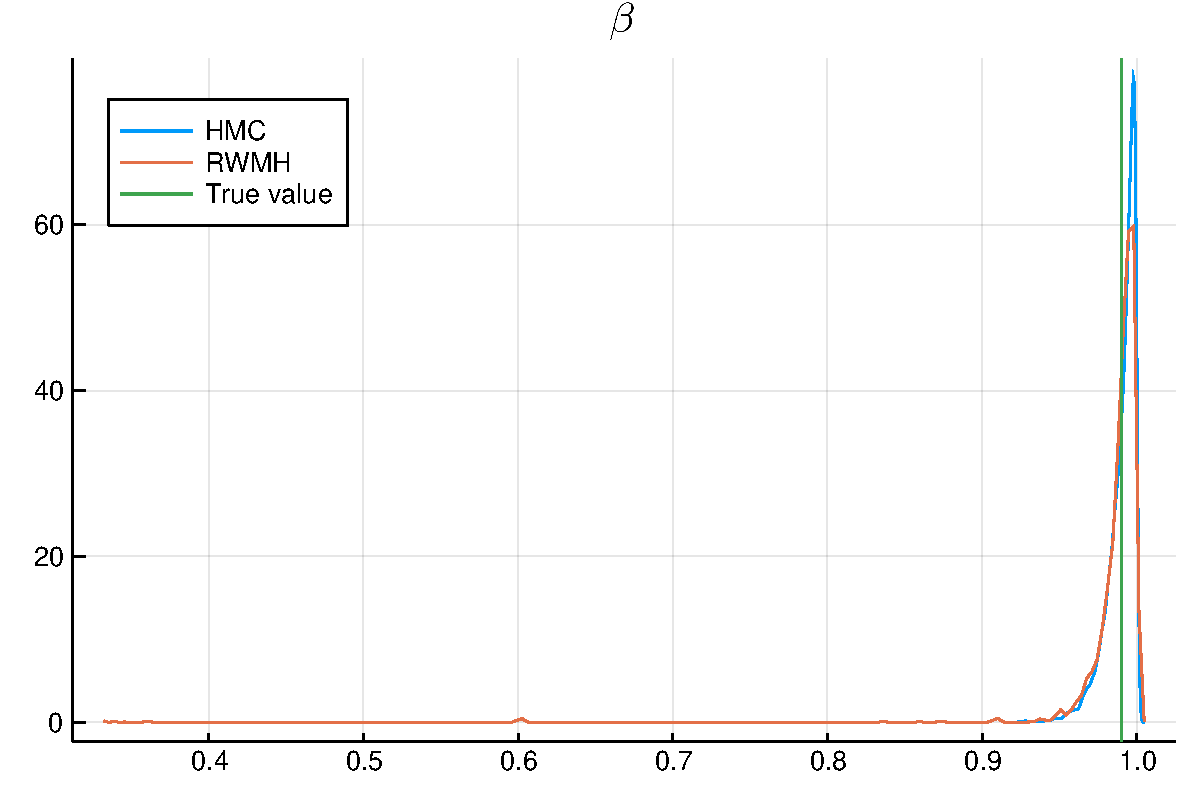
\includegraphics[width=\linewidth]{figures/dsge_and_julia_53_1.pdf}

\begin{lstlisting}
(*@\HLJLn{StatsPlots}@*)(*@\HLJLoB{.}@*)(*@\HLJLnf{density}@*)(*@\HLJLp{(}@*)(*@\HLJLn{pars{\_}hmc10k}@*)(*@\HLJLp{[}@*)(*@\HLJLoB{:}@*)(*@\HLJLp{,}@*)(*@\HLJLni{2}@*)(*@\HLJLp{],}@*) (*@\HLJLn{label}@*) (*@\HLJLoB{=}@*) (*@\HLJLs{"{}HMC"{}}@*)(*@\HLJLp{)}@*)
(*@\HLJLn{StatsPlots}@*)(*@\HLJLoB{.}@*)(*@\HLJLnf{density!}@*)(*@\HLJLp{(}@*)(*@\HLJLn{pars{\_}convertidos10k}@*)(*@\HLJLp{[}@*)(*@\HLJLni{1}@*)(*@\HLJLoB{:}@*)(*@\HLJLni{10000}@*)(*@\HLJLp{,}@*)(*@\HLJLni{2}@*)(*@\HLJLp{],}@*) (*@\HLJLn{label}@*) (*@\HLJLoB{=}@*) (*@\HLJLs{"{}RWMH"{}}@*)(*@\HLJLp{)}@*)
(*@\HLJLnf{title!}@*)(*@\HLJLp{(}@*)(*@\HLJLso{L"{}{\textbackslash}epsilon"{}}@*)(*@\HLJLp{)}@*)
(*@\HLJLnf{vline!}@*)(*@\HLJLp{([}@*)(*@\HLJLn{true{\_}pars}@*)(*@\HLJLp{[}@*)(*@\HLJLsc{:epsilon}@*)(*@\HLJLp{]],}@*) (*@\HLJLn{label}@*) (*@\HLJLoB{=}@*) (*@\HLJLs{"{}True}@*) (*@\HLJLs{value"{}}@*)(*@\HLJLp{)}@*)
\end{lstlisting}

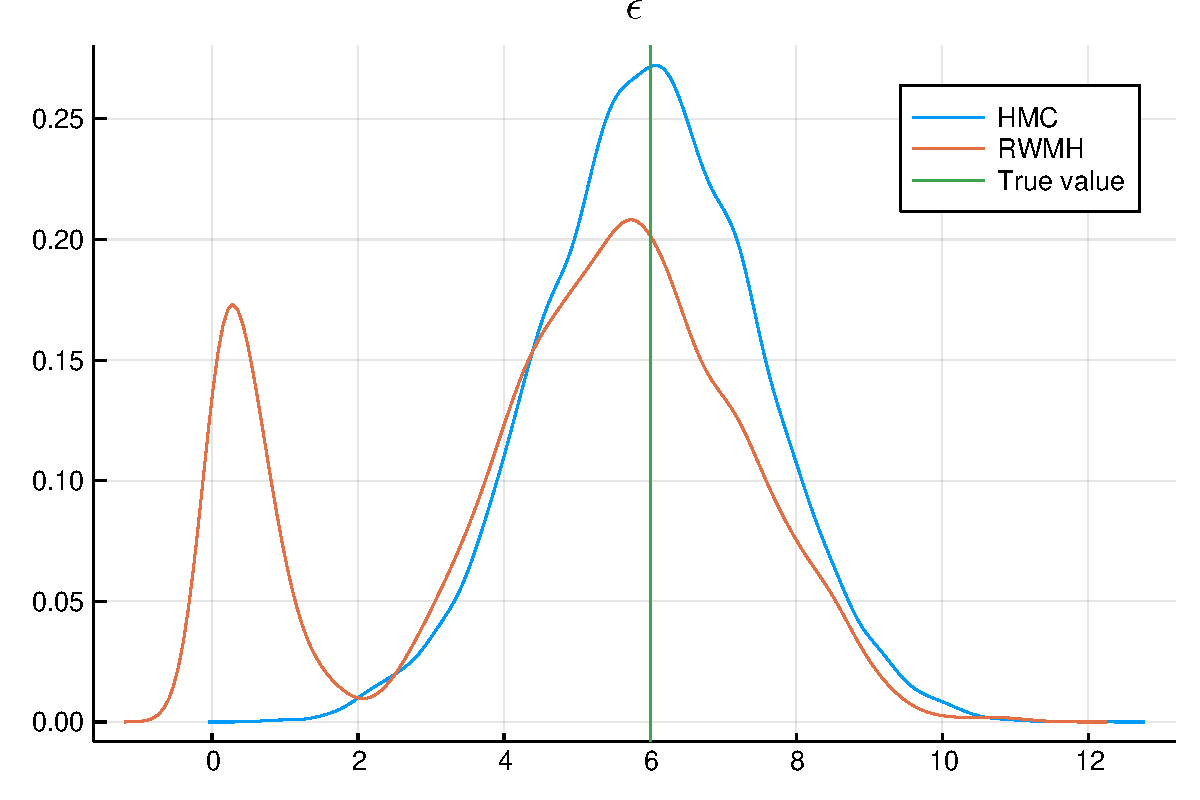
\includegraphics[width=\linewidth]{figures/dsge_and_julia_54_1.pdf}

\begin{lstlisting}
(*@\HLJLn{StatsPlots}@*)(*@\HLJLoB{.}@*)(*@\HLJLnf{density}@*)(*@\HLJLp{(}@*)(*@\HLJLn{pars{\_}hmc10k}@*)(*@\HLJLp{[}@*)(*@\HLJLoB{:}@*)(*@\HLJLp{,}@*)(*@\HLJLni{3}@*)(*@\HLJLp{],}@*) (*@\HLJLn{label}@*) (*@\HLJLoB{=}@*) (*@\HLJLs{"{}HMC"{}}@*)(*@\HLJLp{)}@*)
(*@\HLJLn{StatsPlots}@*)(*@\HLJLoB{.}@*)(*@\HLJLnf{density!}@*)(*@\HLJLp{(}@*)(*@\HLJLn{pars{\_}convertidos10k}@*)(*@\HLJLp{[}@*)(*@\HLJLni{1}@*)(*@\HLJLoB{:}@*)(*@\HLJLni{10000}@*)(*@\HLJLp{,}@*)(*@\HLJLni{3}@*)(*@\HLJLp{],}@*) (*@\HLJLn{label}@*) (*@\HLJLoB{=}@*) (*@\HLJLs{"{}RWMH"{}}@*)(*@\HLJLp{)}@*)
(*@\HLJLnf{title!}@*)(*@\HLJLp{(}@*)(*@\HLJLso{L"{}{\textbackslash}theta"{}}@*)(*@\HLJLp{)}@*)
(*@\HLJLnf{vline!}@*)(*@\HLJLp{([}@*)(*@\HLJLn{true{\_}pars}@*)(*@\HLJLp{[}@*)(*@\HLJLsc{:theta}@*)(*@\HLJLp{]],}@*) (*@\HLJLn{label}@*) (*@\HLJLoB{=}@*) (*@\HLJLs{"{}True}@*) (*@\HLJLs{value"{}}@*)(*@\HLJLp{)}@*)
\end{lstlisting}

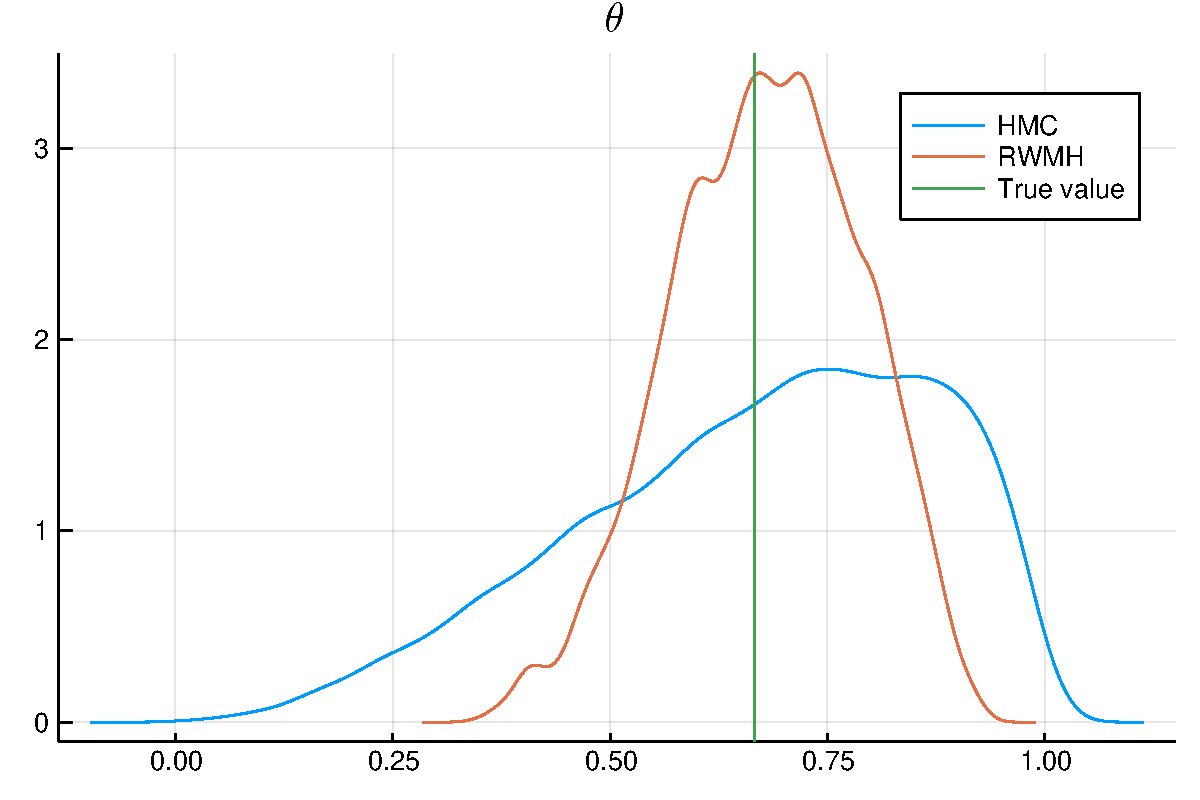
\includegraphics[width=\linewidth]{figures/dsge_and_julia_55_1.pdf}

\begin{lstlisting}
(*@\HLJLn{StatsPlots}@*)(*@\HLJLoB{.}@*)(*@\HLJLnf{density}@*)(*@\HLJLp{(}@*)(*@\HLJLn{pars{\_}hmc10k}@*)(*@\HLJLp{[}@*)(*@\HLJLoB{:}@*)(*@\HLJLp{,}@*)(*@\HLJLni{4}@*)(*@\HLJLp{],}@*) (*@\HLJLn{label}@*) (*@\HLJLoB{=}@*) (*@\HLJLs{"{}HMC"{}}@*)(*@\HLJLp{)}@*)
(*@\HLJLn{StatsPlots}@*)(*@\HLJLoB{.}@*)(*@\HLJLnf{density!}@*)(*@\HLJLp{(}@*)(*@\HLJLn{pars{\_}convertidos10k}@*)(*@\HLJLp{[}@*)(*@\HLJLni{1}@*)(*@\HLJLoB{:}@*)(*@\HLJLni{10000}@*)(*@\HLJLp{,}@*)(*@\HLJLni{4}@*)(*@\HLJLp{],}@*) (*@\HLJLn{label}@*) (*@\HLJLoB{=}@*) (*@\HLJLs{"{}RWMH"{}}@*)(*@\HLJLp{)}@*)
(*@\HLJLnf{title!}@*)(*@\HLJLp{(}@*)(*@\HLJLso{L"{}{\textbackslash}sigma"{}}@*)(*@\HLJLp{)}@*)
(*@\HLJLnf{vline!}@*)(*@\HLJLp{([}@*)(*@\HLJLn{true{\_}pars}@*)(*@\HLJLp{[}@*)(*@\HLJLsc{:sig}@*)(*@\HLJLp{]],}@*) (*@\HLJLn{label}@*) (*@\HLJLoB{=}@*) (*@\HLJLs{"{}True}@*) (*@\HLJLs{value"{}}@*)(*@\HLJLp{)}@*)
\end{lstlisting}

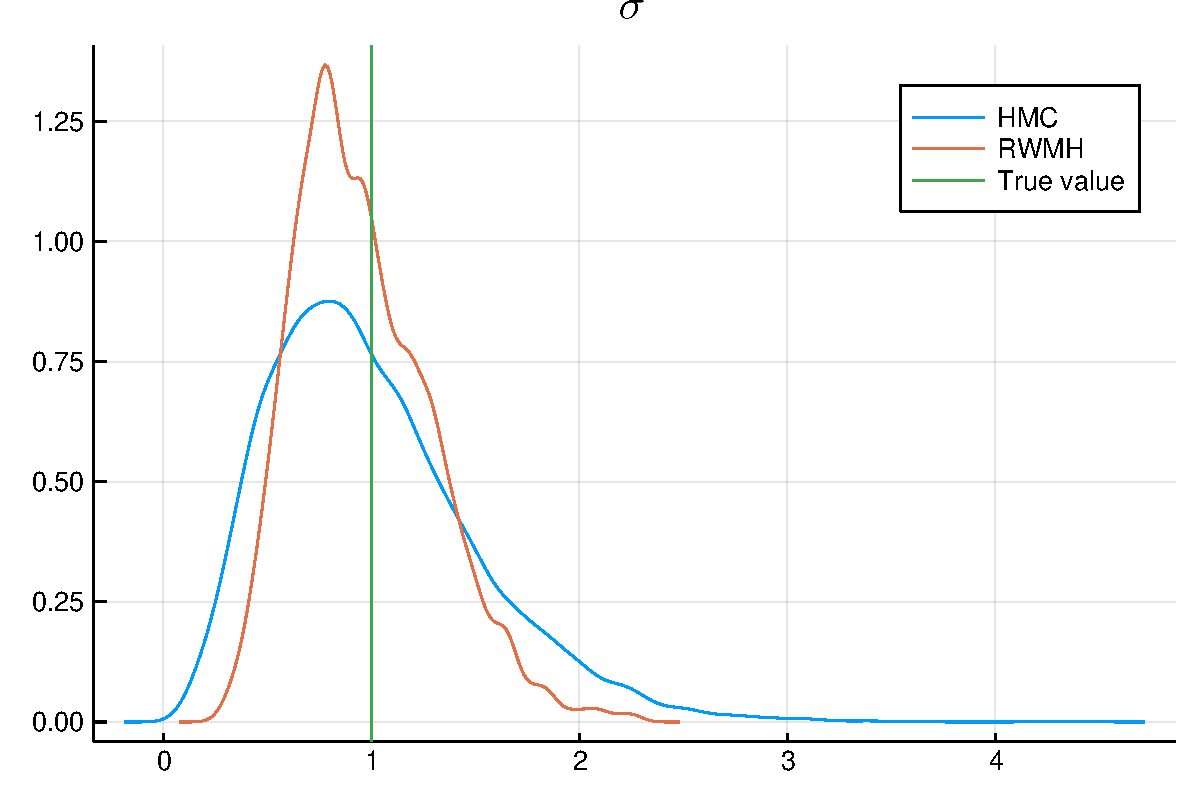
\includegraphics[width=\linewidth]{figures/dsge_and_julia_56_1.pdf}

\begin{lstlisting}
(*@\HLJLn{StatsPlots}@*)(*@\HLJLoB{.}@*)(*@\HLJLnf{density}@*)(*@\HLJLp{(}@*)(*@\HLJLn{pars{\_}hmc10k}@*)(*@\HLJLp{[}@*)(*@\HLJLoB{:}@*)(*@\HLJLp{,}@*)(*@\HLJLni{5}@*)(*@\HLJLp{],}@*) (*@\HLJLn{label}@*) (*@\HLJLoB{=}@*) (*@\HLJLs{"{}HMC"{}}@*)(*@\HLJLp{)}@*)
(*@\HLJLn{StatsPlots}@*)(*@\HLJLoB{.}@*)(*@\HLJLnf{density!}@*)(*@\HLJLp{(}@*)(*@\HLJLn{pars{\_}convertidos10k}@*)(*@\HLJLp{[}@*)(*@\HLJLni{1}@*)(*@\HLJLoB{:}@*)(*@\HLJLni{10000}@*)(*@\HLJLp{,}@*)(*@\HLJLni{5}@*)(*@\HLJLp{],}@*) (*@\HLJLn{label}@*) (*@\HLJLoB{=}@*) (*@\HLJLs{"{}RWMH"{}}@*)(*@\HLJLp{)}@*)
(*@\HLJLnf{title!}@*)(*@\HLJLp{(}@*)(*@\HLJLso{L"{}{\textbackslash}sigma{\textasciicircum}2"{}}@*)(*@\HLJLp{)}@*)
(*@\HLJLnf{vline!}@*)(*@\HLJLp{([}@*)(*@\HLJLn{true{\_}pars}@*)(*@\HLJLp{[}@*)(*@\HLJLsc{:s2}@*)(*@\HLJLp{]],}@*) (*@\HLJLn{label}@*) (*@\HLJLoB{=}@*) (*@\HLJLs{"{}True}@*) (*@\HLJLs{value"{}}@*)(*@\HLJLp{)}@*)
\end{lstlisting}

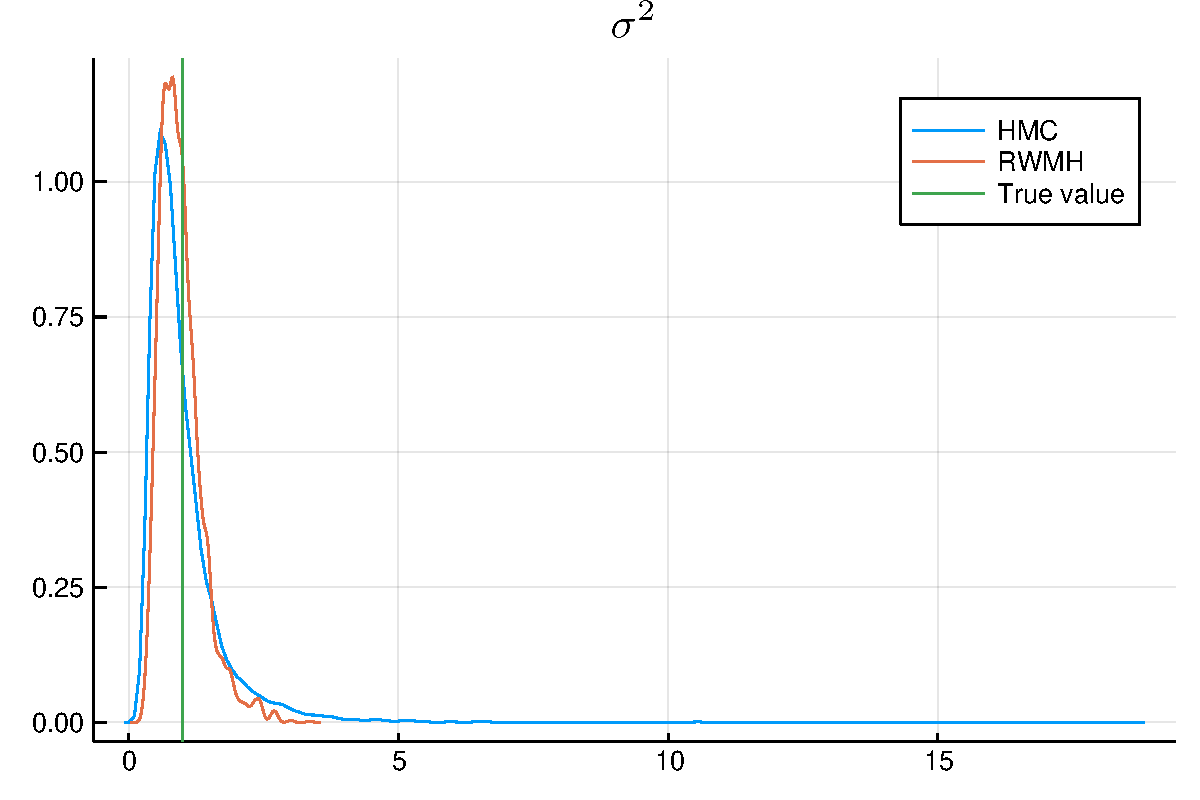
\includegraphics[width=\linewidth]{figures/dsge_and_julia_57_1.pdf}

\begin{lstlisting}
(*@\HLJLn{StatsPlots}@*)(*@\HLJLoB{.}@*)(*@\HLJLnf{density}@*)(*@\HLJLp{(}@*)(*@\HLJLn{pars{\_}hmc10k}@*)(*@\HLJLp{[}@*)(*@\HLJLoB{:}@*)(*@\HLJLp{,}@*)(*@\HLJLni{6}@*)(*@\HLJLp{],}@*) (*@\HLJLn{label}@*) (*@\HLJLoB{=}@*) (*@\HLJLs{"{}HMC"{}}@*)(*@\HLJLp{)}@*)
(*@\HLJLn{StatsPlots}@*)(*@\HLJLoB{.}@*)(*@\HLJLnf{density!}@*)(*@\HLJLp{(}@*)(*@\HLJLn{pars{\_}convertidos10k}@*)(*@\HLJLp{[}@*)(*@\HLJLni{1}@*)(*@\HLJLoB{:}@*)(*@\HLJLni{10000}@*)(*@\HLJLp{,}@*)(*@\HLJLni{6}@*)(*@\HLJLp{],}@*) (*@\HLJLn{label}@*) (*@\HLJLoB{=}@*) (*@\HLJLs{"{}RWMH"{}}@*)(*@\HLJLp{)}@*)
(*@\HLJLnf{title!}@*)(*@\HLJLp{(}@*)(*@\HLJLso{L"{}{\textbackslash}phi"{}}@*)(*@\HLJLp{)}@*)
(*@\HLJLnf{vline!}@*)(*@\HLJLp{([}@*)(*@\HLJLn{true{\_}pars}@*)(*@\HLJLp{[}@*)(*@\HLJLsc{:phi}@*)(*@\HLJLp{]],}@*) (*@\HLJLn{label}@*) (*@\HLJLoB{=}@*) (*@\HLJLs{"{}True}@*) (*@\HLJLs{value"{}}@*)(*@\HLJLp{)}@*)
\end{lstlisting}

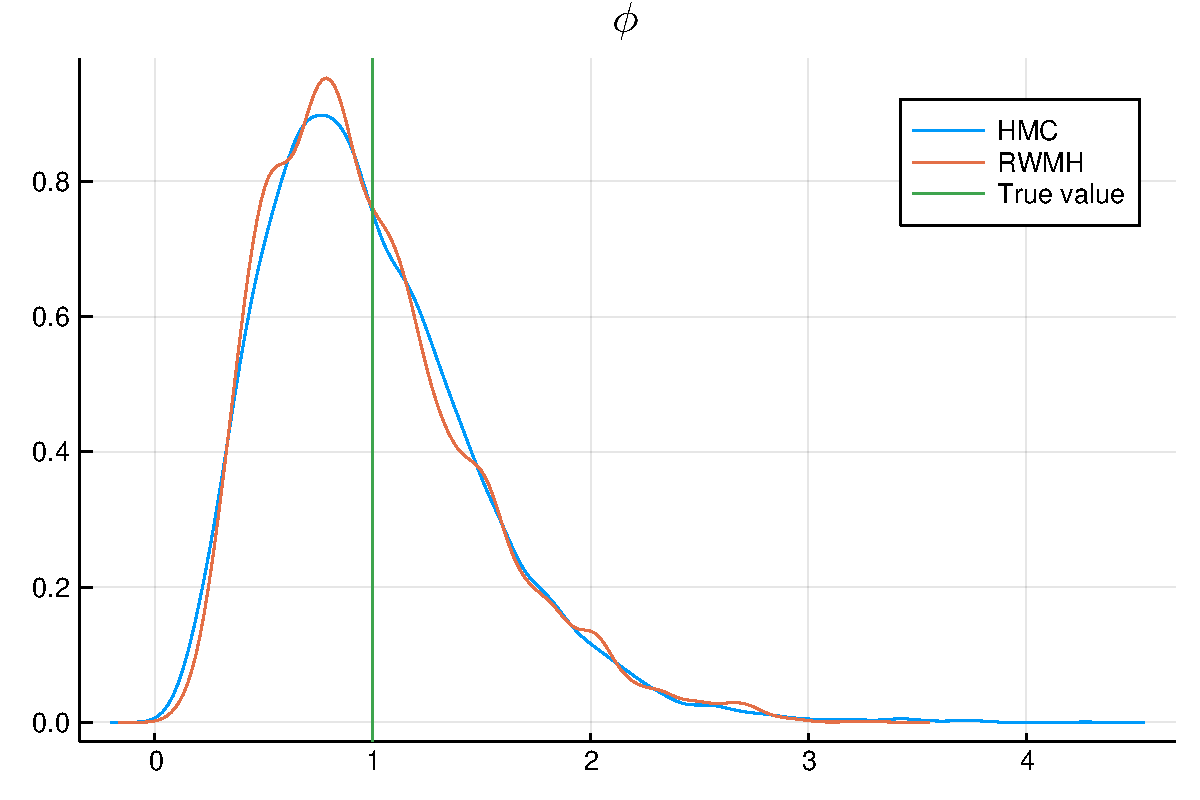
\includegraphics[width=\linewidth]{figures/dsge_and_julia_58_1.pdf}

\begin{lstlisting}
(*@\HLJLn{StatsPlots}@*)(*@\HLJLoB{.}@*)(*@\HLJLnf{density}@*)(*@\HLJLp{(}@*)(*@\HLJLn{pars{\_}hmc10k}@*)(*@\HLJLp{[}@*)(*@\HLJLoB{:}@*)(*@\HLJLp{,}@*)(*@\HLJLni{7}@*)(*@\HLJLp{],}@*) (*@\HLJLn{label}@*) (*@\HLJLoB{=}@*) (*@\HLJLs{"{}HMC"{}}@*)(*@\HLJLp{)}@*)
(*@\HLJLn{StatsPlots}@*)(*@\HLJLoB{.}@*)(*@\HLJLnf{density!}@*)(*@\HLJLp{(}@*)(*@\HLJLn{pars{\_}convertidos10k}@*)(*@\HLJLp{[}@*)(*@\HLJLni{1}@*)(*@\HLJLoB{:}@*)(*@\HLJLni{10000}@*)(*@\HLJLp{,}@*)(*@\HLJLni{7}@*)(*@\HLJLp{],}@*) (*@\HLJLn{label}@*) (*@\HLJLoB{=}@*) (*@\HLJLs{"{}RWMH"{}}@*)(*@\HLJLp{)}@*)
(*@\HLJLnf{title!}@*)(*@\HLJLp{(}@*)(*@\HLJLso{L"{}{\textbackslash}phi{\_}{\{}{\textbackslash}pi{\}}"{}}@*)(*@\HLJLp{)}@*)
(*@\HLJLnf{vline!}@*)(*@\HLJLp{([}@*)(*@\HLJLn{true{\_}pars}@*)(*@\HLJLp{[}@*)(*@\HLJLsc{:phi{\_}pi}@*)(*@\HLJLp{]],}@*) (*@\HLJLn{label}@*) (*@\HLJLoB{=}@*) (*@\HLJLs{"{}True}@*) (*@\HLJLs{value"{}}@*)(*@\HLJLp{)}@*)
\end{lstlisting}

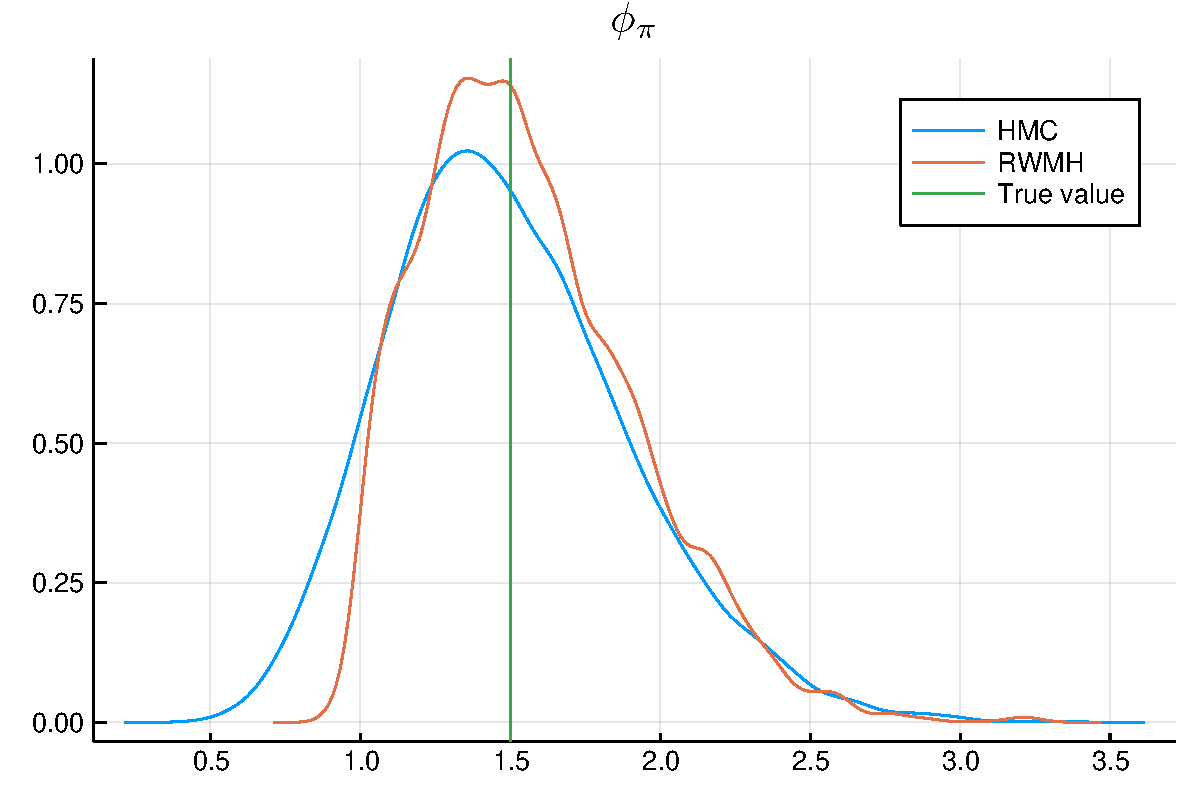
\includegraphics[width=\linewidth]{figures/dsge_and_julia_59_1.pdf}

\begin{lstlisting}
(*@\HLJLn{StatsPlots}@*)(*@\HLJLoB{.}@*)(*@\HLJLnf{density}@*)(*@\HLJLp{(}@*)(*@\HLJLn{pars{\_}hmc10k}@*)(*@\HLJLp{[}@*)(*@\HLJLoB{:}@*)(*@\HLJLp{,}@*)(*@\HLJLni{8}@*)(*@\HLJLp{],}@*) (*@\HLJLn{label}@*) (*@\HLJLoB{=}@*) (*@\HLJLs{"{}HMC"{}}@*)(*@\HLJLp{)}@*)
(*@\HLJLn{StatsPlots}@*)(*@\HLJLoB{.}@*)(*@\HLJLnf{density!}@*)(*@\HLJLp{(}@*)(*@\HLJLn{pars{\_}convertidos10k}@*)(*@\HLJLp{[}@*)(*@\HLJLni{1}@*)(*@\HLJLoB{:}@*)(*@\HLJLni{10000}@*)(*@\HLJLp{,}@*)(*@\HLJLni{8}@*)(*@\HLJLp{],}@*) (*@\HLJLn{label}@*) (*@\HLJLoB{=}@*) (*@\HLJLs{"{}RWMH"{}}@*)(*@\HLJLp{)}@*)
(*@\HLJLnf{title!}@*)(*@\HLJLp{(}@*)(*@\HLJLso{L"{}{\textbackslash}phi{\_}y"{}}@*)(*@\HLJLp{)}@*)
(*@\HLJLnf{vline!}@*)(*@\HLJLp{([}@*)(*@\HLJLn{true{\_}pars}@*)(*@\HLJLp{[}@*)(*@\HLJLsc{:phi{\_}y}@*)(*@\HLJLp{]],}@*) (*@\HLJLn{label}@*) (*@\HLJLoB{=}@*) (*@\HLJLs{"{}True}@*) (*@\HLJLs{value"{}}@*)(*@\HLJLp{)}@*)
\end{lstlisting}

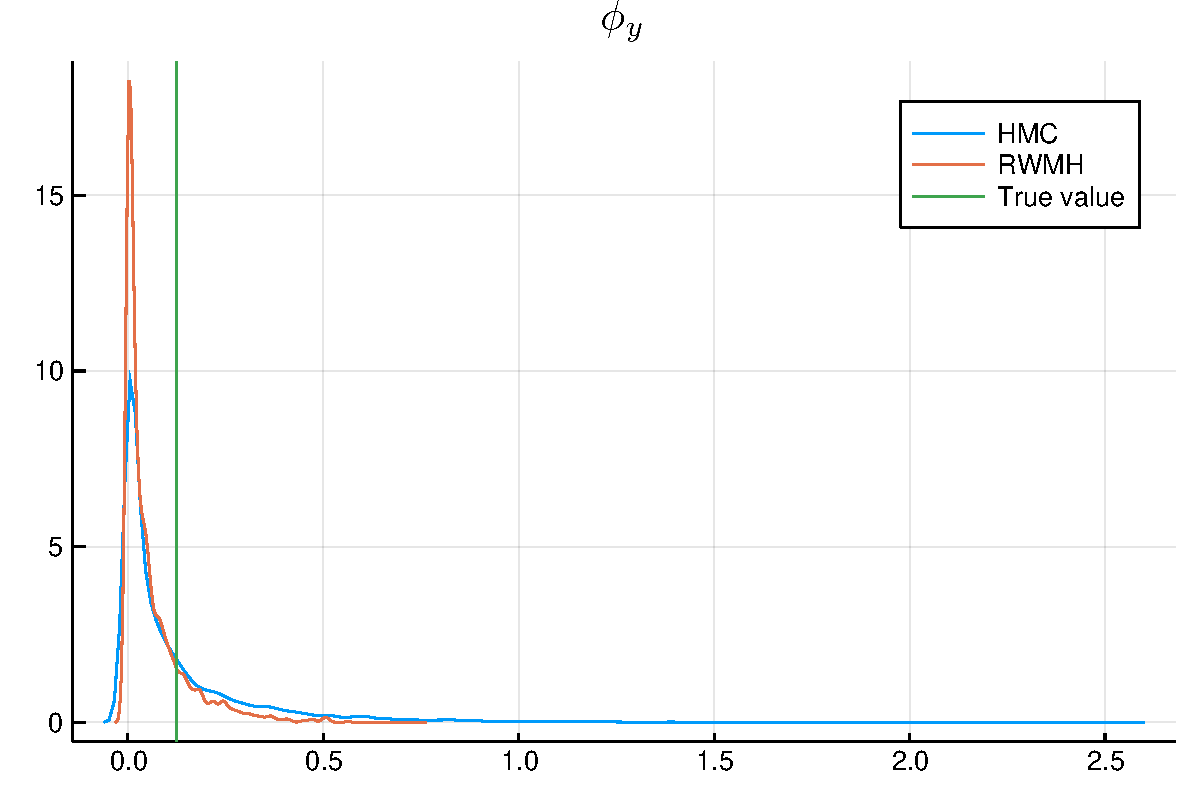
\includegraphics[width=\linewidth]{figures/dsge_and_julia_60_1.pdf}

\begin{lstlisting}
(*@\HLJLn{StatsPlots}@*)(*@\HLJLoB{.}@*)(*@\HLJLnf{density}@*)(*@\HLJLp{(}@*)(*@\HLJLn{pars{\_}hmc10k}@*)(*@\HLJLp{[}@*)(*@\HLJLoB{:}@*)(*@\HLJLp{,}@*)(*@\HLJLni{9}@*)(*@\HLJLp{],}@*) (*@\HLJLn{label}@*) (*@\HLJLoB{=}@*) (*@\HLJLs{"{}HMC"{}}@*)(*@\HLJLp{)}@*)
(*@\HLJLn{StatsPlots}@*)(*@\HLJLoB{.}@*)(*@\HLJLnf{density!}@*)(*@\HLJLp{(}@*)(*@\HLJLn{pars{\_}convertidos10k}@*)(*@\HLJLp{[}@*)(*@\HLJLni{1}@*)(*@\HLJLoB{:}@*)(*@\HLJLni{10000}@*)(*@\HLJLp{,}@*)(*@\HLJLni{9}@*)(*@\HLJLp{],}@*) (*@\HLJLn{label}@*) (*@\HLJLoB{=}@*) (*@\HLJLs{"{}RWMH"{}}@*)(*@\HLJLp{)}@*)
(*@\HLJLnf{title!}@*)(*@\HLJLp{(}@*)(*@\HLJLso{L"{}{\textbackslash}rho{\_}v"{}}@*)(*@\HLJLp{)}@*)
(*@\HLJLnf{vline!}@*)(*@\HLJLp{([}@*)(*@\HLJLn{true{\_}pars}@*)(*@\HLJLp{[}@*)(*@\HLJLsc{:rho{\_}v}@*)(*@\HLJLp{]],}@*) (*@\HLJLn{label}@*) (*@\HLJLoB{=}@*) (*@\HLJLs{"{}True}@*) (*@\HLJLs{value"{}}@*)(*@\HLJLp{)}@*)
\end{lstlisting}

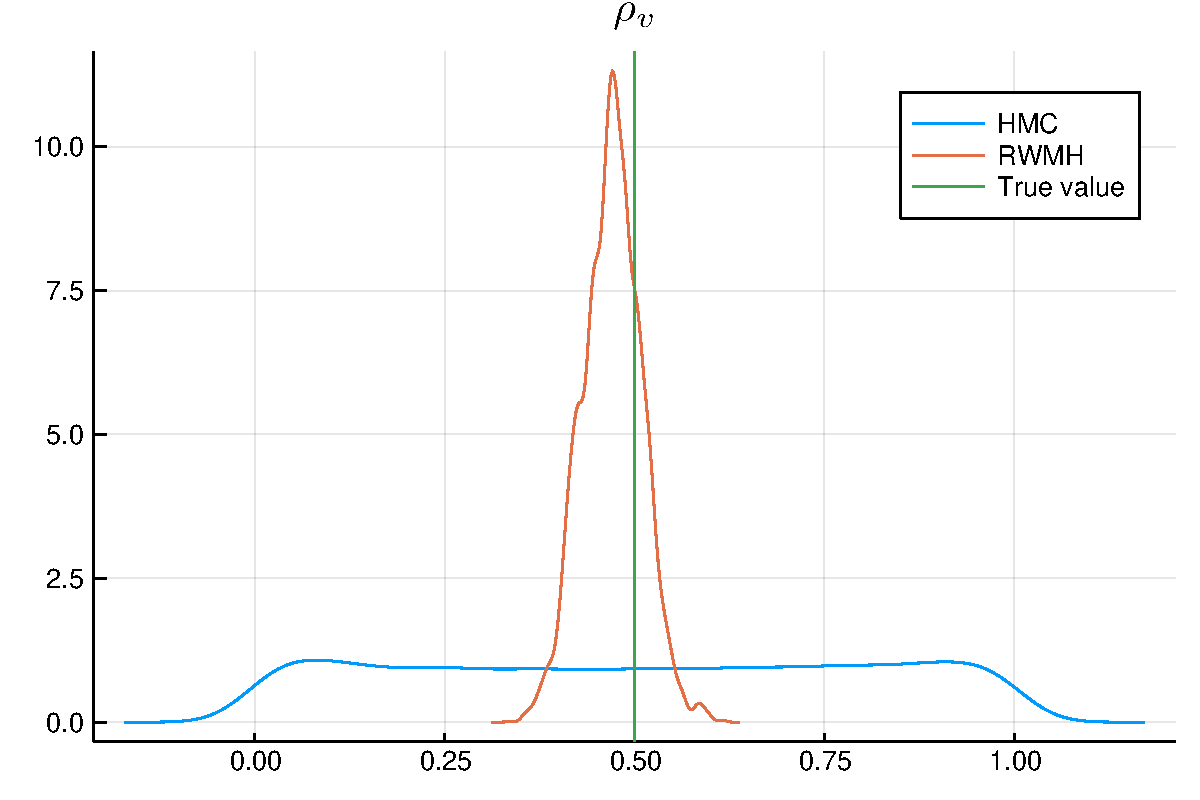
\includegraphics[width=\linewidth]{figures/dsge_and_julia_61_1.pdf}

Random Walk Metropolis Hasting distributions are never better behaved than the ones obtained from HMC - with the notable exception of the distribution of $\rho_v$However, the $\rho_v$ is not well behaved even with a hundred thousand iterations, so this is not due to the number of iterations.  

\bibliographystyle{authordate1}
\bibliography{DSGE}

\end{document}
